\documentclass[11pt]{article}

\usepackage[utf8]{inputenc}
\usepackage[T1]{fontenc}
\usepackage{amsmath,amssymb,amsthm}
\usepackage{graphicx}
\usepackage{booktabs}
\usepackage{longtable}
\usepackage[margin=2.5cm]{geometry}
\usepackage{xcolor}
\usepackage{hyperref}

\graphicspath{{figs/}}
\newcommand{\todo}[1]{{\color{red}\textbf{[TODO}\ifx\relax#1\relax\else: #1\fi\textbf{]}}}
\newcommand{\zenododoi}[1]{\href{https://doi.org/#1}{doi:#1}}
\newcommand{\repourl}{\url{https://github.com/jfbonder/universe25-abm}}

\title{An Agent-Based Model for the Social Collapse of Calhoun's Universe~25 Experiment}
\author{Julián Fernández Bonder\\[2pt]
{\small Departamento de Matemática, FCEN, Universidad de Buenos Aires, and}\\
{\small Instituto de Cálculo (UBA--CONICET), Buenos Aires, Argentina.}\\
{\small Email: \href{mailto:jfbonder@dm.uba.ar}{\texttt{jfbonder@dm.uba.ar}}}}
\date{Draft, \today}

\begin{document}

\maketitle

\begin{abstract}
We ask which \emph{local} interaction rules suffice to reproduce, qualitatively, the social collapse of Calhoun's
Universe~25, where a mouse colony with unlimited resources stopped reproducing and died out.
We study a lattice agent-based model in which each individual carries a social state, partly inherited, that
deteriorates under crowding, and we evaluate seventeen observed patterns run by run against null models.
Crowding and a long-lived demography alone already produce the envelope of the collapse: a peak well below
capacity, the end of natality, largely the social failure of late-born cohorts, and extinction.
Four local rules (a juvenile plasticity window, social learning, crowd aversion and refuges of limited capacity) add
coexisting crowded and isolated deteriorated classes, absent from most null models; the persistence of the isolated
class follows from the refuge design.
The full set of patterns holds in 99.5\% of the runs; with a small background mortality or spread initial ages it
falls to 55--63\%, only through a generic timing criterion.
The simulated dynamics is a boom of one or two generations rather than Calhoun's multi-generational sequence.
\end{abstract}

\section{Introduction}

Beginning in July 1968, John B.~Calhoun followed a population of house mice in a closed enclosure that he called
\emph{Universe~25} \cite{Calhoun1973}.
Food, water and nest space were in excess, predators and epidemic disease were excluded, and emigration was
impossible.
From four founding pairs the colony grew roughly exponentially.
It stopped growing at about 2200 animals, well below the 3840 the nest boxes could shelter.
The last young to survive weaning were born shortly after the peak, and the population then aged out without ever
recovering.
Along the way Calhoun described a breakdown of social behaviour:
\begin{itemize}
\item withdrawn males gathered in pools at the centre of the floor;
\item nursing females attacked and abandoned their young;
\item there appeared the unwounded, non-reproducing ``beautiful ones''.
\end{itemize}
Small groups moved to uncrowded enclosures during the decline did not reproduce, even with partners raised without
crowding (Marsden's work, reported in \cite{Calhoun1973}; see also \cite{Marsden1972}).
Calhoun read the collapse as a failure of social roles and of the maturation of complex behaviour, not of resources:
``density per se was not the major factor'' \cite{Calhoun1973}.
Section~\ref{sec:observations} lists the reported facts with page references.

The interpretation of the experiment has always been contested.
Its popular message, ``density causes pathology'', departed from Calhoun's own emphasis on social roles and design
\cite{RamsdenAdams2009,Ramsden2009,AdamsRamsden2024}.
Studies of human crowding found weak or no effects of density per se \cite{Galle1972,Freedman1975}.
For modelling, the decisive limitation is that Universe~25 was a single realization.
Calhoun himself called the study ``observation and reconstruction of a process; it was historical''
\cite{Calhoun1973}.
A model tuned to the published curve therefore risks fitting one sample path of a strongly stochastic process
\cite{GwizdallaDus2026}.

We ask instead:
\begin{quote}
Which \emph{local} interaction rules, with unlimited resources and no rule that depends on the total population,
generate robustly across stochastic realizations the part of Calhoun's sequence that runs from rapid growth to
extinction?
That part includes deceleration with social deterioration, cessation of reproduction near the peak, a decline
without recovery, and differentiated classes of deteriorated animals.
\end{quote}
The latency phase and the growth from four founding pairs are part of Calhoun's sequence, but we do not claim them:
our founder protocol reproduces them only partially (Section~\ref{sec:discussion}).
Our core model is a lattice model in which each mouse carries an age, a sex and a continuous social state $s_i\in[0,1]$.
The social state deteriorates under local crowding, scales conception and pup survival, and is partly inherited.
Movement is biased towards acquaintances.
We then add a few local rules, each with a neutral value that switches it off and recovers the core model, and each motivated by an
observation of the original report (Section~\ref{sec:model-rules}). Most have one principal parameter; the refuge
rule R7 has five and was designed after seeing the first candidate (Section~\ref{sec:limitations}):
\begin{itemize}
\item a juvenile window for social plasticity (R1);
\item social learning of competence (R2);
\item crowd aversion of deteriorated animals (AV);
\item refuges of limited capacity preferred by deteriorated animals (R7).
\end{itemize}
Rule names follow the simulation code; rules tested and discarded are listed in Section~\ref{sec:model-rules}.

Our contributions are the following. We separate throughout what is preregistered from what is post hoc, and what
the rules \emph{produce} from what they \emph{encode}.
\begin{enumerate}
\item We translate Calhoun's report, checked against the original, into seventeen falsifiable patterns, five
  refinements and four anti-patterns. Each has an operational criterion evaluated run by run, following
  pattern-oriented modelling \cite{Grimm2005}. We report the discriminating power of every essential criterion
  against four null models (no crowding damage; full inheritance without social learning; the long-lived demography
  without new rules; and the calibrated candidate without its four rules) and two partial ablations (no attraction,
  and the candidate without refuges) (Table~\ref{tab:res-null}). The preregistered forms of three criteria (O4, O10, O11) pass in null models; the primary evaluator,
  not preregistered, redefines them. O4 and O10 remain generic. O11 discriminates when the late cohorts are scored at six weeks
  of age, but not when they are scored at the end of the plasticity window. An additional
  desirable pattern (O10b, not preregistered) asks for a growth phase with socially competent adults.
\item We show that the core model without the rules, with a short life span (the short-lived control), is not
  Calhoun-like.
  About half of its colonies die in the first collapse, and the others oscillate with recovering natality.
  The mean-field analysis of that model traces the oscillations to spatial pockets of healthy individuals and to
  unconditional recovery.
  Removing the plasticity window from the calibrated model brings back recovery and recurrent natality at fast
  learning rates.
\item We separate what the rules add from what the demography, the crowding damage and the design of the rules
  already imply.
  \begin{itemize}
  \item \emph{The generic envelope.} A long-lived demography alone already drives every colony to extinction, so
    extinction is \emph{not} a result of the rules. With crowding damage and the calibrated attraction, the
    candidate without its four rules also has a low peak with free space (it passes the primary O4 in 200 of 200
    runs, with a peak at 0.45 of the damage-threshold capacity and 74\% of the cells empty), an end of natality and
    no rebound. Scored at the end of the plasticity window, its late-born cohorts also fail to acquire social
    competence (O11 in 0.755 of the runs, and 0.81 in the long-lived control), through accumulated crowding damage.
    These patterns verify that the model has a boom and its end; they are not evidence for the rules.
  \item \emph{Consistency checks of the design.} Some patterns follow from the rules by construction, and we report
    them as checks of the implementation, not as findings. Transplanted late-phase animals never found a colony
    (O12), because under the plasticity window R1 an adult cannot recover and conception is proportional to the
    social state of both partners, which is essentially zero in these animals. The isolated class is persistent
    (O13p) because the refuge capacity equals the isolation threshold. There are no social deaths (A4) and the decline
    is senescent (O8) because social mortality is switched off.
  \item \emph{What the rules add and the null models lack.} Two patterns: the coexistence of crowded and
    isolated deteriorated classes (O13), which needs crowd aversion or refuges and is a calibrated property of a
    nearly sessile regime; and the persistence of the isolated class (O13p), which is a design property. Both
    discriminate against three of the four null models, not against full inheritance without social learning. The
    failure of the late cohorts (O11) is not counted here. Scored at six weeks of age, as in the primary
    evaluator, it discriminates against all four null models, but that is partly definitional: pups are born
    below the deterioration threshold and are still inside the plasticity window. Scored at the end of the window,
    \textsf{C1} still passes (0.995), the dependence on the birth state disappears, and O11 discriminates against
    neither the long-lived nor the rule-free null model (0.81 and 0.755), whose late cohorts end even lower than
    those of \textsf{C1} (median $\bar s$ 0.07 and 0.06 against 0.13). The failure of the late cohorts is therefore mostly crowding damage.
\item \emph{What the dynamics is.} A boom of one or two generations, followed by a plateau without births or
    deaths and extinction by senescence. About 70\% of the births are to the founding animals, and the net
    reproductive number falls from 3.8 to 0.4 in a single generation (reference ensemble, 200 runs,
    Appendix~\ref{app:calib-generations}): pups are born below the deterioration threshold and learn from adults
    who have already deteriorated. The phases appear in Calhoun's order, but B and C are compressed, and we do not
    claim a cascade over many generations. The ratio of the deterioration time to the generation time, measured
    on animals past the plasticity window so that newborns do not dilute it, is $\Gamma=t_{\rm det}/T_{\rm gen}$
    $\approx1.1$ (1.2 on the founders), against about 3.5 in Universe~25 with a different operational definition; it is a heuristic
    comparison of time scales, not the cause of the shallow boom. With
    initial ages spread over 4--52 or 4--80 weeks the classes, the low peak and the failure of the late cohorts
    survive, but the timing of the end of natality relative to the peak (O5) does not (item~6).
  \end{itemize}
\item We identify which rules are needed, conditionally on the evaluation thresholds.
  With the class threshold of 10\%, isolation at $m\le2$, persistence of four weeks and the ensemble threshold of 0.8,
  the minimal set for the primary outcome is R1, R2 and R7 (candidate \textsf{C1}$'$, primary outcome in
  0.835 [0.78, 0.88] of 200 runs, borderline because the lower Wilson bound is below 0.8). With a class threshold of
  15\% it falls to 0.33, so minimality is not a property of the rules alone. Crowd aversion (AV) is a contributing
  rule: adding it (candidate \textsf{C1}) makes the primary outcome more reliable, through the generic criterion
  O5, and the decline senescent (O8); it \emph{reduces} the free space at the peak (16\% of the cells empty with
  AV, 52\% without). The contrast between \textsf{C1} and \textsf{C1}$'$ was not preregistered.
\item We test seven preregistered hypotheses (plan fixed on 1 October 2026, before the production runs; \texttt{docs/preregistered\_plan.md}).
  With the primary criteria the null hypothesis is rejected for six after Holm correction and the quantitative
  prediction holds for four (Q1, Q3, Q4, Q7); with the preregistered criteria the counts are five and four, and Q2 is
  not rejected. The only change that produces the rejection of Q2 is the post hoc choice of the end of natality in
  O5 (the 99th percentile of the births instead of the last birth), made after exploratory runs in which the
  alternative lowered the primary outcome of \textsf{C1} to about one half (Table~\ref{tab:deviations}). Two of the
  four predictions that hold are consistency checks, Q1 of R1 (above) and Q4 of the demography, and the
  preregistered contrast of Q3 is confounded by the demography. Q7 is confirmed only in the restricted sense stated
  in Section~\ref{sec:res-Q}. Removing crowd aversion lowers the primary outcome significantly with the primary criteria, but by much less than predicted; the predicted dependence on the length of the plasticity window (Q6)
  is not supported, because with the primary O11 the window has little or no effect on the boundary; and a
  predicted coexistence band (Q5) is refuted. Every deviation from the preregistered plan is listed in
  Table~\ref{tab:deviations}.
\item We report robustness in four senses. Against stochasticity it is high. Locally around \textsf{C1} it holds
  in most of the phase planes, with a nest period for pups (0.835 [0.78, 0.88], borderline) and with an
  asynchronous update (1.00). Globally it is limited and relative to the sampled box: the mean primary outcome over
  two 15-factor Latin hypercubes is 0.040 [0.026, 0.059], with 2.0\% of the points Calhoun-like, and the Sobol'
  indices are conditional on the factors fixed after screening. Demographically the primary outcome falls to 0.55
  with a background mortality of 0.003 per week and to 0.63 with initial ages spread over 4--80 weeks. Natality
  still ends with the population near its maximum, but the plateau starts earlier, so the last births fall more
  than half a peak time after its start and O5 becomes marginal (in 83 and 73 of the 90 and 74 runs that fail; the
  others fail it by the same timing clause). O5 is generic, and the patterns that the rules add (O13, O13p), as well as
  O11, pass in every one of these runs (Section~\ref{sec:limitations}).
\end{enumerate}
The model is documented with the ODD protocol \cite{Grimm2020} (Appendix~\ref{app:odd}), and the code is available in the repository \repourl.

\section{Related work}

\paragraph{Calhoun's experiments and their reception.}
Calhoun's programme of crowding experiments began with wild Norway rats in an outdoor enclosure.
There the population stabilized at about 150 adults, far below what adult survival would have allowed, because
of very high infant mortality \cite{Calhoun1962,Calhoun1963}.
It continued with laboratory ``universes'' for rats and mice, of which Universe~25 is the best known
\cite{Calhoun1973}.
His theoretical writings stress optimal group size and the saturation of social roles rather than physical density
\cite{Calhoun1971}.
The scientific and cultural history of these experiments, including the gap between Calhoun's interpretation and its
popular uptake, is treated in detail in \cite{RamsdenAdams2009,Ramsden2009,AdamsRamsden2024,Dugatkin2024}.
Earlier confined-population studies of house mice and other rodents had already reported that, with abundant food,
population growth stops through reduced litter survival and reproduction mediated by social interference
\cite{Southwick1955,Lidicker1965}.
This is the empirical basis of the coupling between social state and newborn survival in our model.

\paragraph{Models of Universe~25.}
Quantitative modelling of the experiment is very recent.
Gwizdałła and Duś \cite{GwizdallaDus2026} proposed an agent-based simulation with a daily time step and
empirically motivated life tables and litter-size distributions.
They calibrate the growth phase against the reported population and number of adults at day 315.
The decline is produced by deviation factors that are triggered when the total population exceeds critical values,
together with prescribed probabilities of litter abandonment and of becoming a ``beautiful one''.
They obtain the qualitative shape of the curve and approximate the timing of the peak.
They also emphasize the large dispersion across replicates and the lack of a methodological basis for the choice of
rules.
Mantzaris \cite{Mantzaris2025} attributes the collapse to the progressive loss of uncertainty about the social
hierarchy in a fully visible enclosure, implemented through a game-theoretic payoff matrix whose parameters change
across generations.
Roman \cite{Roman2025} fits maximum-entropy unimodal curves to the population time series without a mechanistic model.

Our approach differs from these in three respects:
\begin{enumerate}
\item all rules are local in space and use no global population thresholds;
\item the deterioration and its maternal transmission are dynamical variables rather than prescribed
  probabilities;
\item validation is based on multiple qualitative patterns evaluated as distributions over stochastic replicates,
  not on curve fitting.
\end{enumerate}

\paragraph{Social stress, maternal effects and population cycles.}
The idea that crowding acts through physiological stress on reproduction goes back to Christian's
adreno-pituitary hypothesis \cite{Christian1950}.
In the population-cycle literature, the transmission of individual quality from mother to offspring---the
\emph{maternal effect hypothesis}---produces delayed density dependence and cycles in simple two-variable models of
density and mean quality \cite{GinzburgTaneyhill1994,InchaustiGinzburg1998}.
Field evidence shows that maternal stress reduces reproduction and is carried over to the offspring
\cite{Sheriff2009}.
Our inherited social state is a spatially explicit, individual-based version of this mechanism.
Consistent with that theory, its mean-field limit has an oscillatory regime, which we show is not the one realized
in Universe~25.

\paragraph{Allee effects and stochastic extinction.}
Because reproduction requires that partners meet in the same cell, the model has a component Allee effect at low
density \cite{StephensSutherland1999,Courchamp2008}.
This has to be distinguished from social deterioration as an explanation for the absence of recovery.
Extinction is ultimately driven by demographic stochasticity acting on an absorbing state.
Mean times to extinction and their scaling with population size, quasi-stationary behaviour and extinction from the
troughs of cycles are reviewed in \cite{Ovaskainen2010}.
These provide the reference for our survival analysis of extinction times.

\paragraph{Methodology for agent-based models.}
We describe the model with the ODD protocol \cite{Grimm2020} and validate it in the spirit of pattern-oriented
modelling \cite{Grimm2005}.
For sensitivity analysis of stochastic agent-based models we follow the recommendations of ten Broeke et al.\
\cite{tenBroeke2016}: exploratory one-factor-at-a-time analysis to uncover mechanisms, followed by variance-based
global indices \cite{Saltelli2010}.
The number of replicates is chosen by the stability of output statistics \cite{Lorscheid2012}.
Although our aim is qualitative, the region of parameter space compatible with the reported patterns can be
characterized with approximate Bayesian computation using pattern-based summary statistics
\cite{Hartig2011,vanderVaart2015}.

\section{Observations to reproduce}
\label{sec:observations}

Because Universe~25 is a single realization, we do not fit the population curve.
Instead we extract from Calhoun's report \cite{Calhoun1973} a set of qualitative, falsifiable patterns and evaluate
each of them as a \emph{distribution over stochastic replicates}, in the spirit of pattern-oriented modelling
\cite{Grimm2005}.
Every pattern is translated into an operational criterion on simulated time series.
The criterion returns PASS, MARGINAL, FAIL or NOT APPLICABLE for each run.
For an ensemble we report the fraction of PASS runs with a 95\% Wilson interval.
An essential (E) pattern is considered reproduced if this fraction is at least $0.8$; a desirable (D) pattern if it is
at least $0.5$.
A criterion is informative only if it can fail. For every essential pattern we therefore also report its pass rate in
four null models run from the same initial condition: no crowding damage ($\gamma=0$), full inheritance without social
learning ($-$R2$^*$), the long-lived demography without new rules, and the calibrated candidate without its four
rules; and in two partial ablations, no attraction ($\alpha=0$) and the candidate without refuges (\textsf{C0})
(Table~\ref{tab:res-null}, Section~\ref{sec:res-null}). A pattern that passes in at least two of the four null models is
\emph{generic} and is not counted as evidence. The preregistered forms of O4, O10 and O11 pass in null
models, and the primary evaluator, which is not preregistered, redefines them (marked $^\S$ in
Table~\ref{tab:observations}): O10 is measured on adults, because pups are born with $s\le w\,s_f\le0.2$ and dilute
the mean in any growing colony; O11 does not pass when no animal is born in its window; and O4 also requires free
space at the peak. O4 and O10 remain generic. O11, scored at sexual
maturity (six weeks), discriminates against every null model, but in part because pups are born below its
threshold; scored at the end of the plasticity window it also passes in most runs of the long-lived and rule-free
null models (0.81 and 0.755; Section~\ref{sec:res-null}), so the failure of the late cohorts is mostly crowding damage. The free-space condition of O4, $f_0\ge0.10$, turns into a criterion what had been an informal
target of the calibration, used to discard candidates (Section~\ref{sec:circularity}). An additional desirable pattern,
O10b, asks for a growth phase with socially competent adults, as in Calhoun's phase B. These redefinitions were made
after seeing the data and are listed among the deviations from the preregistered plan (Table~\ref{tab:deviations}).
Patterns that follow from the rules by construction are marked $^\ddagger$ and reported as consistency checks.
One model step is one week.
Calhoun's dates are converted to weeks and enter only through dimensionless ratios: $t_{\rm pk}$ is the time of the
population peak, $N_{\rm pk}$ the peak size, and $t_{B0}$ the time at which surviving births cease. The table states
the criteria with these symbols; the primary evaluator replaces $t_{\rm pk}$ by the start of the plateau $t'_{\rm pk}$
(the first week with $N\ge0.98\,N_{\rm max}$) and, in O5, $t_{B0}$ by the week $t_{B99}$ at which 99\% of the births
have occurred (Section~\ref{sec:stats}, Table~\ref{tab:deviations}).
Table~\ref{tab:observations} lists the patterns, and Table~\ref{tab:calhoun-numbers} the numbers taken from the
original report.
Page numbers refer to \cite{Calhoun1973}.

{\small
\begin{longtable}{@{}p{0.06\textwidth}p{0.04\textwidth}p{0.47\textwidth}p{0.35\textwidth}@{}}
\caption{Qualitative patterns (O) and anti-patterns (A). E = essential, D = desirable, X = exploratory.
$^\dagger$O13p is not preregistered (defined after calibration) and enters the primary outcome O17p $=$ O17 $\wedge$
O13p (Section~\ref{sec:limitations}). O17p is strict: a not-applicable essential pattern counts as a failure (except
O1--O3 when $N_0>20$, which are excluded by design), and an evaluation error is never a pass. O17 alone counts
not-applicable patterns as passes, so we do not cite it. $^\ddagger$Consistency check of the design: the pattern follows from the rules
by construction (O12 from R1 and $p_{\rm conc}\propto s_fs_m$; O13p from R7 with $c_R=2$; O8 and A4 from $\mu_s=0$)
and is reported as a check, not as a finding (Section~\ref{sec:discussion}). $^\S$Not preregistered: the
preregistered form also passes in null models (Table~\ref{tab:res-null-v1}); in the primary form O4 and O10 are
still generic. Primary evaluator: $t_{\rm pk}\to t'_{\rm pk}$ in every criterion, $t_{B0}\to t_{B99}$ in O5, $f_0$
measured at $t'_{\rm pk}$, crowded class at $m>8$. $K_\gamma=m_c|G|$ is the population at
which every cell would sit at the damage threshold; it is not a physical capacity. Full operational definitions are
in the supplementary specification.}\label{tab:observations}\\
\toprule
ID & & Observation in Universe~25 (page in \cite{Calhoun1973}) & Operational criterion \\
\midrule
\endfirsthead
\toprule
ID & & Observation (cont.) & Criterion \\
\midrule
\endhead
\bottomrule
\endfoot
O1 & E & 104 days of ``considerable social turmoil'' before the first litters (p.~82) & founder scenario only: $t_{\rm lag}/t_{\rm pk}\in[0.10,0.35]$ (Calhoun $0.19$) \\
O2 & E & Exponential growth, doubling time ``about 55 days'' (p.~83) & $R^2\ge 0.90$ for $\log N$ in the growth window \\
O3 & E & Doubling time rises to ${\approx}145$ days from $N=620$ (pp.~83--84) & $r_B/r_C\ge 2$, phase C lasting $\ge 0.1\,t_{\rm pk}$ \\
O4 & E$^\S$ & Peak of 2200 versus shelter for 3840, food for 9500 and water for 6144; 20\% of nest boxes empty at the peak (p.~82) & $N_{\rm pk}/K_\gamma\le 0.8$ and empty fraction of cells at the peak $f_0\ge0.10$ \\
O5 & E & Growth ``abruptly ceased'' on day 560; last young surviving weaning born around day 600 (p.~85) & $N(t_{B0})/N_{\rm pk}\ge 0.7$ and $(t_{B0}-t_{\rm pk})/t_{\rm pk}\le 0.5$ \\
O6 & E & No recovery; the demise ``contradicts prior knowledge'' that remnant groups reinitiate growth (p.~85) & no rebound of $\ge 0.1N_{\rm pk}$, including slow regrowth still rising at censoring; birth-rate hysteresis $A_H\le 0.1$ \\
O7 & E & Total demise; last male projected dead on day 1780 (p.~85) & run: extinct by $T$; ensemble: $P_{\rm ext}(T)\ge 0.9$ (Kaplan--Meier) \\
O8 & D$^\ddagger$ & Decline through senescence; mean age of survivors 776 days (p.~85) & $(T_{\rm ext}-t_{\rm pk})/t_{\rm pk}\ge 1$ (Calhoun $\ge 1.84$ observed, $2.2$ projected) \\
O8b & D & Slow initial decline: $N=2056$ on day 736 (p.~83) & $N(1.31\,t_{\rm pk})/N_{\rm pk}\ge 0.8$ (Calhoun $0.93$) \\
O9 & D & 27 survivors (23 F, 4 M), all older than 987 days (p.~83) & no young in the remnant; female fraction $>0.5$ \\
O10 & E$^\S$ & ``death of societal organization by the end of Phase C'' (p.~85) & adult mean social state falls below 0.5 before the peak and stays below it at the peak: $t(\bar s_{\rm ad}<0.5)<t_{\rm pk}$, $\bar s_{\rm ad}(t_{\rm pk})<0.5$ \\
O10b & D$^\S$ & Phase B: 14 functional social groups during growth (days 104--315; pp.~83--84) & adults socially competent during growth: $t(\bar s_{\rm ad}<0.5)\ge 0.5\,t_{\rm pk}$ \\
O11 & E$^\S$ & From mid-phase C young ``prematurely rejected by their mothers''; complex behaviours fail to mature (p.~85) & social state at maturity decreasing across cohorts, and $<0.2$ for the cohorts born in the second half of natality; not applicable with fewer than 30 such animals (counts as failure in O17p) \\
O11b & D & Only 18\% of 148 late-phase-C females had ever conceived (p.~85) & fraction ever conceived $\le 0.3$ \\
O12 & E$^\ddagger$ & Small groups moved to uncrowded universes in mid-phase D failed to reproduce, even with partners raised without crowding (pp.~85--86) & transplant in silico: $P_T(D)\le 0.1$, $P_T(B)\ge 0.5$ \\
O13 & E & Withdrawn males pooled at the centre, wounded by other withdrawn males; ``beautiful ones'' unwounded, never courting or fighting (pp.~84--85, 88) & instantaneous coexistence of crowded ($m>m_c$) and isolated ($m\le2$) deteriorated classes, each $\ge 10\%$ of adults \\
O13p & E$^{\dagger\ddagger}$ & As O13, with a class that persists & isolated class persistent ($\ge4$ consecutive weeks) \\
O13b & D & Beautiful ones are a late, unsocialized cohort, ``the last half of the population born'' (p.~85) & isolated class born later than crowded class; $\ge 50\%$ born after $0.8\,t_{\rm pk}$ (post hoc variant: after the median birth time) \\
O14 & D & ``Behavioural sink'' on some hoppers (p.~81); births from 13 to 111 per brood group (pp.~83--84) & dispersion index $\ge 2$ at the peak; birth Gini above the $\alpha=0$ control \\
O15 & D & Conception declined, foetal resorption and pre-weaning loss increased; no surviving young after day 600 (p.~85) & infant mortality increasing, $\ge 0.9$ after $t_{B0}$ \\
O15b & D & Conceptions continued until about day 920 (p.~85) & $(t_{C0}-t_{B0})/t_{\rm pk}\ge 0.1$ (Calhoun $0.57$) \\
O16 & X & Nursing females aggressive towards own young; withdrawn males attack each other (pp.~84--85) & only with aggression rules \\
O17 & -- & Robustness criterion, not an observation. Motivated by the single realization: ``it was historical'' (p.~88) & run is Calhoun-like: all applicable E patterns pass, no anti-pattern; ensemble fraction $\ge 0.8$. Reported only through the strict primary outcome O17p \\
\midrule
A1 & & Logistic saturation at capacity & plateau within 10\% of $N_{\rm pk}$ for $\ge 100$ weeks \\
A2 & & Cycles with recovery of births & births resume to $\ge 10\%$ of maximum, or $\ge 2$ rebounds \\
A3 & & Demographic collapse before social collapse & per-capita fecundity halves only after $t_{\rm pk}$ \\
A4 & $^\ddagger$ & Adult death from deterioration as main cause & social share of deaths $\ge 0.5$ \\
\end{longtable}
}

\begin{table}[t]
\centering\small
\caption{Numbers reported in \cite{Calhoun1973} (days after colonization, DAC) and their conversion to weeks.
The model has no weaning period: ``last young surviving weaning'' is compared with the end of surviving births in the model
($t_{B0}$, pups that survive birth), which is an earlier event in the life of a pup.}
\label{tab:calhoun-numbers}
\begin{tabular}{@{}lrrl@{}}
\toprule
Event & DAC & weeks & page \\
\midrule
4 pairs of 48-day-old BALB/c mice introduced (9 July 1968) & 0 & 0 & 82 \\
First litters (end of phase A) & 104 & 14.9 & 82 \\
End of phase B: 620 weaned (150 adults in 14 groups, 470 juveniles) & 315 & 45 & 83--84 \\
Peak, $N=2200$ & 560 & 80 & 83, 85 \\
Last young surviving weaning & ${\sim}600$ & 85.7 & 83, 85 \\
$N=2056$ & 736 & 105 & 83 \\
Last conception & ${\sim}920$ & 131 & 85 \\
122 survivors (22 M, 100 F) & 1444 & 206 & 85 \\
27 survivors (23 F, 4 M), all older than 987 days & 1588 & 227 & 83 \\
Projected death of last male & 1780 & 254 & 85 \\
\bottomrule
\end{tabular}
\end{table}

\section{Model}
\label{sec:model}

The model is an individual-based, discrete-time stochastic process on a finite lattice. One time step
represents one week. Each individual carries four state variables: a position, an age, a sex and a
\emph{social state} $s_i\in[0,1]$, which summarises its capacity for normal social and reproductive
behaviour ($s=1$ fully competent, $s=0$ completely deteriorated). Individuals also keep a memory of
past contacts through a sparse affinity matrix. All rules are \emph{local}: no individual has access
to the population size or to any global statistic.

We first describe the \emph{core model} (Section~\ref{sec:model-baseline}): the lattice, the affinity matrix,
movement with attraction towards acquaintances, crowding damage to the social state, reproduction and senescent
mortality. Section~\ref{sec:model-rules} introduces four additional rules, R1, R2, AV and R7; each has a neutral
value that switches it off and leaves the core model unchanged. Section~\ref{sec:model-candidates} defines the four
calibrated candidates \textsf{C0}, \textsf{C1$'$}, \textsf{C1} and \textsf{C2} and the controls against which they are
compared, and Section~\ref{sec:model-groups} the dimensionless groups, the scales and the regimes we expect. The full
ODD description is in Appendix~\ref{app:odd}. Fig.~\ref{fig:model-schematic} summarises the ingredients and
Table~\ref{tab:params} lists all parameters.

\begin{figure*}[t]
  \centering
  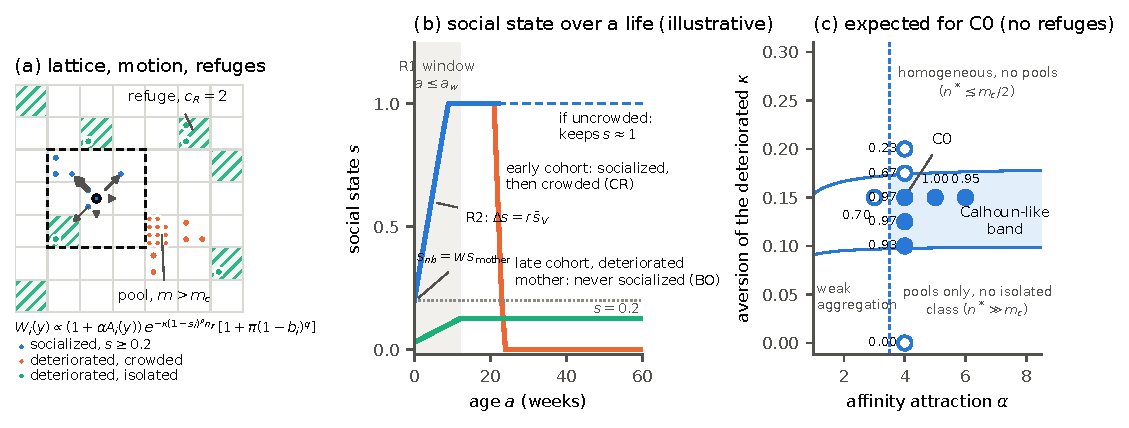
\includegraphics[width=\textwidth]{model_schematic.pdf}
  \caption{Schematic of the model.
  \textbf{(a)}~A focal agent (ringed) chooses a cell of its Moore neighbourhood (dashed) with the weight of
  Eq.~\eqref{eq:model-move}; arrow width is proportional to the weight. Deteriorated individuals gather in pools
  ($m>m_c$) or occupy refuges (hatched, capacity $c_R=2$).
  \textbf{(b)}~Illustrative trajectories of $s$ versus age, from
  Eqs.~\eqref{eq:model-social}--\eqref{eq:model-learning} with fixed environments (not a simulation). A pup
  starts at $w\,s_{\rm mother}$ and gains competence only inside the window $a\le a_w$ (R1), at a rate set by
  its neighbours (R2).
  \textbf{(c)}~Phase diagram expected for \textsf{C0} (no refuges). Crowded and isolated classes coexist in
  the shaded band, $5.5\lesssim n^*=1/\kappa-1/\alpha\lesssim10$ with $\alpha\gtrsim3.5$. Points are
  calibration ensembles of \textsf{C0} labelled with $f_{\rm O17}$; filled markers have $f\ge0.8$. With
  refuges the band disappears (Q5, refuted; Section~\ref{sec:results}).}
  \label{fig:model-schematic}
\end{figure*}

\subsection{Core model}
\label{sec:model-baseline}

\paragraph{Space and affinity.}
Individuals live on an $L\times L$ lattice $G$ ($L=30$, $|G|=900$) with hard boundaries. Any number of
individuals may share a cell; $m_i$ denotes the number of occupants of the cell of $i$, itself included.
Every pair of individuals at Chebyshev distance $\le1$ at the end of a week reinforces its affinity,
$F_{ij}\leftarrow(1-\eta)F_{ij}+\eta$. All other pairs decay, $F_{ij}\leftarrow(1-\delta)F_{ij}$, and pairs
with $F_{ij}<\varepsilon$ are forgotten ($\eta=0.2$, $\delta=0.01$, $\varepsilon=10^{-6}$). The affinity
memory is therefore long, $1/\delta=100$ weeks, and is built only by proximity.

\paragraph{Movement.}
Every week each individual moves to one of the nine cells $y$ of its Moore neighbourhood, its own cell
included, cells outside $G$ excluded. All individuals move simultaneously, using the positions at the
start of the week. The probability of choosing $y$ is proportional to
\begin{equation}
  W_i(y)=\bigl[1+\alpha A_i(y)\bigr]\;
         \underbrace{e^{-\kappa(1-s_i)^{p}n_y}}_{\text{aversion}}\;
         \underbrace{\bigl[1+\pi(1-b_i)^{q}\,\mathbf 1_{\mathcal R}(y)\bigr]\;
         \bigl[1-\mathbf 1_{\mathcal F}(y)\bigr]}_{\text{refuges}},
  \qquad A_i(y)=\sum_{j\in y}F_{ij},
  \label{eq:model-move}
\end{equation}
where $n_y$ is the number of \emph{other} individuals in $y$. A refuge cell is \emph{full} if it already holds
$n_y\ge c_R$ other individuals; $\mathcal R$ is the set of non-full refuges and $\mathcal F$ the set of full ones, so
that $\mathbf 1_{\mathcal R}(y)=1$ if $y$ is a non-full refuge and 0 otherwise, and $\mathbf 1_{\mathcal F}(y)=1$ if
$y$ is a full refuge and 0 otherwise.
In the core model only the first factor is present ($\kappa=0$, no refuges, $\mathcal R=\mathcal F=\emptyset$): the parameter
$\alpha\ge0$ sets the attraction towards acquaintances. The aversion and refuge factors are the
additional rules of Section~\ref{sec:model-rules}.

\paragraph{Social state.}
After moving, the social state is updated with the local occupancy,
\begin{equation}
  s_i\leftarrow\min\Bigl\{1,\max\bigl\{0,\;s_i+\varrho_i-\gamma\,(m_i-m_c)_+\bigr\}\Bigr\},
  \label{eq:model-social}
\end{equation}
where $\gamma(m_i-m_c)_+$ is the damage inflicted by each occupant in excess of the community size
$m_c=8$ ($\gamma=0.1$). In the core model the recovery term is a constant, $\varrho_i=r$ ($r=0.01$).
Deterioration is thus a purely local, density-triggered process, and its convexity in the local
occupancy makes it act as a switch (Section~\ref{sec:meanfield}).

\paragraph{Reproduction.}
Every reproductive female ($a_{\min}\le a\le a_{\rm rep}$) that shares her cell with at least one
reproductive male chooses one of them uniformly at random, and conceives with probability
\begin{equation}
  p_{\rm conc}=p_0\,s_f\,s_m,\qquad p_0=0.3 .
  \label{eq:model-repro}
\end{equation}
The litter size $\ell\in\{3,\dots,10\}$ is drawn from a fixed distribution with mean $\bar\ell=6.55$.
Each pup survives birth with probability $q_0\,s_f$ ($q_0=0.95$), so deteriorated mothers lose their
young. Newborns are placed in the mother's cell, have a 1:1 sex ratio, and inherit
$s_{\rm nb}=w\,s_f+(1-w)\,s_0$. The core model has full inheritance, $w=1$; this is its central
hypothesis, that the lack of maternal care propagates to the offspring.
There is no gestation delay, and a female may give birth every week.

\paragraph{Mortality.}
Every individual dies at the end of the week with probability
\begin{equation}
  p_{\rm death}(a,s)=\Bigl[1+e^{-k\,(a-a_{\max}[1-\mu_s(1-s)])}\Bigr]^{-1},\qquad k=0.15 .
  \label{eq:model-mort}
\end{equation}
The factor $\mu_s\ge0$ would advance the senescence of deteriorated individuals. Every model in this paper,
candidates and controls, has $\mu_s=0$, so adult death is purely senescent. Calhoun attributes the decline to senescence and describes the beautiful ones as
``physically healthy''~\cite{Calhoun1973}. Anti-pattern A4 and the senescent character of the decline (O8) therefore
hold by construction: they are consistency checks of the design, not results.
There is no mortality before senescence. The population therefore cannot decrease before the first senescent deaths:
once natality stops it sits on a plateau, and $t_{\rm pk}=\arg\max N$ falls on the last birth that precedes the first
death (exactly so in 69\% of the runs of \textsf{C1}). A constant background hazard $\mu_{\rm bg}$, independent of age
and $s$, is a reported variant; it acts at every age, pups included. With $\mu_{\rm bg}=0.003$ per week the plateau
shrinks from 51 to 17 weeks and the primary outcome falls to 0.55 [0.48, 0.62], through O5 alone, which becomes
MARGINAL rather than failing (83 MARGINAL and 7 FAIL among the 90 runs that do not pass). Natality still ends at the
population maximum, $N(t_{B99})\approx0.99\,N_{\rm pk}$. What moves is the start of the plateau: deaths now balance the
last births, so $t'_{\rm pk}$ comes earlier and the last 1\% of the births falls more than $0.5\,t'_{\rm pk}$ after
it. The coexisting classes (O13, O13p), the patterns that discriminate against the null models, pass in every
run, and so does O11, also with $\mu_{\rm bg}=0.008$, where O5 fails in 70 of 200 runs
(Section~\ref{sec:res-robustness}).

\paragraph{Longevity, order of events, initial condition.}
The candidates use $a_{\max}=120$ and $a_{\rm rep}=80$ weeks (the short-lived control below uses 60 and 50). These
values match the menopause at about 560 days and the frequent longevity of about 800 days in Universe~25~\cite{Calhoun1973},
and they allow a decline governed by ageing (O8). Each week the order is: movement, affinities, update of
$s$, reproduction, ageing, mortality. The initial condition is dispersed: $N_0=200+200$
individuals of age 4 weeks with $s=1$, at random positions. Non-synchronous variants draw the initial ages
uniformly over 4--52 or 4--80 weeks; the primary outcome is then 0.93 and 0.63, again through O5 alone and by the
same mechanism (with 4--80 weeks, 73 of the 74 runs that do not pass are MARGINAL, with
$N(t_{B99})\ge0.97\,N_{\rm pk}$; Section~\ref{sec:res-robustness}). The founder protocol is in Appendix~\ref{sec:calib-founders}.

\subsection{Minimal additional rules}
\label{sec:model-rules}

The core model reproduces the explosive growth and a density-triggered loss of social state, and with the long
life span nearly every colony dies too (Section~\ref{sec:results}). With a short life span ($a_{\max}=60$) it
does not reproduce three facts of Universe~25: the irreversibility of the collapse, the failure of the young born
during the crowded phase, and the coexistence of distinct classes of deteriorated animals. With the long-lived
demography used as a null model the first two are largely there: the colony does not rebound (O6 and O7 in 0.99,
1.00 without the rules at $\alpha=4$) and, scored at the end of the plasticity window, its late cohorts fail too
(O11 in 0.81, and in 0.755 without the rules; Section~\ref{sec:res-null}). Only the coexistence of classes is missing. R1 is still needed
once refuges exist, because refuges create pockets of low density in which, without an irreversible window,
deteriorated animals recover and breed again: without R1 natality resumes (O6 and O7 in 0.22, O17p 0.21), and
\textsf{C1} without R1 and R2 also fails them (0.35, with O13p in 0.05), whereas without R1 and without refuges
the collapse stays irreversible in most runs (O6 and O7 in 0.85 of 40 runs without R1 and R7; 1.00 without any rule; Appendix~\ref{app:res-ablations}). R1 is
what lets a persistent isolated class coexist with an irreversible collapse. A fourth fact, the low peak with free space, needs no new rule. With the
weak attraction $\alpha=1.4$ of the long-lived control (Section~\ref{sec:model-candidates}) the peak reaches 0.85 of $K_\gamma$, with 59\% of the cells
empty, so O4 fails only through the peak density. With the calibrated $\alpha=4$ and none of the rules below, the peak
stays at 0.45 with 74\% of the cells empty, and the primary O4 passes in every run (Table~\ref{tab:res-null}). The
low peak with free space is therefore a property of strong attraction with crowding damage, not of the rules. We add one rule for each of the three facts (R1, R2, and AV or R7 for the classes),
justified by an observation of the original report~\cite{Calhoun1973}. Each rule has one
principal parameter, but not only one: R2 also fixes the partial inheritance $(w,s_0)$, and R7 has five parameters
($f_R$, $c_R$, $\pi$, $q$ and the basis $b$) plus the choice of a hard capacity, and was designed after \textsf{C0} had
failed to produce a persistent isolated class (Section~\ref{sec:circularity}). Whether a rule is \emph{necessary} depends on
the others. In \textsf{C0} each of R1, R2 and AV is necessary (Section~\ref{sec:calib-ablations}). With
refuges (R7), AV is no longer necessary for the primary outcome; it then only shapes the spatial
organisation (Section~\ref{sec:results} and the paragraph on AV below). The minimal set for the primary
outcome is therefore R1 + R2 + R7, which defines the candidate \textsf{C1$'$} (Section~\ref{sec:model-candidates}).
This minimality is conditional on the evaluation thresholds (class threshold 0.10, isolation $m\le2$, persistence
$\ge4$ weeks, ensemble threshold 0.8; Section~\ref{sec:res-ablations}): \textsf{C1$'$} passes the primary outcome in
0.835 [0.78, 0.88] of the runs, with a lower bound below the threshold.

\paragraph{R1: critical window ($a_w$).}
Recovery is only possible for $a\le a_w=12$ weeks: $\varrho_i=0$ for older individuals, while crowding
damage acts at every age. An adult is therefore a ratchet, $\dot s_i\le0$.
\emph{Motivation.} Behaviours that failed to develop in youth were not acquired later. Animals moved from
the mid-third of phase~D to new universes at very low density, ``even placing them with adequate sex
partners \dots\ that had matured in uncrowded conditions'', showed no recovery of reproductive behaviour
(H.~Marsden's work reported in~\cite{Calhoun1973}; see also~\cite{Marsden1972}). R1 makes a deteriorated
cohort unable to recover by individual means. Since conception scales as $s_fs_m$, an adult with $s\simeq0$ can
neither recover nor reproduce, whatever its partner. The failure of phase-D transplants (O12) is therefore a
consistency check of R1, which was motivated by the same observation, and not an independent result.

\paragraph{R2: juvenile socialisation by neighbours ($\lambda$, with partial inheritance $w$).}
Recovery is \emph{learned} from the social environment:
\begin{equation}
  \varrho_i=r\bigl[(1-\lambda)+\lambda\,\bar s_{V(i)}\bigr],\qquad
  \bar s_{V(i)}=\frac{1}{|V(i)|}\sum_{j\in V(i)}s_j ,
  \label{eq:model-learning}
\end{equation}
where $V(i)$ contains the other individuals of the $3\times3$ block centred on $i$, and
$\bar s_{V(i)}=0$ for an isolated individual. We use $\lambda=1$, $r=0.1$, and partial inheritance
$s_{\rm nb}=w\,s_f$ with $w=0.2$, $s_0=0$. With R1, Eq.~\eqref{eq:model-learning} acts only on juveniles:
a pup starts with a fraction of its mother's competence and must acquire the rest from competent
neighbours before age $a_w$.
\emph{Motivation.} ``By midway in phase~C essentially all young were prematurely rejected by their
mothers. They started independent life without having developed adequate affective
bonds''~\cite{Calhoun1973}. Competence is transmitted socially. Once competent adults become scarce,
pups have nobody to learn from, and the state $s=0$ is absorbing for the population, not just for an
individual. In \textsf{C1} this transmission is shallow: it fails in a single step. Crowding deteriorates the
founders during their own adult life, within about one generation time. Their offspring, about 70\% of all births,
are born below the threshold and learn little, because their neighbours are mostly other pups and founders that are
already deteriorating. The net reproductive number falls from 3.8 daughters per founder female to 0.4 in the first
generation born, and 97\% of the births belong to the first two generations (Appendix~\ref{app:calib-generations}). R2 does not
produce a cascade over many generations; it makes the failure of the first generations born during the boom
irreversible for the colony.
With $w=0.2$ and $s_0=0$ every pup is born with $s_{\rm nb}\le0.2$, that is, at or below the threshold that the
patterns use for ``deteriorated''. Part of the failure of the crowded-born cohorts is therefore definitional: with
$s_0=0.25$ pups are born at $s_{\rm nb}\approx0.4$, and O11, which reads the state at the age of maturity
($a_{\min}=6$ weeks), passes in only 8\% of the runs, so that the primary outcome falls to 0.08
(Section~\ref{sec:res-robustness}). The essential part of R2 is social
learning, not inheritance. With refuges, $w=0$ and $r=0.15$ give the primary outcome in every run
(Section~\ref{sec:results}). We keep $w=0.2$ for continuity with the inheritance hypothesis of the core model.

\paragraph{AV: aversion of the deteriorated ($\kappa$).}
Deteriorated individuals avoid occupied cells through the factor $e^{-\kappa(1-s_i)^{p}n_y}$ of
Eq.~\eqref{eq:model-move}, with $\kappa=0.15$. The exponent $p=4$ is fixed, so that the aversion only
matters for $s\lesssim0.3$. The attraction $\alpha$ does \emph{not} depend on $s$. For a deteriorated
individual facing a cell with $n$ acquaintances ($A\simeq n$), the product $(1+\alpha n)e^{-\kappa n}$ is
maximal at
\begin{equation}
  n^*=\frac{1}{\kappa}-\frac{1}{\alpha},
  \label{eq:model-nstar}
\end{equation}
which is $6.4$ for the calibrated values, while cells of strangers are always avoided. Deteriorated
individuals therefore split between groups of a few times $m_c$, where crowding damage continues, and
almost empty cells.
\emph{Motivation.} Calhoun distinguishes withdrawn males, ``aggregated in large pools near the centre of
the floor'' and wounded ``as a result of attacks by other withdrawn males'', from the beautiful ones,
which ``never engaged in fighting'', carried ``no wound or scar tissue'' and ``never attempted to
enter'' social life~\cite{Calhoun1973}. In the model the damage term $\gamma(m-m_c)_+$ inside a pool is
damage inflicted by other deteriorated individuals, and isolated individuals receive none (objective
O13). Making $\alpha$ itself decrease with $s$ instead homogenises the population and raises the peak
(Section~\ref{sec:calib}).
\emph{Status.} AV is necessary in \textsf{C0}, where it alone generates the isolated class. With refuges it
is not necessary for the primary outcome: without AV it passes in 0.835 [0.78, 0.88] of the runs, against
0.995 [0.97, 1.00] (Section~\ref{sec:calib-ablations}). AV then controls the use of space and the decline. It
\emph{reduces} the free space: without it the deteriorated animals gather in a few pools and half of the lattice is
empty at the peak ($f_0=0.52$), with it $f_0=0.16$ (Universe~25: about 20\% of nest boxes). It also makes the
decline senescent (O8 0.625 against 0.21). Neither enters the preregistered outcome, which is why the minimal
candidate \textsf{C1$'$} omits AV. The low peak with free space itself needs no rule (see above).

\paragraph{R7: refuges with preference and hard capacity ($\pi$).}
A fixed random fraction $f_R=0.3$ of the cells are refuges of capacity $c_R=2$. Nobody may enter, or
stay in, a refuge that already holds $c_R$ other individuals. The capacity is \emph{hard}: after each
movement step residents keep their place, entrants are admitted in random order up to the capacity, and the
rejected ones return to their previous cell; admission is iterated until no refuge exceeds its capacity, and pups
that would be born in a full refuge are placed in a neighbouring cell that is not a refuge. A simpler
single-pass admission, which does not count returning animals and newborns and lets a refuge hold up to 11
individuals, is a reported variant; it leaves the primary outcome unchanged (0.995 with either rule;
Section~\ref{sec:res-robustness}).
Deteriorated individuals prefer refuges through the factor $1+\pi(1-b_i)^{q}$ of
Eq.~\eqref{eq:model-move}, where $b_i$ is the state that drives the retreat. In \textsf{C1}, $b_i=s_i$ with
$q=4$ and $\pi=100$. The total refuge capacity is $f_Rc_R|G|=540$ places, about 20\% of the
adult population at the peak.
\emph{Motivation.} The Universe~25 enclosure offered 256 nest boxes, each holding about 15 mice, and
would not have limited shelter below 3840 animals. At the peak about 20\% of the nest boxes were
usually unoccupied, because many mice chose to crowd together. Withdrawn females retreated to the high,
less preferred nests~\cite{Calhoun1973}.
\emph{Mapping.} We use a single mapping. Every cell is a resting site, the analogue of a nest box, and $m_c$
plays the role of the comfortable occupancy (15 per box in Universe~25, $m_c=8$ in the model), so that
$K_\gamma=m_c|G|$ is the analogue of the 3840 places and $f_0$ of the fraction of empty boxes. The refuges are the
analogue of the high, less preferred boxes (the upper one or two of the four levels of each tunnel, 25--50\% of the
boxes, against $f_R=0.3$). Their capacity $c_R=2$ is \emph{not} that of a nest box: it is the isolation threshold
$m\le2$ of O13, a design choice (Section~\ref{sec:circularity}). Neither $|G|$ nor $m_c$ was calibrated to
Universe~25, so densities are compared with Calhoun's only in sign (Appendix~\ref{app:calib-scales}).

Both the preference and the hard capacity are necessary with synchronous moves. Without a preference ($\pi=0$) the
refuges stay empty, because a deteriorated individual surrounded by acquaintances prefers an occupied neighbouring
cell. With a soft capacity, simultaneous moves produce stampedes (Appendix~\ref{sec:calib-classes}). The hard
capacity is a remedy for the collisions of the synchronous update: with a random sequential update a soft capacity
also produces a persistent isolated class (O17p 0.995, $\rho_{\rm pk}=0.43$ against 0.36;
Section~\ref{sec:res-robustness}).

\paragraph{Variant of R7 in \textsf{C2}: retreat driven by maternal socialisation.}
In \textsf{C2} the retreat is driven by the competence of the mother at birth, $b_i=h_i\equiv s_{f}(t_{\rm birth})$,
with $h_i=1$ for founders, $q=1$ and $\pi=1000$. Pups of deteriorated mothers retreat, and
socialised adults that later deteriorate do not, so they end up crowded.
\emph{Motivation.} The beautiful ones belonged to ``the last half of the population born''; they were
young animals that never entered social life, not adults that withdrew~\cite{Calhoun1973}.
Basing the retreat on juvenile competence (the value of $s$ at age $a_w$) fails. Under R2 almost every
cohort born after the first ends the window with $s<0.1$, so there is no gradient between cohorts.

\paragraph{Rules tested and rejected.}
Several rules were unnecessary or destroyed some pattern, and are not part of any candidate:
\begin{itemize}
  \item long-range jumps;
  \item an attraction that decreases with $s$;
  \item territoriality and defeat of males;
  \item social mortality;
  \item bonds restricted to competent pairs;
  \item movement sub-steps.
\end{itemize}
Mating in the Moore neighbourhood (\texttt{mate\_radius}${}=1$) only matters for the founder protocol.

\subsection{Calibrated candidates}
\label{sec:model-candidates}

We consider four candidates:
\begin{description}
  \item[\textsf{C0}] core model + longevity + R1 + R2 + AV. This is the minimal model that satisfies the essential
    patterns evaluable with $N_0=400$ when O13 is read instantaneously (O17 in 0.92 of the runs).
  \item[\textsf{C1$'$}] core model + longevity + R1 + R2 + R7 ($b=s$), without AV. This is the minimal set
    of rules for the preregistered primary outcome O17p (all essential patterns and a \emph{persistent}
    isolated class). See Section~\ref{sec:calib-ablations}.
  \item[\textsf{C1}] \textsf{C1$'$} + AV, equivalently \textsf{C0} + R7. AV adds the spatial organisation: it spreads
    the deteriorated animals over the lattice (the empty fraction at the peak falls from 0.52 to 0.16) and makes the
    decline senescent. \textsf{C1} is the reference of the production design.
  \item[\textsf{C2}] \textsf{C0} + R7 with the retreat driven by maternal socialisation ($b=h$). It makes the isolated
    class a later-born cohort.
\end{description}
The presets are \texttt{calhoun\_C0}, \texttt{calhoun\_C1p}, \texttt{calhoun\_C1} and \texttt{calhoun\_C2},
and Table~\ref{tab:params} lists their parameters.

\paragraph{Controls.}
A rule is switched off by its neutral value: $a_w=\infty$ for R1; $\lambda=0$ with full inheritance ($w=1$) and
individual recovery at the core rate $r=0.01$ for R2; $\kappa=0$ for AV; no refuge cells ($f_R=0$) for R7. Two
controls are the core model alone, with all four rules switched off, attraction $\alpha=1.4$ and the dispersed
initial condition:
\begin{description}
  \item[Short-lived control] a short life span, $a_{\max}=60$ and $a_{\rm rep}=50$ weeks;
  \item[Long-lived control] the life span of the candidates, $a_{\max}=120$ and $a_{\rm rep}=80$ weeks.
\end{description}
Table~\ref{tab:params} gives both in full. The null models of Section~\ref{sec:res-null} are run in a separate
ensemble and are defined relative to \textsf{C1}: no crowding damage ($\gamma=0$); $-$R2$^*$, \textsf{C1} with R2
switched off; the long-lived control; and ``no rules'', \textsf{C1} with all four rules switched off, which is the
long-lived control with the calibrated attraction $\alpha=4$. Two partial ablations of \textsf{C1} complete the
comparison: $\alpha=0$ (no attraction) and \textsf{C0} (no refuges).

\begin{table}[t]
  \centering
  \caption{Parameters of the short-lived (SL) and long-lived (LL) controls, which are the core model with the
  four rules switched off, and of the calibrated candidates \textsf{C0}, \textsf{C1$'$}, \textsf{C1} and \textsf{C2}.
  Time in weeks. A dash means that the rule is inactive. The code name is the field of \texttt{Params} in
  the \texttt{u25} package.}
  \label{tab:params}
  \small
  \resizebox{\textwidth}{!}{%
  \begin{tabular}{@{}lllcccccc@{}}
    \toprule
    Symbol & Meaning & Code name & SL & LL & \textsf{C0} & \textsf{C1$'$} & \textsf{C1} & \textsf{C2} \\
    \midrule
    \multicolumn{9}{@{}l}{\emph{Space, motion and affinity}}\\
    $L$ & lattice side (hard walls) & \texttt{grid\_size} & 30 & 30 & 30 & 30 & 30 & 30 \\
    $\alpha$ & attraction to acquaintances & \texttt{alpha} & 1.4 & 1.4 & 4.0 & 4.0 & 4.0 & 4.0 \\
    $\eta,\ \delta$ & affinity reinforcement, decay & \texttt{eta}, \texttt{delta} & 0.2, 0.01 & 0.2, 0.01 & 0.2, 0.01 & 0.2, 0.01 & 0.2, 0.01 & 0.2, 0.01 \\
    $\kappa,\ p$ & aversion of the deteriorated & \texttt{crowd\_aversion}, \texttt{\_power} & -- & -- & 0.15, 4 & -- & 0.15, 4 & 0.15, 4 \\
    \midrule
    \multicolumn{9}{@{}l}{\emph{Social state}}\\
    $m_c$ & community size & \texttt{m\_c} & 8 & 8 & 8 & 8 & 8 & 8 \\
    $\gamma$ & damage per excess occupant & \texttt{gamma} & 0.1 & 0.1 & 0.1 & 0.1 & 0.1 & 0.1 \\
    $r$ & recovery / learning rate & \texttt{rec} & 0.01 & 0.01 & 0.1 & 0.1 & 0.1 & 0.1 \\
    $a_w$ & R1 critical window & \texttt{plast\_age\_max} & $\infty$ & $\infty$ & 12 & 12 & 12 & 12 \\
    $\lambda$ & R2 weight of neighbours & \texttt{social\_rec\_lambda} & 0 & 0 & 1 & 1 & 1 & 1 \\
    $w,\ s_0$ & inheritance $s_{\rm nb}=w s_f+(1-w)s_0$ & \texttt{inherit\_weight}, \texttt{s\_newborn\_base} & 1, -- & 1, -- & 0.2, 0 & 0.2, 0 & 0.2, 0 & 0.2, 0 \\
    \midrule
    \multicolumn{9}{@{}l}{\emph{Refuges}}\\
    $f_R,\ c_R$ & refuge fraction, capacity (hard) & \texttt{refuge\_frac}, \texttt{\_capacity} & -- & -- & -- & 0.3, 2 & 0.3, 2 & 0.3, 2 \\
    $\pi,\ q$ & refuge preference & \texttt{refuge\_pref}, \texttt{\_power} & -- & -- & -- & 100, 4 & 100, 4 & 1000, 1 \\
    $b_i$ & state driving the retreat & \texttt{refuge\_pref\_basis} & -- & -- & -- & $s_i$ & $s_i$ & $h_i$ (mother) \\
    \midrule
    \multicolumn{9}{@{}l}{\emph{Demography}}\\
    $N_0$ & initial individuals (age 4, $s=1$) & \texttt{n\_males}+\texttt{n\_females} & 400 & 400 & 400 & 400 & 400 & 400 \\
    $p_0$ & conception probability & \texttt{p0} & 0.3 & 0.3 & 0.3 & 0.3 & 0.3 & 0.3 \\
    $q_0,\ \bar\ell$ & neonatal survival, mean litter & \texttt{neonatal\_survival} & 0.95, 6.55 & 0.95, 6.55 & 0.95, 6.55 & 0.95, 6.55 & 0.95, 6.55 & 0.95, 6.55 \\
    $a_{\min},\ a_{\rm rep}$ & reproductive ages & \texttt{repro\_age\_min}, \texttt{\_max} & 6, 50 & 6, 80 & 6, 80 & 6, 80 & 6, 80 & 6, 80 \\
    $a_{\max},\ k$ & senescence age, steepness & \texttt{a\_max}, \texttt{k\_mort} & 60, 0.15 & 120, 0.15 & 120, 0.15 & 120, 0.15 & 120, 0.15 & 120, 0.15 \\
    $\mu_s$ & social advance of senescence & \texttt{social\_mortality\_factor} & 0 & 0 & 0 & 0 & 0 & 0 \\
    \bottomrule
  \end{tabular}}
\end{table}

\subsection{Dimensionless groups, scales and expected regimes}
\label{sec:model-groups}

The qualitative behaviour depends on a few combinations of parameters; the values quoted are for \textsf{C1}. The
scales of the model and their counterparts in Universe~25 are listed in Appendix~\ref{app:calib-scales}.

\begin{itemize}
  \item $\Pi_\gamma=\gamma/r=1$: crowding damage per excess neighbour relative to the weekly learning rate.
  \item $\Lambda=r\,a_w=1.2$: the largest competence a juvenile can learn inside the window. A socialised
    lineage sustains itself only if $w+\Lambda\langle\bar s_V\rangle\gtrsim1$. Fast growth lowers the
    competence of the neighbours $\langle\bar s_V\rangle$, because novices outnumber teachers (a
    \emph{learning dilution}). Without crowding the colony goes extinct below a boundary in $(w,\Lambda)$ and grows
    without bound at the calibrated values (Q7). When $a_w$ is varied as well, $r$ and $a_w$ do not act through
    their product alone: the extinction transition is located only to within the spacing of the grid, and the local
    weight of $a_w$ relative to $r$ is about one half between $a_w=6$ and 12 weeks and about one between 12 and 24
    (Section~\ref{sec:res-Q}). Crowding is the trigger and R2 the amplifier.
  \item $n^*/m_c\approx0.8$ (Eq.~\eqref{eq:model-nstar}): the preferred group size of a deteriorated individual
    relative to the damage threshold. Without refuges it decides between pools, isolation, or both; with
    refuges it only marks the onset of homogenisation, near $n^*\approx3$--$4$ (Q5).
  \item $\phi_R=f_Rc_R|G|/N_{\rm ad}(t_{\rm pk})\approx0.2$: refuge capacity per adult at the peak. It bounds the
    persistently isolated fraction, $\Phi_{\rm BO}^{\rm pers}\le\phi_R$. The bound holds at all 50 points of the
    refuge plane, so a class of $\ge10\%$ needs $f_Rc_R\gtrsim0.3$; in that plane a persistent class appears only for
    $f_Rc_R\ge0.4$ and a strong preference (Section~\ref{sec:res-robustness}).
  \item $n_0=N_0/|G|=0.44$ and the Damk\"ohler number $\mathrm{Da}=t_{\rm mix}/t_{\rm det}$. Here
    $t_{\rm mix}=L^2/(4D_{\rm eff})$ is the time an individual needs to move across the lattice, with $D_{\rm eff}$ the
    mean squared displacement over 16 weeks divided by $4\times16$, and $t_{\rm det}=t_{1/2}-t_{\rm on}$ is the time
    the animals past the critical window (age $\ge a_w$) need to lose half of their competence ($t_{1/2}$, the first
    week with their mean $s<0.5$) after crowding sets in ($t_{\rm on}$, the first week with 5\% of the individuals in
    cells with $m>m_c$). These animals no longer learn, and newborns do not enter their mean until they leave the
    window, so $t_{\rm det}$ measures deterioration and not the dilution by pups born with $s\le0.2$. In \textsf{C1}
    $D_{\rm eff}\approx0.13$ cells$^2$ per week (8 exploratory runs), $t_{\rm mix}\approx1.7\times10^3$ weeks and
    $t_{\rm det}\approx10$ weeks ($t_{\rm on}=6$, $t_{1/2}=16$; reference ensemble), so
    $\mathrm{Da}\approx1.7\times10^2$. Deterioration is correlated over
    $\xi=(4D_{\rm eff}t_{\rm det})^{1/2}\approx2$ cells, the size of the contact neighbourhood. In founder colonies the
    relevant transport is the colonisation front: the filling time $t_{\rm fill}\approx t_{\rm pk}\approx170$--215
    weeks against $t_{\rm det}\approx20$--30 gives $\mathrm{Da}_{\rm fill}\approx10$
    (Appendix~\ref{sec:calib-founders}). In Universe~25 mice crossed the enclosure daily and the social organisation
    took a whole phase~C, about 35 weeks, to die, so $\mathrm{Da}\lesssim4\times10^{-3}$. The spatial structure of the
    model therefore emerges among animals that are almost sessile on the time scale of deterioration, which is not
    Calhoun's regime. Colonies grow from local nuclei, so $\rho_{\rm pk}$ falls with $n_0$, from 0.40 at $N_0=400$ to
    0.03 for eight founders.
  \item $\Gamma=t_{\rm det}/T_{\rm gen}\approx1.1$: deterioration time relative to the generation time,
    $T_{\rm gen}\approx9$ weeks (the interval between the median birth weeks of the first and second generations);
    the interquartile range over runs is 1.0--1.29, and the founders, a closed cohort, give 1.2. The mean over all
    animals of age $\ge a_{\min}=6$ would give 0.8, but that mean is diluted by the first generation, which
    enters it with $s\le0.2$ while still inside the window: when it falls below 0.5, in week 13, the founders still
    have $\bar s=0.66$ and are 39\% of those adults. Deterioration therefore takes of the order of one generation.
    The value depends on how $T_{\rm gen}$ is defined: with overlapping cohorts the interval between median birth
    weeks is not a demographic generation time, and in the null models it drops to 5 weeks (4 in some runs), below
    the age of first reproduction, which inflates their $\Gamma$ (1.4--1.6). With the standard demographic
    definition, the mean age of the mothers at birth ($T_{\rm gen}=14.3$ weeks in \textsf{C1}), $\Gamma\approx0.7$
    in \textsf{C1} and 0.60--0.85 in the other arms where it was computed; $\Gamma$ is of order one under either
    definition (Appendix~\ref{app:calib-generations}).
    $\Gamma$ does not set the depth of the boom. With five times less crowding damage ($\gamma=0.02$) $\Gamma=1.6$
    (1.8 on the founders), and the boom is still one to two generations deep: the mean generation of the births is
    1.42 against 1.35, $R_{\rm net}$ of the first generation is 0.52, and O17p passes in 17 of 20 runs. Pups born
    at $s_{\rm nb}\approx0.4$ ($s_0=0.25$) deepen the boom more at about the same $\Gamma$ (1.3): the mean
    generation is 1.51 and $R_{\rm net}=0.62$ (20 runs per point;
    Appendix~\ref{app:calib-generations}). The depth is set in the first step, from the founders to their offspring:
    pups are born below the deterioration threshold, conception and pup survival scale with the parents' state, and
    pups learn from neighbourhoods made mostly of other pups and of founders that are already deteriorating. In
    Universe~25 the deterioration took the whole phase~C, about 35 weeks, with $T_{\rm gen}\approx10$ weeks, so
    $\Gamma\approx3.5$ (our estimate). With a different operational definition, that is an order-of-magnitude
    comparison, not a test.
  \item \emph{Extinction time.} Without mortality before senescence, $T_{\rm ext}=\max_i(b_i+\ell_i)\simeq
    t_{\rm last}+\ell_{\max}$: the time of the last birth plus the longest residual lifetime. In \textsf{C1}
    $\ell_{\max}\approx110$ weeks with an interquartile range of a few weeks, of the order of the inverse slope of the
    logistic hazard, $1/k\approx7$ weeks. The spread of $T_{\rm ext}$ is therefore that of $t_{\rm last}$, the
    extreme of a sparse tail of births whose rate decays over $\tau_B=(t_{B99}-t_{B90})/\ln10\approx7$ weeks
    ($t_{Bq}$ is the week by which a fraction $q$ of all births has occurred). At fixed density the median of
    $T_{\rm ext}$ grows with the logarithm of the system size, from 162 weeks at $L=15$ to 184 at $L=60$, and its
    interquartile range over the median is 0.15 for $L\le20$ and about 0.08 for $L\ge30$
    (Appendix~\ref{app:calib-evs}). A small dispersion of $T_{\rm ext}$ is a property of how abruptly natality stops
    and of the size of the system, not a signature of the rules. In the same way
    $(T_{\rm ext}-t_{\rm pk})/t_{\rm pk}\approx2.1$ (Universe~25: $\ge1.84$) depends on where $t_{\rm pk}$ falls on the
    plateau: it is 4.0 if the peak time is the start of the plateau, $t'_{\rm pk}$, and the plateau itself shrinks
    from 51 to 17 weeks with a background mortality of 0.003 per week. Similarly $t_{\rm pk}/a_{\max}\approx0.45$
    (0.28 with $t'_{\rm pk}$), against 0.7 in Universe~25.
\end{itemize}

\paragraph{Expected regimes and their test.}
Before the production sweeps, the mean field (Section~\ref{sec:meanfield}) and the calibration suggested four
regimes. The production planes test them (Section~\ref{sec:results}). The planes report the fraction of runs that
pass a composite classifier (O17p). That fraction is not an order parameter, and its boundaries mix the mechanism
with the thresholds of the definitions. We therefore also report continuous order parameters: $\rho_{\rm pk}$, the
empty fraction $f_0$, the class order parameter $\Psi=\min(\Phi_{\rm BO}^{\rm pers},\Phi_{\rm CR})$ (O13p is
$\Psi\ge0.1$), the net reproductive number of the first generation and $\tau_B$ (Section~\ref{sec:res-robustness}; the widths of the
transitions could not be resolved with 20--30 runs per point).
\begin{enumerate}
  \item \emph{Recurrent growth} (A2), when recovery is individual and reversible. \emph{Confirmed}: without
    the window $P_{\rm ext}$ falls from 1 at $r=0.02$ to 0 for $r\ge0.2$.
  \item \emph{Unbounded growth} (A1), when crowding damage is weak or the population is homogenised.
    \emph{Confirmed} for $\gamma=0$.
  \item \emph{A single collapse without recovery}, the Calhoun-like regime. Extinction alone does not
    identify it, since the long-lived demography without new rules also goes extinct. What identifies it is
    the structure of the collapse, which requires R1 and R2. In \textsf{C0} the classes are set by
    $(\alpha,\kappa)$, inside the band of Fig.~\ref{fig:model-schematic}(c). With refuges the band
    disappears (Q5, refuted). No recovery appears in larger systems either: at fixed density, A2 is cleared in all
    150 exploratory runs with $L$ from 20 to 84 (30 per size, with the single-pass refuge admission), up to about
    21\,000 animals (Appendix~\ref{app:calib-evs}).
  \item \emph{Trivial early collapse}: founders in one cell, where local nuclei deteriorate before the colony
    spreads ($\mathrm{Da}_{\rm fill}\approx10$), or very strong aggregation.
\end{enumerate}
Persistence of the isolated class is a separate axis: it requires $\phi_R\gtrsim0.1$ and $\pi\gtrsim100$, and
its cohort structure depends on the basis $b$ of the retreat.

\section{Calibration of the candidates}
\label{sec:calib}

The rules of Section~\ref{sec:model} were not fitted to a population curve. They were selected, and their
parameters set, by maximising the number of qualitative patterns of Table~\ref{tab:observations} reproduced
across stochastic replicates, with the smallest set of rules. This section summarises that process. The
development ensembles, the local sensitivity analysis, the diagnosis of the deteriorated classes and the
founder protocol are in Appendix~\ref{app:calib}.

\paragraph{Calibration is not validation.}
\label{sec:circularity}
The rules and parameters were chosen with the same evaluator and the same patterns that are later reported
as reproduced. The production ensembles are statistically independent, but no pattern was held out.
Several modelling choices also mirror the operational definitions of the patterns:
\begin{itemize}
  \item the refuge capacity $c_R=2$ equals the isolation threshold $m\le2$ of O13;
  \item the persistence requirement of O13 was adopted after \textsf{C0} had been found to produce only
    transient isolation, and the refuges were then designed to satisfy it;
  \item $m_c$ is both the damage threshold and the threshold that defines the crowded class;
  \item the fraction of empty cells at the peak was used informally to discard candidates that left most of the
    lattice empty, and it is part of a criterion of the primary evaluator: the primary O4 requires $f_0\ge0.10$,
    so O4 tests a quantity that was an informal target of the calibration.
\end{itemize}
Reproducing O13 with refuges therefore shows that a persistent isolated class is \emph{possible} under local
rules; it is not a prediction. Several further patterns hold by construction and are consistency checks of the
design, not results:
\begin{itemize}
  \item the failure of phase-D transplants (O12, Q1): under R1 an adult cannot recover, and conception scales as
    $s_fs_m$, so animals with $s\simeq0$ cannot found a colony whatever their partners;
  \item the persistence of the isolated class (O13p), through $c_R=2$;
  \item the absence of social mortality (A4) and the senescent decline (O8), through $\mu_s=0$;
  \item the coincidence of the end of natality with the peak (O5) when the peak time is $\arg\max N$, because without
    mortality before senescence $t_{\rm pk}$ falls on the last birth before the first death
    (Section~\ref{sec:model-baseline}); measured from the start of the plateau, as in the primary evaluator, O5 is not
    automatic but generic: it passes in four of the null models (Table~\ref{tab:res-null});
  \item the life-table law of phase~D (Q4), which follows from the demography.
\end{itemize}
The tests that do not depend on the calibration targets are the relative weight of window and learning rate (Q6),
the endogenous collapse without crowding (Q7), both with the restrictions of Section~\ref{sec:res-Q}, and the
comparison with null models, in which a pattern that also passes carries no evidence (Section~\ref{sec:results}).
Agreements of magnitudes normalised by $t_{\rm pk}$, such as $(T_{\rm ext}-t_{\rm pk})/t_{\rm pk}\approx2.1$
(Calhoun: 2.2 projected), are not tests: they depend on where $t_{\rm pk}$ falls on the plateau
(Section~\ref{sec:model-groups}).

\paragraph{Procedure.}
\label{sec:calib-procedure}
Each run is scored by the evaluator of Section~\ref{sec:observations}. MARGINAL counts as not passing, and
ensemble fractions carry 95\% Wilson intervals. The calibration proceeded in five stages, with independent
seeds and a horizon of $T=600$ weeks:
\begin{enumerate}
  \item screening of rule families (47 points $\times$ 10 replicates);
  \item ablations of the selected rules (10 points $\times$ 40);
  \item one-at-a-time sensitivity (17 points $\times$ 30);
  \item development ensembles of the candidates, with 60--120 replicates and transplants;
  \item tests of the founder protocol.
\end{enumerate}
It used about 45~min on four cores. The transplant protocol and the stages are detailed in
Appendix~\ref{app:calib-procedure}.

\subsection{The candidates}
\label{sec:calib-candidates}

Table~\ref{tab:calib-candidates} lists the essential patterns of the four candidates of Table~\ref{tab:params} in
the production ensembles, with the exact hard capacity and the primary evaluator (the start of the
plateau $t'_{\rm pk}$ as peak time, O5 measured with the end of effective natality $t_{B99}$, the primary O4, O10
and O11, and the crowded class $m>8$). With the dispersed initial condition ($N_0=400$ at random positions), every
applicable essential pattern passes in at least 80\% of the runs of every candidate:
\begin{itemize}
  \item a low peak with free space (O4);
  \item natality ending at high $N$ (O5);
  \item no rebound (O6);
  \item extinction (O7);
  \item deterioration of the adults before the peak (O10);
  \item failure of the crowded-born cohorts (O11);
  \item failure of phase-D transplants (O12);
  \item two deteriorated classes (O13).
\end{itemize}
Only the candidates with refuges make the isolated class persistent (O13p) and thus pass the primary outcome
O17p. O1--O3 apply only to founder colonies (Appendix~\ref{sec:calib-founders}). Not all of these patterns carry the
same weight. O12 is a consistency check of R1 (see above). Against the null models of Table~\ref{tab:res-null}
only O13 and O13p discriminate, against three of the four (not against full inheritance without social learning).
O11 discriminates against all four only when scored at six weeks: at the end of the plasticity window it also passes
in 0.81 of the long-lived runs and in 0.755 of the runs without rules, so the failure of the late cohorts is mostly
crowding damage. O4, O5, O6, O7 and O10 pass in at least two null models and are generic. In particular the low peak with free space (O4) also passes in \textsf{C1} without its four
rules ($\rho_{\rm pk}=0.45$, $f_0=0.74$): it comes from the attraction $\alpha=4$ with crowding damage, not from the
rules. The development ensembles of Appendix~\ref{app:calib-dev} agree qualitatively.

\begin{table}[t]
  \centering
  \caption{Essential patterns of the four candidates in the production ensembles ($n=200$ each; exact
  hard capacity; primary evaluator; \textsf{C0}, \textsf{C1}$'$ and \textsf{C1} from the reference ensemble, \textsf{C2}
  from its contrast ensemble; Section~\ref{sec:res-production}, where the controls are also given). Fractions of
  passing runs. The 95\% Wilson half-width is at most 0.07, and at most 0.02 for fractions of 0 or 1. O17 uses the
  instantaneous O13; O17p, the primary outcome, also requires a persistent isolated class (O13p). O12: founding
  transplants of phase-D animals (taken at $1.75\,t'_{\rm pk}$) over trials (60 per candidate); with $s\simeq0$ it is a
  consistency check of R1. $\rho_{\rm pk}=N_{\rm pk}/K_\gamma$, with $K_\gamma=m_c|G|$ the damage-threshold capacity
  (not a physical capacity; Universe~25: 2200/3840 $=0.57$), and $f_0$, the median fraction of empty cells at the
  peak (Universe~25: about 20\% of nest boxes); both are comparable with Calhoun's only in sign.}
  \label{tab:calib-candidates}
  \small
  \resizebox{\textwidth}{!}{%
  \begin{tabular}{@{}lccccccccccc@{}}
    \toprule
    Candidate & O4 & O5 & O6 & O7 & O10 & O11 & O12 & O13 & O17 & O17p [95\% CI] & $\rho_{\rm pk}$ / $f_0$ \\
    \midrule
    \textsf{C0} (R1, R2, AV) & 1.00 & 1.00 & 1.00 & 1.00 & 1.00 & 1.00 & 0/60 & 0.92 & 0.92 & 0.00 [0.00, 0.02] & 0.41 / 0.18 \\
    \textsf{C1}$'$ (R1, R2, R7) & 1.00 & 0.855 & 1.00 & 0.995 & 1.00 & 0.975 & 0/60 & 1.00 & 0.835 & 0.835 [0.78, 0.88] & 0.33 / 0.52 \\
    \textsf{C1} (R1, R2, AV, R7) & 1.00 & 0.995 & 1.00 & 1.00 & 1.00 & 1.00 & 0/60 & 1.00 & 0.995 & 0.995 [0.97, 1.00] & 0.36 / 0.16 \\
    \textsf{C2} (\textsf{C1}, maternal $b$) & 0.90 & 0.815 & 0.98 & 0.98 & 1.00 & 0.995 & 0/60 & 1.00 & 0.725 & 0.705 [0.64, 0.76] & 0.42 / 0.11 \\
    \bottomrule
  \end{tabular}}
\end{table}

\subsection{Necessity of the rules}
\label{sec:calib-ablations}

Whether a rule is necessary depends on the others. Single ablations are in Table~\ref{tab:calib-ablations}
for \textsf{C0} and in Section~\ref{sec:res-ablations} for \textsf{C1} and \textsf{C1}$'$.

\paragraph{Without refuges (\textsf{C0}).} R1, R2 and AV are each necessary:
\begin{itemize}
  \item without R2, O11 and O13 are never reproduced (O17 0/40). Viable pups come from the healthiest
    mothers and inherit their competence;
  \item without AV, deteriorated animals collapse into a few pools, 76\% of the lattice is empty and the
    isolated class disappears;
  \item without R1, adults recover when the colony thins, and O17 falls to 0.40.
\end{itemize}

\paragraph{With refuges.} R7 supplies the isolated class, and AV is no longer necessary for the primary
outcome. The rules necessary for O17p are R1, R2 and R7: the single ablations of \textsf{C1}$'$ give O17p of 0 in
every case (40 runs each). AV is not: \textsf{C1}$'$, which is \textsf{C1} without AV, passes O17p in
0.835 [0.78, 0.88], against 0.995 [0.97, 1.00] for \textsf{C1}. This necessity is conditional on the thresholds of
the classes and of the ensemble (Section~\ref{sec:res-ablations}). What AV controls is the use of space, and it
\emph{reduces} the free space rather than supplying it: without AV the deteriorated animals gather in a few pools
and half of the lattice is empty at the peak ($f_0=0.52$), with AV $f_0=0.16$ (Universe~25: about 20\% of nest
boxes). It also controls the senescent decline, with O8 at 0.21 against 0.625. Partial inheritance is not necessary either:
\textsf{C1} with $w=0$ and $r=0.15$ passes O17p in all 120 runs. The essential part of R2 is social learning.

\paragraph{Crowding is the trigger.} Without crowding damage ($\gamma=0$) no colony collapses, and the mean
adult social state stays near 0.6. With the calibrated socialisation, the failure of socialisation under R2 needs
crowding to start (Q7): crowding deteriorates the founders, the only competent teachers, within about one
generation time ($\Gamma\approx1.1$; Section~\ref{sec:model-groups} and Appendix~\ref{app:calib-generations}).

\subsection{What the calibration does not achieve}
\label{sec:calib-limits}

\begin{enumerate}
  \item \emph{Founder colonies (O1--O3).} No candidate reproduces latency, exponential growth and
    deceleration robustly from four pairs. The best point of the founder plane reproduces O1--O3 jointly with O17p
    in 0.43 [0.27, 0.61] of the runs, and only with $a_{\max}=200$, outside the preset
    (Appendix~\ref{sec:calib-founders}).
  \item \emph{Initial condition.} The low peak ($N_{\rm pk}/K_\gamma\approx0.4$) holds for the
    dispersed initial condition. With \textsf{C0}, the peak density falls with the seeding
    density, from 0.40 at $N_0=400$ to 0.12 at $N_0=50$. With initial ages spread uniformly over 4--52 or 4--80
    weeks the classes, the peak density, O11 and the generational structure are unchanged, but O17p falls to 0.93
    and 0.63, through O5 alone. O5 then becomes MARGINAL, not FAIL (73 MARGINAL and one FAIL among the 74 runs
    that do not pass with 4--80 weeks). Natality still ends at the population maximum ($N(t_{B99})\ge0.97\,N_{\rm pk}$
    in every run); with older founders the first deaths come earlier and balance the last births, so the plateau
    starts earlier and the last 1\% of the births falls more than $0.5\,t'_{\rm pk}$ after its start. The patterns
    that discriminate against the null models (O13, O13p) pass in every run, and so does O11. O5 is generic and carries no
    evidence for the rules with any initial condition (Section~\ref{sec:res-robustness};
    Appendix~\ref{app:calib-generations}).
  \item \emph{A boom of one to two generations.} The colony does not go through a cascade over many generations.
    About 70\% of all births are offspring of the founders and 96\% belong to the first two generations, the net
    reproductive number falls from 3.8 (founders) to 0.4 (first generation), and the phases B and C of Calhoun appear
    compressed: growth with competent adults lasts 13 weeks and two doublings, against 30 weeks and about five in
    Universe~25 (Appendix~\ref{app:calib-generations}; reference ensemble). It also holds, in 20 replicates of each
    production arm, with a non-synchronous initial condition, a nest period, background mortality and the
    asynchronous update (mean generation of the births 1.22--1.43), and with five times less crowding damage. It is
    not caused by fast deterioration: deterioration takes of the order of one generation time ($\Gamma\approx1.1$; 0.7 with the mean age of the mothers at birth as generation time), and slowing
    it barely deepens the boom (Section~\ref{sec:model-groups}).
  \item \emph{Late cohort (O13b).} Births are front-loaded: 90\% occur before $0.45\,t_{\rm pk}$. Hence no
    retreat mechanism can make half of the isolated class be born after $0.8\,t_{\rm pk}$. Basing the
    retreat on maternal socialisation (\textsf{C2}) makes the isolated class younger than the crowded one,
    but only reaches MARGINAL, and at the cost of the senescent decline and of O17p (0.705;
    Appendix~\ref{sec:calib-classes}).
  \item \emph{Fertility (O15, O15b) and sex bias (O9).} Conception ($\propto s_fs_m$) and pup survival
    ($\propto s_f$) collapse together, and the model has no sex-specific mortality.
  \item \emph{Update scheme.} The candidates were calibrated with synchronous moves, with which refuges with a
    preference require a hard capacity, because a soft one produces stampedes. With a random sequential update a
    soft capacity also gives a persistent isolated class, but a higher peak density (O17p 1.00 and 0.995 with hard
    and soft capacity, $\rho_{\rm pk}=0.43$ against 0.36; Section~\ref{sec:res-robustness}). The hard capacity is
    therefore a remedy for the collisions of the synchronous update, not a mechanism of its own.
  \item \emph{A plateau, not a peak.} After natality dies, the young adult population barely changes until
    senescence, because there is no mortality before senescence. $t_{\rm pk}=\arg\max N$ thus lies on a plateau,
    and it coincides with the last birth in 69\% of the runs, which makes O5 nearly automatic when it is measured
    from $\arg\max N$. Every criterion normalised by $t_{\rm pk}$ inherits this ambiguity; the primary evaluator
    uses the start of the plateau, $t'_{\rm pk}$, and measures the end of natality by $t_{B99}$ instead of
    the last, extreme birth. With a background mortality of 0.003 and 0.008 per week the plateau shrinks from 51 to
    17 and 10 weeks, and the primary outcome falls to 0.55 and 0.06, through O5 alone. With 0.003 the failing runs
    are almost all MARGINAL (83 of 90): natality still ends at $N\approx0.99\,N_{\rm pk}$, but $t'_{\rm pk}$ comes
    earlier and the clause on $(t_{B99}-t'_{\rm pk})/t'_{\rm pk}$ is not met. With 0.008 O5 fails outright in 70 of
    200 runs. In both arms O11, O13 and O13p pass in every run, so what background mortality removes is the
    coincidence of the end of natality with the start of the plateau, a generic pattern, and not the classes (O13,
    O13p) that discriminate against the null models (Section~\ref{sec:res-robustness}).
  \item \emph{Mobility.} Mixing is slow compared with deterioration ($\mathrm{Da}\approx1.7\times10^2$, against
    $\mathrm{Da}\ll1$ in Universe~25; Section~\ref{sec:model-groups}). With more movement sub-steps the coexistence of
    classes is lost (Appendix~\ref{sec:calib-founders}).
\end{enumerate}


\section{Mean-field analysis}
\label{sec:meanfield}

The macroscopic behaviour of the agent-based model is governed by two slow variables: the population size $N(t)$
and the mean social state $S(t)=N^{-1}\sum_i s_i$. A hierarchy of mean-field descriptions explains the regimes of
the core model without the rules, extracts the mechanism and the thresholds of the irreversibility rules R1 and R2, and gives the
quantitative predictions tested in Section~\ref{sec:res-Q}. The analysis itself is in
Appendices~\ref{app:meanfield} and~\ref{app:mf-supp}; here we state its scope and its predictions, with their
outcome.

\subsection{Scope}
\label{sec:mf-scope}

Most of the mean-field analysis describes the \emph{short-lived control} and the long-lived control (the core
model without the four rules: $a_{\max}=60$ or 120, $\alpha=1.4$, $r=0.01$, $\gamma=0.1$;
Section~\ref{sec:model-candidates}), not the calibrated candidates. In that model
reproduction is limited by mate encounter, which gives a built-in Allee effect, and deterioration is driven by the
Poisson tail of the local occupancy, which makes the social state a switch between recovery and loss at a
population $N^*$; a two-variable mean field then has a superstable limit cycle, the oscillations of the spatial
model are sustained by \emph{healthy pockets} of uncrowded individuals, and extinction is a mixture of an early
deterministic-like mode and a rare late mode, without secular drift of the peaks. Its correspondence with
\textsf{C1} is limited: the switch point ($N^*\approx6200$ with Poisson occupancy, 3900--4600 with negative-binomial
occupancy of dispersion $\xi=1$--2, 5300 for $\xi=5$) lies close to the damage-threshold capacity $K_\gamma=7200$ and
far above the peak of \textsf{C1}
($\approx2600$), which is set by aggregation and refuges; under R1 adults do not recover, so the limit cycle does not
exist in \textsf{C1}; and the first-moment closure fails where it matters (at $N=1600$ the effective weekly loss of
social state is 0.75, against 0.001 predicted with Poisson occupancy). What carries over to \textsf{C1} is the demographic law of phase D, Eq.~\eqref{eq:phaseD}, which uses only the
mortality; the capacity bound $\Phi_{\rm BO}^{\rm pers}\le\phi_R$ of Section~\ref{sec:model-groups}; and two
heuristic statements about R2 with the parameters of \textsf{C1}, the elasticity $\theta$ of Q6 and the
generational map of Q7. Under R1 recovery becomes a \emph{lineage} process, whose bottleneck is the fecundity
$s_f^2s_m$ of deteriorated parents (Table~\ref{tab:lineage}); under R2 the recovery time grows with the
social-learning weight $\lambda$ and is a lower bound for the irreversibility threshold (Eq.~\eqref{eq:trec}). A
kinetic mean field with persistent cell disorder confirms both rules in the long-lived scenario for the two rates
it was run with, $r\in\{0.01,0.03\}$: R1 gives certain extinction for every window $a_w\le24$, and R2 alone needs a
weight $\lambda$ above a threshold that grows with $r$ (defining the threshold as the first value of the grid
$\{0,0.3,0.5,0.7,0.9,1\}$ at which at least half of the 10 seeds go extinct: $\lambda_c\le0.3$ at $r=0.01$, with
8/10 seeds already at 0.3, and $\lambda_c\in(0.7,0.9]$ at $r=0.03$). These are bounds and orders of magnitude, not
predictions for \textsf{C1}.

\subsection{Predictions for the calibrated candidate and their outcome}
\label{sec:mf-predictions}

Before the production sweeps, the analysis was turned into quantitative predictions for \textsf{C1} (Q1--Q7,
Section~\ref{sec:stats}). Q2 (necessity of each rule) comes from the calibration; the other six have a mean-field
origin, and only Q3--Q4, Q6 and Q7 rest on pieces that carry over to \textsf{C1}. The outcomes below are those of
the production runs with the primary evaluator; where the preregistered evaluator gives a different verdict it is stated
(Section~\ref{sec:res-Q}).

\begin{description}
\item[Q1, transplant.] Under R1, phase-D animals ($s\approx0$) cannot found a colony, because their recovery must
  pass through reproduction (Table~\ref{tab:lineage}); with individual recovery at $r=0.1$ the time to viability,
  about 3 weeks, is shorter than the fertile time left, so they can, up to an age ceiling.
  \emph{Outcome:} the null hypothesis is rejected (0/60 against 51/60 at $1.75\,t'_{\rm pk}$) and the predicted rate
  in the enclosure without R1 and R2 ($\ge0.25$) is reached (0.85); at the later sampling time of the preregistered
  protocol the same animals give 12/60, because of the age ceiling. Since the transplanted animals have $s\approx0$
  and fecundity scales as $s_f^2s_m$, the 0/60 follows from R1 by construction: Q1 is a consistency check of R1, as
  Q4 is of the demography. Transplants of intermediate animals confirm the bottleneck (8\% found a colony under R1
  against 95\% without it) but not the collapse of the lineage: their offspring settle at the parents' level.
\item[Q3, Q4, the phase-D law.] Once births stop, extinction is the death of the last survivor of a closed, ageing
  population. With $n$ animals born at the last birth event,
  \begin{equation}
    \mathbb E[T_{\rm ext}-t_{\rm last}]\simeq\sum_{a\ge1}\Bigl[1-\bigl(1-S(a)\bigr)^n\Bigr],\qquad
    S(a)=\prod_{b=1}^{a}\bigl[1-h(b)\bigr],\qquad
    h(b)=\bigl[1+e^{-k(b-a_{\max})}\bigr]^{-1},
    \label{eq:phaseD}
  \end{equation}
  where $S(a)$ is the probability that an animal born at $t_{\rm last}$ is still alive $a-1$ weeks later (the
  product starts at $b=1$ because the first mortality draw happens at age one, in the week of birth). The
  expectation grows one-to-one with $a_{\max}$ and only logarithmically with $n$.
  \emph{Outcome:} confirmed (slope $0.996\pm0.014$); the logarithmic dependence on $n$ appears in the lattice-size
  stage. Since this follows from the demography alone, it is a consistency check rather than a test of the rules.
\item[Q5, preferred occupancy.] A deteriorated individual weighs a cell with $n$ acquaintances by
  $(1+\alpha n)e^{-\kappa n}$, maximal at $n^*=1/\kappa-1/\alpha$ (Eq.~\eqref{eq:model-nstar}); pools above $m_c$
  and isolated animals were predicted to coexist only if $n^*\approx m_c$. The prediction was derived and calibrated
  on \textsf{C0}, which has no refuges, and the preregistration should have anticipated that R7 decouples the
  isolated class from this balance. \emph{Outcome:} refuted in \textsf{C1}.
\item[Q6, window against rate.] Under R2 with $\lambda=1$ a juvenile ends the window with
  $s(a_w)=w\,s_f+r\int_0^{a_w}\bar s_V(a)\,da$; the elasticity of the learned part is one with respect to $r$ and
  $\theta=\bar s_V(a_w)/\langle\bar s_V\rangle_{[0,a_w]}<1$ with respect to $a_w$, if the competence of the
  neighbours decreases with age.
  \emph{Outcome:} the prediction $0<\theta<1$ is not supported with the primary evaluator: the Calhoun-like boundary
  of the plane is set by the learning rate and the window has little or no effect ($\hat\theta=-0.15$
  [$-0.20$, $-0.05$] in a single-index model that an additive model beats, $\Delta{\rm QAIC}=28$); with the
  preregistered evaluator the single-index model is the preferred one and gives $\hat\theta=0.30$ [0.15, 0.50], as in
  the runs of the preregistered design. The difference is the criterion O11: measured on the matured late cohorts, the boundary is set by their
  socialisation at fast learning, where a longer window fails less often, so the weak dependence on $a_w$ runs
  against the predicted sign without amounting to a reversal. The elasticity argument describes the learned
  competence at the end of the window, not which cohorts end up below the threshold.
\item[Q7, generational map.] Without crowding, the mean competence at maturity obeys
  \begin{equation}
    S_{g+1}=w\,\tilde S_g+\varphi\,\Lambda\,S_g,\qquad \Lambda=r\,a_w,\qquad
    \tilde S_g=\frac{\mathbb E[s^3]}{\mathbb E[s^2]}\equiv\sigma S_g,
    \label{eq:genmap}
  \end{equation}
  where $\sigma\ge1$ is the selection factor of the birth flux and $\varphi$ the competence of a pup's neighbours
  relative to $S$. Competence dies out if $\sigma w+\varphi\Lambda<1$, and since the reproduction number
  $R_0(S)\approx70\,S^3$ of the long-lived demography falls below one for $S<0.24$, the colony then goes extinct
  \emph{without} crowding; at the \textsf{C1} values ($w=0.2$, $\Lambda=1.2$) the map is supercritical.
  \emph{Outcome:} the test confirms an endogenous collapse without crowding in the subcritical corner, which is not
  Calhoun-like because the colonies first overshoot the capacity. With $a_w$ varied, the transition in
  $\Lambda=r\,a_w$ falls in the same grid bracket for $a_w=12$ and 24 and one grid step lower for $a_w=6$, so the
  exponent of $a_w$ relative to $r$ lies in $(0,1)$ between 6 and 12 weeks and is compatible with 1 between 12 and
  24; the grid resolves neither the preregistered equivalence margin $[2/3,3/2]$ nor a single exponent (51 of 54
  points have $P_{\rm ext}\in\{0,1\}$), so the product form holds only approximately and short windows are less
  effective than it predicts. The linearity of the boundary in $(w,\Lambda)$ is imposed by the logistic predictor,
  and the fitted $\hat\varphi\approx1.1$--1.2, above the preregistered $\varphi\le1$, has no valid interval.
\end{description}
The status of the exploratory mean-field statements is listed in Appendix~\ref{app:mf-supp}.

\section{Statistical design}
\label{sec:stats}

\paragraph{Unit of analysis and primary outcome.}
The unit of analysis is the independent stochastic replicate; seeds are derived as
\texttt{SeedSequence([base\_seed, point, replicate])}, and common random numbers are used across design points in the
screening and variance-based designs. Each run is scored by the automatic evaluator of
Section~\ref{sec:observations}. The primary per-run outcome is \emph{O17p}: the run is Calhoun-like, meaning that
every applicable essential pattern passes and no anti-pattern is triggered, \emph{and} its isolated class of O13 is
persistent. With the default initial condition ($N_0=400$), O1--O3 are not applicable and are excluded from O17p;
they are studied separately with the founder protocol. Every other essential pattern must pass: a pattern that
cannot be evaluated in a run (NA) counts as a failure of O17p, so that no pattern is passed vacuously.
The primary evaluator, which is not preregistered, differs from the preregistered one: it takes the peak time at the start of the plateau ($t'_{\rm pk}$, first
week within 2\% of the maximum), the end of natality at 99\% of the births ($t_{B99}$), O4 with free space at the
peak, O10 on the adults, O11 on the cohorts born in the second half of the natality and the crowded class at $m>8$;
every run is also scored with the preregistered evaluator and with each option changed separately
(Appendix~\ref{app:res-rescoring}). Some patterns are defined for an ensemble and scored per run: the per-run
version of O7 is ``extinct before the horizon $T$'', its ensemble version is $P_{\rm ext}(T)\ge0.9$ estimated by
Kaplan--Meier, and the fraction of runs that pass O7 is the binomial estimate of the latter.

\paragraph{Presets and stages.}
All designs are expressed relative to the reference candidate \textsf{C1} (Table~\ref{tab:params}). The controls
are \textsf{C0} (\textsf{C1} without R7), \textsf{C1} with $\alpha=0$, and the short-lived and long-lived controls
(the core model with the four rules switched off, $\alpha=1.4$, and $a_{\max}=60$ or 120;
Section~\ref{sec:model-candidates}); the confirmatory contrast is \textsf{C2}; the null models
(Section~\ref{sec:res-null}) are run from the initial condition of \textsf{C1}. Rule ablations switch a rule off by
setting its parameters to their neutral values (for R2, full inheritance and individual recovery at the core
rate $r=0.01$). The design has six kinds of stages: production ensembles of the candidates, controls and null models, with
one reference ensemble for \textsf{C1}, \textsf{C1}$'$, \textsf{C0} and the $\alpha=0$ control; a $2^4$ factorial
ablation with implementation variants; transplant experiments (paired cross-transplant, mixed transplants with
healthy partners, sampling at a common absolute time, transplants of adults of intermediate social state); phase
planes in the socialisation, space and refuge parameters, a seeding-density plane and a founder plane; robustness
variants (background mortality, nest period, asynchronous update, pups born above the deterioration threshold,
non-synchronous initial condition, lattice size at fixed density); and global sensitivity analysis in three steps:
Morris elementary effects over 15 factors (20 trajectories, 10 runs per point), two independent 15-factor Latin
hypercubes (200 points, 10 runs each, plus 40 runs at the points near the boundary), and Sobol' indices with the
Saltelli design and Jansen estimators \cite{Saltelli2010} for 11 factors (the 8 retained by the screening plus $w$,
$r$ and $a_w$), with $N=256$ and 3 runs per point, extended to 6 \cite{tenBroeke2016}.
Morris and Sobol' indices are descriptive, not tests; they are reported with bootstrap intervals and with an
\emph{empirical noise floor}, the same estimators applied to the split-half contrast of the replicate means at each
design point (Appendix~\ref{sec:res-sensitivity}).

\paragraph{Confirmatory hypotheses.}
Seven hypotheses were fixed before the production runs, each with a quantitative prediction derived from the
mean-field analysis or the calibration. The plan, with designs and predictions, was fixed on 1 October 2026, 22:02 UTC, before the launch of the production
runs, and is reproduced in \texttt{docs/preregistered\_plan.md} of the code repository; the primary evaluator, the stages not in that plan and
their decision rules are not preregistered, but were fixed (\texttt{docs/production\_plan.md}, 2 October 2026, 05:34 UTC) after exploratory runs
with the primary evaluator (smoke tests on the data of the preregistered design and on two replicates per point) and
before the production runs. One option of the primary evaluator, the birth reference $t_{B99}$ of O5, was chosen after
those exploratory runs had shown that the alternative fails O5 in most \textsf{C1} runs; it is the only option on
which a confirmatory decision (Q2) depends, and both are reported (Table~\ref{tab:deviations}).
They form one family with Holm correction at $\alpha=0.05$: Q1, structural irreversibility (the same phase-D
animals transplanted to a \textsf{C1} enclosure and to one without R1 and R2; exact one-sided McNemar test); Q2, each
rule is necessary (intersection--union test over the four single-rule ablations, one-sided Fisher tests, $n=120$ per
arm); Q3, near-deterministic collapse versus the short-lived control (Fisher test on $P_{\rm ext}$ and the coefficient of
variation of $T_{\rm ext}$); Q4, the phase-D law, $T_{\rm ext}-t_{\rm last}$ one-to-one with $a_{\max}$ (TOST with
margins $[0.8,1.25]$); Q5, the coexistence band of O13 centred at $n^*\approx m_c$ (Firth regression on $\log n^*$);
Q6, the plasticity window weighs less than the learning rate (profile likelihood of $\theta$ in
$\log r+\theta\log a_w$, $\theta<1$; quasi-binomial $p$); Q7, endogenous collapse without crowding damage in the
subcritical corner (Fisher).
A second confirmatory family compares \textsf{C1} and \textsf{C2} on every pattern and on six continuous magnitudes
($n=200$ per arm; two-sided Fisher and Mann--Whitney tests, log-rank for $T_{\rm ext}$, Holm correction over 29 rows,
which hold 27 distinct tests because O6, O7 and A2 are decided by the same four \textsf{C2} colonies; nine rows are constant in both arms
and enter with $p=1$, so the correction is conservative). One confirmatory test is not preregistered but was fixed before the production runs: the equivalence of the exponent of $a_w$ with that of $r$ at $\gamma=0$ (TOST with margins
$[2/3,3/2]$), with a likelihood ratio for $\theta=1$; its design turned out to lack the resolution for that test
(the logistic model is separated), so the stage is reported non-parametrically (Section~\ref{sec:res-Q}). Rejection
of a null hypothesis and fulfilment of the quantitative prediction are
reported separately. A Holm-adjusted $p$ rejects if it is at most the level, and adjusted values within 0.01 of
the level are given with four digits. Q2 is an intersection--union test: it rejects only if every component test
rejects at the full level, so the four component tests are not corrected among themselves. Exploratory contrasts
are grouped into families and controlled with Benjamini--Hochberg at 10\%. The rules for the stages not in the preregistered plan were also fixed before the runs: a criterion is \emph{generic} if it passes in at least two of the four null models, a
robustness variant \emph{preserves} the result if O17p $\ge0.8$, and the feasible fraction of the hypercubes is
reported with the empirical-Bayes estimator of Appendix~\ref{sec:res-sensitivity}.

\paragraph{Intervals, survival and budget.}
Unless stated otherwise, intervals are 95\% intervals: Wilson for proportions; Newcombe for differences of two
proportions; percentile bootstrap, resampling runs or design points, for the coefficient of variation and the
spread of extinction times, for the Calhoun-like fraction of the hypercubes and for sensitivity indices; profile
likelihood for the exponents $\hat\theta$, quasi-binomial when stated; Greenwood log--log for Kaplan--Meier curves
and medians. Extinction times are right-censored at the horizon $T$, and means over extinct runs only are never
reported: we use Kaplan--Meier estimates, $P_{\rm ext}(T)$ with Wilson intervals, log-rank comparisons, Weibull fits
and a cure model with an escaping fraction where a fraction of the colonies survives \cite{Ovaskainen2010}; the
spread of the extinction time is the interquartile range over the median of the Kaplan--Meier estimate.
The 95\% Wilson half-width at $p=0.5$ is $\pm0.17$, $\pm0.12$, $\pm0.09$ and $\pm0.07$ for $n=30$, $60$, $120$ and
$200$; production, contrast, null-model and robustness ensembles have 200 runs (100 for the short-lived and long-lived
controls, 60 for the background-mortality curve and the lattice sizes), single ablations 120, multiple ablations 40,
transplant arms 60 replicates, phase-plane points 30 (100 at the 40 points nearest to a boundary), Morris and
hypercube points 10 \cite{Lorscheid2012}. No power analysis was done after the runs: observed
power is a monotone function of the $p$-value and cannot explain a non-rejection \cite{HoenigHeisey2001}, so we
report effect sizes with their intervals instead. The production program comprises 51\,828 simulations and 960
transplant replicates in 26 stages, about 4.4 hours of logged wall time on four cores, 1.8 of them for the Sobol'
design (Table~\ref{tab:res-ensembles}); a run of \textsf{C1} or one of its variants costs 0.5--2.6\,s of CPU time.
Table~\ref{tab:deviations} (Appendix~\ref{app:res-deviations}) lists every deviation from the
preregistered plan, including the redefinition of the primary evaluator; analyses not fixed before the production runs are labelled
post hoc wherever they are reported.

\section{Results}
\label{sec:results}

All results come from the production design of Section~\ref{sec:stats}: the preregistered stages, with the
exact refuge capacity and the primary evaluator ($t'_{\rm pk}$, $t_{B99}$, free space in O4, O10
on adults, O11 on the second half of the births, crowded class at $m>8$; Table~\ref{tab:deviations}), plus seven
stages not in the preregistered plan; 51\,828 simulations and 960 transplant replicates. Every run was also scored with the preregistered
evaluator and with each option changed separately (Appendix~\ref{app:res-rescoring}). Unless stated otherwise, the
numbers for \textsf{C1}, \textsf{C1}$'$, \textsf{C0} and the $\alpha=0$ control come from one reference ensemble
($n=200$, $T=600$), those of \textsf{C2} from its production ensemble ($n=200$, $T=700$), and the null models, among them the long-lived
control (the core model with the four rules switched off, $\alpha=1.4$ and $a_{\max}=120$ weeks;
Section~\ref{sec:model-candidates}), start from the initial condition of \textsf{C1} (Appendix~\ref{app:res-ensembles}). $f$ denotes the
fraction of runs that pass a pattern; intervals are 95\% Wilson intervals unless another kind is named. Pass
fractions are rounded to two decimals in the tables; in the text, O17p of the $n=200$ ensembles is quoted with three
(199/200 $=0.995$, 167/200 $=0.835$, 141/200 $=0.705$), because the third decimal is exact there and separates 0.995
from 1.00.

\subsection{Production ensembles}
\label{sec:res-production}

\paragraph{\textsf{C1} reproduces every applicable essential pattern.}
Each applicable essential pattern passes in at least 99\% of the 200 runs, and the primary outcome O17p in
$f=0.995$ [0.97, 1.00]; the independent ensemble at $T=700$ gives 0.98 [0.95, 0.99], the preregistered evaluator 0.98
and the single-pass refuge admission, run as a variant, 0.995: neither the admission rule nor the
seeds change the primary outcome.
The time course (Fig.~\ref{fig:res-trajectories}) is a single boom, a plateau and an extinction by old age. The
mean social state of the adults (age $\ge6$ weeks, which includes the maturing pups of the first cohort) falls below
0.5 at week 13 [13, 14], while the population is still growing. Part of this fall is demographic dilution by pups
born at $s=0$: measured on the animals past the plasticity window ($a\ge a_w=12$), or on the founders alone, the
crossing comes at week 16, so that deterioration takes of the order of one generation, $\Gamma=t_{\rm det}/T_{\rm gen}\approx1.1$
($t_{\rm det}\approx10$ weeks, $T_{\rm gen}\approx9$; 1.2 on the founders; Section~\ref{sec:model}). The socially
functional growth phase is short either way: O10b passes in 0.02 of the runs with the adult mean of the primary
evaluator and in 0.28 (marginal in the rest) when measured on the animals past the window, a phase B of 13 weeks
that holds two thirds of the births, against 30 weeks in Universe~25. The population comes within 2\% of
its maximum at $t'_{\rm pk}=34$ [32, 36] weeks, 99\% of the births have occurred by week 40, the last surviving
birth is at week 59, the plateau lasts 51 [49, 53] weeks, and the colony then ages at one week per week and dies
out at week 169 [167, 171] (Kaplan--Meier median). The peak uses $\rho_{\rm pk}=0.36$ of the damage-threshold
capacity $K_\gamma=m_c|G|$ and leaves 16\% of the cells empty (Universe~25: 0.57 and about 20\%; an agreement in
sign only, and $f_0$ was used in the calibration); 17\% of the adults form a persistent isolated class (0.6\% in
\textsf{C0}). The desirable patterns are only partly reproduced: O8 passes in 0.62 [0.56, 0.69] of the runs, O9 in
0.45 and O13b in none (Table~\ref{tab:res-production-si}).
Without mortality before senescence the maximum $t_{\rm pk}=\arg\max N$, at week 55 [50, 60], falls on the last
birth before it in 69\% of the runs, 21 weeks after the plateau begins; every criterion normalised by the peak
time inherits this ambiguity, which is why the primary evaluator uses $t'_{\rm pk}$ and $t_{B99}$. The decline
lasts $(T_{\rm ext}-t_{\rm pk})/t_{\rm pk}=2.07$ peak times with $\arg\max N$, close to Calhoun's 1.84--2.2, but
3.97 with $t'_{\rm pk}$: this agreement is not a robust result.

\paragraph{\textsf{C1}$'$, controls and \textsf{C2}.}
\label{sec:res-c1c2}
\textsf{C1}$'$ (R1 + R2 + R7, without AV) passes O17p in 0.835 [0.78, 0.88] of the runs (0.93 with the preregistered
evaluator). What fails is O5: in 15\% of its runs the 99th percentile of the births comes when the population has
already fallen below $0.7\,N_{\rm pk}$ or later than $1.5\,t'_{\rm pk}$, because its tail of births is longer
($\tau_B=8.7$ against 6.9 weeks). Without AV the deteriorated animals gather in pools that leave half of the lattice
empty at the peak ($f_0=0.52$ against 0.16) and the senescent decline O8 passes in 0.21 instead of 0.62.
\textsf{C0} passes every instantaneous essential pattern (O17 in 0.92) but its isolated class is never persistent
(O17p $=0$): persistence is what refuges add. Without attraction ($\alpha=0$) the colony fills 71\% of $K_\gamma$
with 3\% of empty cells and fails the primary O4 and O14. The short-lived control, the core model with the four rules switched off, $\alpha=1.4$ and a short life
($a_{\max}=60$, $a_{\rm rep}=50$ weeks), fails O11 and O13 in every run, and 53\% of
its colonies survive the first collapse and oscillate; the long-lived control, identical except for $a_{\max}=120$
and $a_{\rm rep}=80$, goes extinct in
0.98 of the runs, with a peak at 0.85 of $K_\gamma$ and no failure of the late cohorts scored at six weeks of age
(scored at the end of the plasticity window they fail in 0.81 of the runs from the initial condition of \textsf{C1};
Section~\ref{sec:res-null}). Near-certain extinction is
therefore not specific to the new rules; what they add is the structure of the collapse.
\textsf{C2}, which ties the retreat to maternal socialisation, makes its isolated class a later-born cohort (O13b at
least marginal in 200/200 runs against 0/200 in the \textsf{C1} ensemble of the same stage and 2/200 in the
reference ensemble) but pays with its demography: O8 fails in every run, O5
falls to 0.815 and O4 to 0.90, and O17p is 0.705 [0.64, 0.76] against 0.98 in the independent \textsf{C1}
ensemble of the same stage ($T=700$; Holm $p=4\times10^{-14}$ over the 29 rows of the \textsf{C1}--\textsf{C2}
family, 27 distinct tests; 0.88 with the preregistered evaluator), whereas the calibration had predicted no difference
(Appendix~\ref{app:res-c1c2}).

\begin{table}[t]
\centering
\caption{Production ensembles: fraction of runs that pass each essential pattern, primary evaluator.
\textsf{C1}, \textsf{C1}$'$, \textsf{C0} and the $\alpha=0$ control: the reference ensemble ($n=200$, $T=600$);
\textsf{C2}: $n=200$, $T=700$; short-lived control ($\alpha=1.4$, $a_{\max}=60$) and long-lived control ($\alpha=1.4$, $a_{\max}=120$), both
without the four rules and from the dispersed initial condition: $n=100$, $T=1000$. Patterns are evaluated over the applicable runs; O17 and O17p over
all runs. The 95\% Wilson half-width is at most 0.07 for $n=200$ and 0.10 for $n=100$, and at most 0.02 and 0.04
for fractions of 0 or 1. No anti-pattern is triggered in the candidates; A2 (recovery of natality) is triggered in
0.02 of the \textsf{C2} runs, 0.55 of the short-lived runs and 0.03 of the long-lived runs. Magnitudes are ensemble
means, except the Kaplan--Meier median and the spread of the extinction time (interquartile range over the median
of the Kaplan--Meier estimate). Transplants: Table~\ref{tab:res-trans}.}
\label{tab:res-production}
\footnotesize
\setlength{\tabcolsep}{3pt}
\begin{tabular}{@{}llccccccc@{}}
\toprule
ID & Pattern & \textsf{C1} & \textsf{C1}$'$ & \textsf{C0} & $\alpha{=}0$ & \textsf{C2} & short-lived & long-lived \\
\midrule
O4 & peak below capacity, free space & 1.00 & 1.00 & 1.00 & 0.00 & 0.90 & 0.87 & 0.08 \\
O5 & natality ends at high $N$ & 0.99 & 0.85 & 1.00 & 1.00 & 0.81 & 0.25 & 0.90 \\
O6 & no rebound & 1.00 & 1.00 & 1.00 & 1.00 & 0.98 & 0.45 & 0.97 \\
O7 & extinction & 1.00 & 0.99 & 1.00 & 1.00 & 0.98 & 0.47 & 0.98 \\
O10 & adult deterioration before peak & 1.00 & 1.00 & 1.00 & 1.00 & 1.00 & 1.00 & 1.00 \\
O11 & late cohorts fail & 1.00 & 0.97 & 1.00 & 1.00 & 0.99 & 0.00 & 0.00 \\
O13 & two deteriorated classes & 1.00 & 1.00 & 0.92 & 1.00 & 1.00 & 0.00 & 0.00 \\
O13p & \quad persistent isolated class & 1.00 & 1.00 & 0.00 & 0.00 & 0.94 & 0.00 & 0.00 \\
O17 & Calhoun-like run (O17) & 0.99 & 0.83 & 0.92 & 0.00 & 0.72 & 0.00 & 0.00 \\
\midrule
O17p & \textbf{primary outcome} & 0.99 & 0.83 & 0.00 & 0.00 & 0.70 & 0.00 & 0.00 \\
 & \quad 95\% Wilson interval & 0.97--1.00 & 0.78--0.88 & 0.00--0.02 & 0.00--0.02 & 0.64--0.76 & 0.00--0.04 & 0.00--0.04 \\
\midrule
& $\rho_{\rm pk}=N_{\rm pk}/K_\gamma$ & 0.36 & 0.33 & 0.42 & 0.71 & 0.42 & 0.77 & 0.85 \\
& empty cells at peak, $f_0$ & 0.16 & 0.52 & 0.19 & 0.03 & 0.11 & 0.30 & 0.59 \\
& persistent isolated, $\Phi^{\rm pers}_{\rm BO}$ & 0.17 & 0.16 & 0.01 & 0.09 & 0.13 & 0.00 & 0.00 \\
& median $T_{\rm ext}$ (weeks, KM) & 169 & 182 & 166 & 155 & 218 & -- & 186 \\
& spread of $T_{\rm ext}$ (KM IQR/median) & 0.09 & 0.12 & 0.08 & 0.05 & 0.14 & -- & 0.16 \\
\bottomrule

\end{tabular}
\end{table}

\begin{figure}[t]
  \centering
  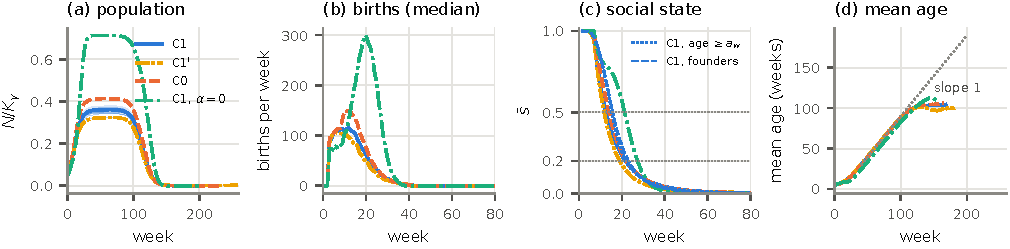
\includegraphics[width=\textwidth]{fig_res_trajectories.pdf}
  \caption{Time course of the reference ensemble ($n=200$ each).
  \textbf{(a)}~Population relative to the damage-threshold capacity $K_\gamma=m_c|G|$: median and 10--90\% band for
  \textsf{C1} (thin lines are 12 individual runs), and medians for \textsf{C1}$'$, \textsf{C0} and the $\alpha=0$
  control.
  \textbf{(b)}~Weekly births (median).
  \textbf{(c)}~Mean social state $\bar s$ of the adults (age $\ge6$ weeks; solid and dashed coloured lines as in a),
  median over living colonies, shown while at least half of the colonies are alive, on a linear scale; for
  \textsf{C1} also the mean over the animals past the plasticity window (age $\ge a_w$, dotted) and over the
  founders (dashed), which are not diluted by the newborn pups. The dotted grey lines mark the 0.5 level of O10 and
  the 0.2 deterioration threshold.
  \textbf{(d)}~Mean age, with a reference line of slope one: after natality stops, the colony simply ages.}
  \label{fig:res-trajectories}
\end{figure}

\subsection{Which patterns carry evidence: null models}
\label{sec:res-null}

A criterion is informative only if it can fail. Table~\ref{tab:res-null} gives the pass rate of every essential
pattern in four null models run from the initial condition of \textsf{C1} ($n=200$): no crowding damage
($\gamma=0$), full inheritance without social learning ($-$R2$^*$: $w=1$, individual recovery at $r=0.01$), the
long-lived demography without new rules, and \textsf{C1} without its four rules; and in the two partial ablations of
the reference ensemble ($\alpha=0$ and \textsf{C0}); Table~\ref{tab:res-null-full} (appendix) adds the desirable
patterns. NA counts as a failure. By the rule fixed before the runs, a criterion is \emph{generic} if it passes
($f\ge0.8$) in at least two of the four null models, and it \emph{discriminates} against a model if the upper
Wilson bound of its pass rate there is below 0.8 and the Newcombe interval of the difference with \textsf{C1}
excludes zero.
O5, O6, O7 and O10 are generic (they pass in three or four null models), and so is the primary O4, which still
passes in $-$R2$^*$ and without rules (the free space at the peak needs no rule: $f_0=0.74$ without rules, 0.59 in
the long-lived control; and $f_0$, part of the primary O4, was an informal target of the calibration): these five criteria
carry no evidence for the rules; they verify that the model has a boom, an end of natality and an extinction. Scored at six weeks, as in the primary evaluator, the
primary O11 discriminates against every null model, but not at the end of the plasticity window (below); O13 and
O13p discriminate against three of the four, but not
against $-$R2$^*$, where both deteriorated classes form by full inheritance without social learning (O13p 1.00
there), and O13p also discriminates against both partial ablations. O17p fails in every null model and in both
partial ablations; which criteria carry that evidence depends on the age at which O11 is scored (below). With the preregistered evaluator O10 passed in every null model
and O11 passed vacuously without crowding damage, which is why both were redefined (Table~\ref{tab:res-null-v1}).
O11 is in part definitional, because pups are born at $s=0$ and are scored at six weeks of age, inside the
plasticity window. Re-scoring the same runs with the late cohorts measured at the age $a_w=12$ instead (same
thresholds; \texttt{results\_v2/o11\_aw}), \textsf{C1} and \textsf{C1}$'$ barely change (O11 0.995 and 0.935, O17p
0.990 and 0.815), but O11 then also passes in 0.81 of the long-lived runs and in 0.755 of the runs without rules,
whose late cohorts fall below 0.2 through accumulated crowding damage, so it no longer discriminates against those
two null models; against $-$R2$^*$ it passes in 0.21 (O17p 0.205), and without crowding damage it stays NA. Their late cohorts even end lower than those of \textsf{C1} (median $\bar s$ 0.074 in the long-lived runs and
0.055 without rules, against 0.130). The dependence on $s_{\rm base}$ almost disappears at that age (below). At six
weeks, then, O11 separates \textsf{C1} from the null models largely through the birth state of the pups
($w=0.2$, $s_{\rm base}=0$; with $s_{\rm base}=0.25$ it falls to 0.08), not through a failure that the rules add to
the crowding damage, and the evidence of O17p against the long-lived
demography and the model without rules rests on O13 and O13p; against $-$R2$^*$ it rests on O11 at six weeks and is
weaker at $a_w$. O10b, the functional growth phase, passes only where crowding is absent or weak and fails in
\textsf{C1} with the adult mean (0.28 when measured on the animals past the window).

\begin{table}[t]
\centering
\caption{Discriminating power of the essential criteria (primary evaluator; fraction of all runs that pass, NA
counting as failure). Columns: the reference ensemble (\textsf{C1}, \textsf{C1}$'$, $\alpha=0$, \textsf{C0}), the
four null models with the initial condition of \textsf{C1} ($\gamma=0$; $-$R2$^*$: $w=1$ without social learning;
long-lived control; no rules: \textsf{C1} without its four rules), $n=200$ each, and the short-lived control
($n=100$). ``Generic'': passes in at least two of
the four null models. ``Discriminates'': upper Wilson bound below 0.8 and Newcombe interval of the difference with
\textsf{C1} excluding zero (long: long-lived control; none: no rules; short: short-lived control). O10b (functional growth phase) is
listed because its failure in \textsf{C1} is discussed in the text. O11 is scored at six weeks of age, as in the
primary evaluator. Scored at the end of the plasticity window ($a_w=12$; same runs, \texttt{results\_v2/o11\_aw}) it
passes in \textsf{C1} 0.995, \textsf{C1}$'$ 0.935, $\gamma{=}0$ 0.00 (NA), $\alpha{=}0$ 1.00, \textsf{C0} 0.99,
$-$R2$^*$ 0.21, long 0.81 [0.75, 0.86] and none 0.755 [0.69, 0.81] (short-lived control not re-scored): it is then not
generic (it passes in one null model) and discriminates only against $\gamma{=}0$ and $-$R2$^*$. The desirable
patterns are in Table~\ref{tab:res-null-full}.}
\label{tab:res-null}
\footnotesize
\setlength{\tabcolsep}{3.2pt}
\begin{tabular}{@{}lccccccccccl@{}}
\toprule
& \textsf{C1} & \textsf{C1}$'$ & $\gamma{=}0$ & $\alpha{=}0$ & \textsf{C0} & $-$R2$^*$ & long & none & short & generic & discriminates against \\
\midrule
O4 & 1.00 & 1.00 & 0.00 & 0.00 & 1.00 & 0.99 & 0.17 & 1.00 & 0.87 & yes & $\gamma{=}0$, $\alpha{=}0$, long \\
O5 & 0.99 & 0.85 & 1.00 & 1.00 & 1.00 & 0.97 & 0.89 & 0.91 & 0.25 & yes & short \\
O6 & 1.00 & 1.00 & 0.00 & 1.00 & 1.00 & 1.00 & 0.99 & 1.00 & 0.45 & yes & $\gamma{=}0$, short \\
O7 & 1.00 & 0.99 & 0.00 & 1.00 & 1.00 & 1.00 & 0.99 & 1.00 & 0.47 & yes & $\gamma{=}0$, short \\
O10 & 1.00 & 1.00 & 0.00 & 1.00 & 1.00 & 1.00 & 1.00 & 1.00 & 1.00 & yes & $\gamma{=}0$ \\
O11 & 1.00 & 0.97 & 0.00 & 1.00 & 1.00 & 0.00 & 0.00 & 0.00 & 0.00 & no & $\gamma{=}0$, $-$R2, long, none, short \\
O13 & 1.00 & 1.00 & 0.00 & 1.00 & 0.92 & 1.00 & 0.00 & 0.00 & 0.00 & no & $\gamma{=}0$, long, none, short \\
O13p & 1.00 & 1.00 & 0.00 & 0.00 & 0.00 & 1.00 & 0.00 & 0.00 & 0.00 & no & $\gamma{=}0$, $\alpha{=}0$, C0, long, none, short \\
O17p & 0.99 & 0.83 & 0.00 & 0.00 & 0.00 & 0.00 & 0.00 & 0.00 & 0.00 & no & $\gamma{=}0$, $\alpha{=}0$, C0, $-$R2, long, none, short \\
\midrule
O10b & 0.02 & 0.01 & 1.00 & 1.00 & 0.18 & 0.05 & 0.20 & 0.12 & 1.00 & no & none \\
\bottomrule

\end{tabular}
\end{table}


\subsection{Rule ablations and the minimal candidate}
\label{sec:res-ablations}

Fig.~\ref{fig:res-ablations} (appendix) removes the rules of \textsf{C1} singly, in pairs, in triples and all
together; each single ablation fails in a specific way. \emph{Without R7} the colony is Calhoun-like in the
instantaneous sense (O17 in 0.94), but the isolated class is never persistent (O17p $=0$). \emph{Without R2} (full
inheritance and individual recovery) the late cohorts do not fail at six weeks (O11 and O17p in 0.00 [0, 0.03]; 0.17 with the
preregistered O11, which passed when the late cohorts were empty). \emph{Without R1} adults recover when the colony
thins: natality resumes, only 23\% of the colonies go extinct by week 600, and O17p is 0.21 [0.15, 0.29].
\emph{Without AV} O17p falls to 0.79 [0.71, 0.85], through O5. Every double, triple or quadruple ablation has O17p
$=0$, and without crowding damage ($\gamma=0$) every colony grows to the cap of 15\,000 individuals. Inheritance is
not needed: with $w=0$ and a faster learning rate $r=0.15$, O17p is 1.00, so social learning is the essential part of
R2. R7 depends on its implementation and on the update scheme: without a preference ($\pi=0$) the refuges stay empty
and O17p is 0; with a soft capacity under synchronous moves O17p is also 0, because simultaneous moves send many
deteriorated animals into the same refuge, whereas under a random sequential update a soft capacity gives the same
result as the hard one (0.995 against 1.00): the hard capacity is a remedy for the collisions of the synchronous
update, not a mechanism of its own (Appendix~\ref{app:res-ablations}).

\paragraph{Q2 and the minimal candidate \textsf{C1}$'$.}
The preregistered intersection--union test is the largest of the four one-sided Fisher $p$-values, and it comes
from AV. With the primary evaluator $p_{\rm IUT}=1.1\times10^{-7}$, $p_{\rm Holm}=2.2\times10^{-7}$, so the null
hypothesis that some rule can be removed without loss is rejected; with the preregistered evaluator the
same runs give $f(-{\rm AV})=0.90$ and $p_{\rm Holm}=0.067$, not rejected, which replicates the borderline result of
the runs of the preregistered design ($p_{\rm Holm}=0.0503$). The rejection is therefore a consequence of the primary O5 alone, and specifically
of its birth reference $t_{B99}$: that option was adopted after exploratory runs with the primary evaluator had
shown that the alternative, the last sustained birth combined with $t'_{\rm pk}$, fails O5 in half of the
\textsf{C1} runs (0.48 in the production runs, Table~\ref{tab:res-rescoring}); it is a choice informed by the result
(Table~\ref{tab:deviations}), and O5 is a generic criterion (Section~\ref{sec:res-null}). The rejection of Q2 thus
shows an effect of AV on a generic criterion, significant but smaller than predicted: with either evaluator the
prediction $f(\textsf{C1}-r)\le0.5$ fails for AV (0.79), and the necessity of AV, as defined in the plan, is refuted.
The difference with \textsf{C1} is 0.20 [0.13, 0.28] in the factorial ($n=120$ per arm) and 0.16 [0.11, 0.22] in
the reference ensemble (Newcombe intervals). AV is a contributing rule: it makes the end of natality sharper (O5,
through a shorter tail of births) and supplies the senescent decline (O8 0.62 against 0.21), while it \emph{reduces}
the empty space at the peak ($f_0=0.16$ against 0.52), which is present without any rule. In \textsf{C1}$'$, R1, R2
and R7 remain necessary (O17p of 0 without each, $n=40$; Table~\ref{tab:res-c1p}).
\textsf{C1}$'$ is the minimal set \emph{conditional} on the evaluation thresholds. Re-scoring the stored class
fractions (Fig.~\ref{fig:res-theta}), O17p of \textsf{C1}$'$ is 0.83 for class thresholds $\theta\le0.125$ and 0.33
at $\theta=0.15$ (0.31 in the $-$AV arm of the factorial, $n=120$); that of \textsf{C2} falls from 0.70 to 0.01 at
0.125; \textsf{C1} holds 0.96 at 0.15. On the grid of
class and ensemble thresholds $(\theta,\tau)$, AV is ``necessary'' exactly when $\tau\ge0.8$ at $\theta\le0.125$ (0.79
lies below 0.8, with an interval that contains it) or when $\theta\ge0.15$; R1, R2 and R7 are necessary everywhere.
The necessity of R7 is necessity for O13p, a criterion designed together with R7 after \textsf{C0} had been seen;
for O11, O6 and O7 removing R7 changes nothing (O17 in 0.94).

\subsection{Confirmatory tests Q1--Q7}
\label{sec:res-Q}

Table~\ref{tab:res-Q} summarises the confirmatory family with the primary evaluator; Table~\ref{tab:res-Qcmp}
repeats it with the preregistered evaluator. With the primary evaluator six
of the seven null hypotheses are rejected after Holm adjustment and the quantitative predictions are met for Q1, Q3,
Q4 and Q7 and not for Q2, Q5 and Q6; with the preregistered evaluator five are rejected and four predictions hold
(Q3, Q4, Q6 and Q7). The two counts differ in three places: Q2 is rejected only with the primary O5 (below), the
prediction of Q1 holds only at the earlier transplant time $1.75\,t'_{\rm pk}$, and the prediction of Q6 holds only
with the preregistered O11. Q5 is refuted in the opposite direction with both. Of the predictions that hold, Q1 is a
consistency check of R1 and Q4 of the demography, and the contrast of Q3 with the short-lived control is confounded by the
demography. A rejected null hypothesis is not the same as a Calhoun-like outcome, as Q7 shows.

\begin{table}[t]
  \centering
  \caption{Preregistered confirmatory family with the primary evaluator (hypotheses and tests in
  Section~\ref{sec:stats}; Holm correction at $\alpha=0.05$ over seven tests; the $p$ of Q6 is the quasi-binomial
  one). ``Rejected'' refers to the null hypothesis after Holm adjustment; ``Met'' to the quantitative prediction
  fixed before the runs. $X$ is the cross-transplant arm. The same family with the preregistered evaluator is in
  Table~\ref{tab:res-Qcmp}.}
  \label{tab:res-Q}
  \footnotesize
  \setlength{\tabcolsep}{4pt}
  \begin{tabular}{@{}lp{4.0cm}p{5.4cm}llcc@{}}
    \toprule
    & Prediction & Estimate & $p$ & $p_{\rm Holm}$ & Rejected & Met \\
    \midrule
    Q1 & $P_T(\mathrm{D}\mid\textsf{C1})\le0.05$, $P_T(\mathrm{D}\mid X)\ge0.25$ & 0/60 vs.\ 51/60 ($P_T=0.85$ [0.74, 0.92]); discordant pairs 51:0 & $4.4\times10^{-16}$ & $1.3\times10^{-15}$ & yes & yes \\
Q2 & $f(\textsf{C1})\ge0.9$, $f(\textsf{C1}-r)\le0.5\ \forall r$ & 0.99 vs.\ $-$R1 0.21, $-$R2 0.00, $-$AV 0.79, $-$R7 0.00 & $1.1\times10^{-7}$ & $2.2\times10^{-7}$ & yes & no \\
Q3 & $P_{\rm ext}\ge0.99$, CV $\le0.10$; short-lived $\le0.7$ & 200/200 vs.\ 47/100; CV 0.066 [0.059, 0.071] & $<10^{-16}$ & $<10^{-16}$ & yes & yes \\
Q4 & slope $\in[0.8,1.25]$, $|\bar r|\le10$ wk & slope $0.996\pm0.014$; $\bar r=-2.0\pm0.3$ wk & $<10^{-16}$ & $<10^{-16}$ & yes & yes \\
Q5 & $b_2<0$, CI of $n^*_{\rm opt}\subset[4,12]$ & $b_2=+185.3\pm64.3$ (convex); no interior maximum & 1.00 & 1.00 & no & no \\
Q6 & $0<\theta<1$ & $\hat\theta=-0.15$ [-0.20, -0.05] (quasi-binomial, $\phi=3.1$) & $<10^{-16}$ & $<10^{-16}$ & yes & no \\
Q7 & corner $\ge0.8$, \textsf{C1} $\le0.2$ & 120/120 vs.\ 0/30 (30/30 explode) & $<10^{-16}$ & $<10^{-16}$ & yes & yes \\
\bottomrule

  \end{tabular}
\end{table}

\paragraph{Q1 and the transplants.}
Four males and four females of each \textsf{C1} colony, taken at $1.75\,t'_{\rm pk}$ (week 60; ages 37--64), never
found a colony in a \textsf{C1} enclosure (0/60), but do in 51/60 trials in an enclosure without R1 and R2 with
$r=0.1$ (arm $X$; exact McNemar $p=4\times10^{-16}$); the prediction ($\ge0.25$ in $X$) holds. The same animals have
$s\approx0$ (median 0.000, maximum 0.36) and fecundity scales as $s_f^2s_m$, so under R1 they cannot found a colony
with any partner (0/120 with healthy partners): a consistency check of R1, not a finding about the mechanism. The
rate in arm $X$ is a matter of age: at $1.75\,t_{\rm pk}=$ week 97 (preregistered protocol; ages 59--80) the same
colonies give 12/60, and at week 95 in every arm, the common time that removes the confound between rule and
sampling time, 5/60 (Appendix~\ref{sec:res-transplant}). An additional arm samples adults past the plasticity window with
$0.2\le s\le0.5$ (median 0.36, weeks 8--11): under R1 they found a colony in 5/60 trials, against 57/60 for the same
animals in arm $X$ and 50/60 without R1, and in the colonies they do found the adult descendants settle at the
social state of their parents (0.28--0.45 in \textsf{C1}, 0.33--0.37 in $X$). By the rule fixed in advance they
recover partly: the irreversibility of R1 + R2 is strict only for $s\approx0$, and for intermediate animals R1
acts through fecundity, not through the lineage.

\paragraph{Q3 and Q4.}
\textsf{C1} went extinct in 200 of 200 runs by $T=600$, against 47 of 100 runs of the short-lived control by $T=1000$ (one-sided
Fisher $p<10^{-16}$), with a coefficient of variation of $T_{\rm ext}$ of 0.066 [0.059, 0.071], as predicted. The
contrast that isolates the rules is the long-lived demography alone, which goes extinct in 0.98--1.00 of the runs
($p=0.11$): extinction does not discriminate. The Kaplan--Meier interquartile range over the median of
$T_{\rm ext}$ is 0.089 [0.071, 0.105] in \textsf{C1}, 0.160 [0.144, 0.180] in the long-lived control with the same
initial condition and 0.121 [0.106, 0.148] in \textsf{C1}$'$, whose difference from the control, $-0.040$
[$-0.065$, $-0.006$] (percentile bootstrap over runs), is \emph{not} within the preregistered equivalence margin of $\pm0.05$, which the runs of the preregistered design had met. A narrow
spread is not a signature of the rules (0.045 without attraction, 0.084 in \textsf{C0}): it is set by how abruptly
natality stops and by the lattice size (below). The time from the last birth to extinction grows one-to-one with
$a_{\max}$ (slope $0.996\pm0.014$ over 300 runs, TOST $p<10^{-16}$), as the demography requires
(Eq.~\eqref{eq:phaseD}; Appendix~\ref{app:res-Q}).

\paragraph{Q5 and Q6.}
The coexistence band predicted at $n^*=1/\kappa-1/\alpha\approx m_c$ (Eq.~\eqref{eq:model-nstar}) is refuted:
O13 passes in at least 95\% of the runs at 46 of the 49 points of the $(\alpha,\kappa)$ plane with $n^*>0.5$, and
the fitted quadratic in $\log n^*$ is convex; with refuges the isolated class no longer depends on the balance
between attraction and aversion. The prediction of Q6, $0<\theta<1$ for the Calhoun-like boundary in
$\log r+\theta\log a_w$ on the plane $(r,a_w)$, is not supported with the primary evaluator. The boundary is nearly
vertical in $r$: O17p is at least 0.67 for $r\le0.10$ and at most 0.60 for $r\ge0.2$ at every window, so the window
has little or no effect, and the single-index fit gives $\hat\theta=-0.15$ [$-0.20$, $-0.05$] (profile likelihood,
quasi-binomial correction $\phi=3.1$) in a model that an additive one beats ($\Delta{\rm QAIC}=28$); with the
preregistered evaluator the single-index model is the preferred one ($\Delta{\rm QAIC}=11$ in its favour) and gives
$\hat\theta=0.30$ [0.15, 0.50], as in the runs of the preregistered design (0.35). The small negative value should not be read as a reversal of
the predicted dependence: it comes from the primary O11, which at fast learning ($r\ge0.2$) fails more often the
shorter the window (O11 passes in 0.10 of the runs at $r=0.2$ with $a_w=4$ and in 0.87 with $a_w=24$), and the
change of criterion also changes which model fits the plane. The elasticity argument of
Section~\ref{sec:meanfield} does not describe this plane.

\paragraph{Q7: endogenous collapse without crowding, and the dependence on $\Lambda=r\,a_w$.}
With crowding damage switched off ($\gamma=0$), the four subcritical points ($w\le0.1$, $r\le0.03$) went extinct in
120/120 runs, while all 30 \textsf{C1} colonies exploded (one-sided Fisher $p<10^{-16}$); the colonies of the corner
first overshoot the damage-threshold capacity ($\rho_{\rm pk}=0.91$--$1.60$), so none is Calhoun-like. With
$a_w\in\{6,12,24\}$ varied at $\gamma=0$ (54 points, 20 runs each; Fig.~\ref{fig:res-q7aw},
Table~\ref{tab:res-q7aw}), 51 of the 54 points have $P_{\rm ext}=0$ or 1, so the logistic model in
$\log r+\theta\log a_w$ fixed before the production runs is separated: its profile intervals and likelihood ratio measure the
geometry of the grid, not sampling error, and the planned equivalence test of the two exponents (TOST, margin
$[2/3,3/2]$) cannot be carried out as inference (Appendix~\ref{app:res-Q}). What the design does establish is
non-parametric. The transition in $\Lambda=r\,a_w$ is bracketed by two adjacent grid points, a factor 1.25--1.5
apart; at every inheritance weight the curves for $a_w=12$ and 24 lie in the same bracket and the curve for $a_w=6$
one grid step below ($\Lambda_{1/2}\in(0.60,0.84)$ against $(0.84,1.2)$ at $w=0$; log-linear interpolation 0.71,
0.99 and 1.00). The exponent implied between windows is therefore in $(0,1)$ between 6 and 12 weeks (interpolated
0.5--0.7 over the three $w$) and compatible with 1 between 12 and 24 weeks (interpolated 0.88--1.00), where the grid
bounds it only within about $(0.5,1.5)$. The firm result is qualitative: at equal product $r\,a_w$ the six-week
window is less effective, so a single exponent does not describe the three windows and the effective learning grows
less than linearly with the window at short windows. The boundary fitted as $\sigma w+\varphi\Lambda=1$ gives
$\hat\varphi\approx1.1$--1.2 in both planes, above the preregistered $\varphi\le1$, but it is an extrapolation of the
same separated predictor and carries no valid interval.

\subsection{Robustness}
\label{sec:res-robustness}

\paragraph{Demographic and update variants, and the initial condition.}
Fig.~\ref{fig:res-rob} and Table~\ref{tab:res-rob} report \textsf{C1} and \textsf{C1}$'$ under the robustness variants
($n=200$ each), scored with both evaluators and also with O17p restricted to the criteria
that discriminate against the null models (O11 scored at six weeks, O13, O13p and the anti-patterns); by the rule fixed before the runs, a
variant preserves the result if O17p $\ge0.8$. With a constant background hazard $\mu_{\rm bg}$ at all ages the
plateau shrinks (51 weeks at 0, 35 at 0.001, 17 at 0.003 and 10 at 0.008 per week) and O17p falls to 0.83, 0.63,
0.55 [0.48, 0.62] and 0.06 in \textsf{C1} (0.67, 0.38, 0.28 and 0.04 in \textsf{C1}$'$; 0.45 at 0.003 with the
preregistered evaluator). The only criterion that fails is O5, and it fails through its timing clause, not through its
level: at $\mu_{\rm bg}=0.003$ O5 is marginal in 83 of the 200 runs and fails in 7, because the start of the plateau
$t'_{\rm pk}$ moves from week 34 to 29 while $t_{B99}$ moves from 40 to 43, so $(t_{B99}-t'_{\rm pk})/t'_{\rm pk}$
crosses the 0.5 threshold of O5 while natality still ends with the population near its maximum; at
$\mu_{\rm bg}=0.008$ O5 fails outright in 70 runs (marginal in 118). The classes, O11 and the low peak are
unchanged, and the restricted outcome is 1.00 at every $\mu_{\rm bg}$. Since O5 is generic (Section~\ref{sec:res-null}),
what the background mortality removes is the generic part of the primary outcome, not the part that carries
evidence for the rules; the primary outcome as defined nevertheless holds only without, or with very weak,
background mortality, which is stated as a limitation (Section~\ref{sec:limitations}). With initial ages drawn
uniformly from 4--52 weeks instead of all equal, O17p is 0.93 [0.89, 0.96]; from 4--80 weeks, which includes
post-reproductive founders, 0.63 [0.56, 0.69] (0.68 and 0.31 in \textsf{C1}$'$), again through the timing clause of
O5 (73 marginal and 1 failed of 200; plateau 28 and 22 weeks, $t'_{\rm pk}$ at weeks 30 and 29) and with the
restricted outcome at 1.00. The timing of the end of natality relative to the start of the plateau is therefore a
property of the synchronous initial condition and of the absence of background mortality, not of the rules; the end
of natality near the maximum itself persists. The other variants preserve the result: a nest period of three weeks
gives 0.835 [0.78, 0.88], borderline because the interval contains 0.8 (0.60 in \textsf{C1}$'$; O11 0.90,
$\rho_{\rm pk}=0.31$); a random sequential update gives 1.00
with the hard and 0.995 with the soft capacity, with $\rho_{\rm pk}=0.43$; and the exact
refuge capacity gives 0.995 against 0.995 with the single-pass admission. Pups born above the
deterioration threshold ($s_{\rm base}=0.25$ or 0.5 instead of 0) give O17p of 0.08 and 0.00 (0.64 and 0.36 with
the preregistered O11), entirely through O11 scored at six weeks of age: the failure of the late cohorts at that age is
partly definitional, tied to $s_{\rm base}=0$. Scored at the age $a_w$, the same runs give O11 of 0.975 and 0.785
and O17p of 0.965 and 0.76 (0.755 and 0.77 in \textsf{C1}$'$): by the end of the window the late cohorts are below
0.2 whatever their birth state, through crowding damage and learning from deteriorated neighbours.

\paragraph{Lattice size, seeding density and phase planes.}
Over $L=15$--60 at fixed density $N_0/L^2=0.44$ ($n=60$; Table~\ref{tab:res-size}), the peak density (0.35--0.37)
and the persistent fraction (0.17--0.18) do not change, the empty fraction decreases slightly (0.18 to 0.15), and
O17p rises from 0.82 [0.70, 0.89] at $L=15$ to 1.00 at $L\ge45$; the losses at $L\le20$ come from O5 (5 of 60 runs
at each size: a relatively longer tail of births with $N_0=100$--178), from O11 (1 of 60 at each) and, at $L=15$
only, from the anti-pattern A2, a recovery of natality in 6 of 60 runs, and the interval at $L=15$ contains 0.8.
The spread of the extinction time falls from 0.15
at $L=15$ to 0.08 at $L\ge30$ together with the relative spread of the last birth (0.58 to 0.18), while
$T_{\rm ext}-t_{\rm last}$ stays at 110--112 weeks: the spread of $T_{\rm ext}$ is that of the end of natality, as
Eq.~\eqref{eq:phaseD} implies, and its value is a property of the system size. Over seeding densities from 0.02 to
3.6 animals per cell the peak density is monotone in $N_0/L^2$ and O17p reaches 0.8 only for
$0.2\lesssim N_0/L^2\lesssim0.9$; with Calhoun's four founding pairs no run is Calhoun-like, and the best point of
the founder plane reproduces O1--O3 with O17p in 0.43 [0.27, 0.61] of the runs (Appendix~\ref{app:res-p4p6}).
Around \textsf{C1} the primary outcome holds over part of the explored planes (Appendix~\ref{sec:res-planes}): with
crowding damage every point of the $(r,w)$ plane goes extinct and O17p is at least 0.83 for $w\le0.3$ and
$r\le0.10$, falling at $w\ge0.5$ and $r\ge0.2$ through O11; every finite window $a_w\le24$ gives certain
extinction; in the $(\alpha,\kappa)$ plane O17p is at least 0.8 at 34 of the 48 points with $\alpha\ge2$, failing
where the free space of the primary O4 is lost; and a persistent isolated class requires a strong preference and a
total refuge capacity $f_Rc_R\ge0.4$. These are point estimates with 30 runs per cell (Wilson half-width up to
$\pm0.17$); re-running the 40 points nearest to a boundary with 100 runs changed them by 0.07 on average.

\paragraph{Global: Latin hypercubes and variance decomposition.}
Over two independent 15-factor Latin hypercubes (400 points, 10 runs each, plus 40 runs at the 18 points near the
boundary), 2.0\% [0.7, 3.6] of the points are Calhoun-like with the primary evaluator ($k/n\ge0.8$; bootstrap
interval over points); the mean of O17p over the box, an unbiased estimate of the volume weighted by the
probability of being Calhoun-like, is 4.0\% [2.6, 5.9], and the empirical-Bayes fraction of points with $p\ge0.8$,
which shrinks each point towards a logistic emulator, is 1.8\% [0.7, 3.2], with 8 points still uncertain
(Table~\ref{tab:res-region}, Fig.~\ref{fig:res-region}). With the preregistered evaluator the same runs give 7.2\%,
11.0\% and 6.9\% [4.8, 9.2], the values of the runs of the preregistered design; the drop comes mostly from O5 with $t'_{\rm pk}$ and from the
free-space condition of O4. Every such fraction is relative to the box and to the sampling scales of
Table~\ref{tab:params}. Part of the small fraction is definitional and part is mechanism: with $c_R=3$ refuge
residents exceed the isolation threshold and none of the 100 such points is Calhoun-like; restricting successively
to $c_R\le2$, $m_c\le10$, $f_Rc_R\ge0.3$ and $\pi\ge100$ (chosen after the runs) raises the fraction to 2.7\%, 3.1\%,
5.6\% and 10.8\% [2.7, 21.6] (4 of 37 points; 46\% with the preregistered evaluator), and even then 33 of the 37 points
fail, through O11 (16), the persistence of the class (14), O5 (9) and O4 (9); with class thresholds of 5\%, 10\% and
15\% the fraction is 5.5\%, 2.3\% and 0.5\%. The Sobol' decomposition uses 11 factors (the 8 selected by the Morris
screening plus $w$, $r$ and $a_w$; Saltelli design, $N=256$, 6 runs per point), so its indices are conditional on
four factors held at their \textsf{C1} values ($f_R$, $\pi$, $a_{\max}$, $\delta$). O17p is zero at 78\% of its
points; its total indices are led by $c_R$ ($0.49\pm0.16$), $w$ (0.43), $\kappa$ (0.41), $r$ (0.32) and $m_c$ (0.31),
which cannot be ordered, and its first-order indices add up to only 0.15, so it is almost entirely interactions;
the continuous outputs are nearly additive ($\rho_{\rm pk}$: $r$, $\kappa$, $\eta$, $\gamma$; $f_0$: $\kappa$, $m_c$;
$\Phi^{\rm pers}_{\rm BO}$: $c_R$, $m_c$). Appendix~\ref{sec:res-sensitivity} gives the full decomposition.

\section{Discussion}
\label{sec:discussion}

\paragraph{The envelope is generic; the rules add the classes.}
The main lesson of the production runs is a negative one.
A long-lived demography alone, without any of the new rules, drives nearly every colony to extinction (98/100 in the long-lived control, 199/200 in the corresponding null model run from the initial condition of \textsf{C1}).
Once natality stops, the colony simply ages out, and the phase-D law Q4 is a consistency check of that demography.
Extinction is therefore \emph{not} a result of the rules, and neither is the rest of the envelope: with crowding
damage and the calibrated attraction $\alpha=4$, the candidate without its four rules has a low peak with free space,
an end of natality near the maximum and no rebound (Table~\ref{tab:res-null}), and, scored at the end of the
plasticity window, late-born cohorts that fail to acquire social competence.
We distinguish what the rules encode, what they add, and what the demography and the initial condition set.

\paragraph{Consistency checks of the design.}
Several patterns follow from the rules by construction; they verify the implementation, but they are not findings.
\begin{itemize}
\item \emph{Transplants (O12, O12b, Q1).} Under R1 an adult cannot recover, and conception and pup survival scale
  with the social state of the parents. Phase-D animals have $s\approx0$ (median 0.000 in every arm with R1;
  Table~\ref{tab:res-trans-s}), so they cannot found a colony, with healthy partners or without them (0/60 and 0/120
  in \textsf{C1}). R1 was motivated by Marsden's transplants \cite{Calhoun1973}, and the cross-transplant arm only
  shows that removing the ratchet restores recovery. The non-trivial part is upstream: that the colony drives
  essentially every adult to $s\approx0$, which O10 and O11 measure and which crowding damage alone largely
  achieves. Adults of intermediate social state
  ($0.2\le s\le0.5$, which exist only around weeks 8--20) found a colony in 5 of 60 trials under R1, against 57 of
  60 without R1 and R2: the ratchet also blocks them, through their fecundity, but where they do found a colony
  their offspring settle at the parents' level ($\bar s\approx0.3$--0.4) and the lineage does not collapse
  (Appendix~\ref{sec:res-transplant}).
\item \emph{Persistence of the isolated class (O13p).} R7 was designed after the first candidate produced only a
  transient isolated class, and its capacity $c_R=2$ equals the isolation threshold of O13.
\item \emph{Senescent decline and no social deaths (O8, A4).} Social mortality is off in every preset.
\end{itemize}
Table~\ref{tab:res-null} gives the pass rate of each essential pattern in the null models; the patterns above are
marked $^\ddagger$ in Table~\ref{tab:observations}, whose caption names the rule that implies each of them.

\paragraph{What the rules add.}
Of the eight essential criteria of Table~\ref{tab:res-null}, five (O4, O5, O6, O7 and O10) pass in at least two of
the four null models and carry no evidence for the rules: they verify that the model has a boom, an end of natality
and an extinction. In particular the low peak with free space is generic: the candidate without its four rules
passes the primary O4 in 200 of 200 runs ($\rho_{\rm pk}=N_{\rm pk}/K_\gamma=0.45$, $f_0=0.74$), and the long-lived
control fails it only through its high peak ($\rho_{\rm pk}=0.85$), not through a lack of free space ($f_0=0.59$).
$K_\gamma=m_c|G|$ is the population at which every cell would sit at the damage threshold, not a physical capacity.
What the rules add, and the null models lack, is two patterns:
\begin{itemize}
\item \emph{Coexisting crowded and isolated deteriorated classes} (O13). They are absent in the long-lived control,
  without crowding damage and without the rules, and present with crowd aversion or refuges alone (1.00 in
  \textsf{C1}$'$, 0.92 in \textsf{C0}); full inheritance without social learning also has them. This is a
  calibrated property, obtained in a nearly sessile regime (below), and it is lost with more movement sub-steps.
\item \emph{The persistence of the isolated class} (O13p), which discriminates against three of the four null models
  but holds by design ($c_R=2$ equals the isolation threshold).
\end{itemize}
The failure of the cohorts born during the boom (O11) is not among them. Scored at sexual maturity (six weeks), as
in the primary evaluator, O11 passes in 1.00 of the \textsf{C1} runs against 0.00 in each null model and needs R1
and R2 (0.71 of the applicable runs and 0.00 without each), but that separation was partly definitional: pups are born with
$s\le w\,s_f\le0.2$, the threshold that O11 uses, and at six weeks they are still inside the plasticity window, so
with pups born above the threshold ($s_{\rm base}=0.25$ or 0.5) O11 failed and O17p dropped to 0.08 and 0.00.
Scored at the end of the window ($a_w=12$ weeks) on the same runs, \textsf{C1} still passes (O11 0.995, O17p 0.990),
the dependence on $s_{\rm base}$ disappears (O17p 0.965 and 0.76), and O11 also passes in 0.81 of the long-lived runs
and in 0.755 of the runs without rules, whose late cohorts fall below 0.2 through accumulated crowding damage. Only
against full inheritance without social learning does it still separate in part (0.21). The failure of the late
cohorts is therefore mostly the crowding damage of the envelope, not a contribution of the rules. Against the
long-lived control and the model without rules, the evidence that the primary outcome O17p carries for the rules
rests on O13, with O13p as a design property; against full inheritance without social learning it rests on O11 at
six weeks and is weaker at the end of the window. Crowd aversion is not needed for either pattern (\textsf{C1}$'$
passes them), and it does not supply the free space at the peak: it reduces it ($f_0=0.16$ with AV, 0.52 without).

\paragraph{The central limitation: demography and initial condition.}
The model has no mortality before senescence, and its default initial condition is a synchronous cohort of 400
healthy four-week-old animals. Both matter for the primary outcome. Without background mortality nobody dies until
old age, so the population sits on a plateau of about 51 weeks and $t_{\rm pk}$ is an arbitrary point of it; the ratio
$(T_{\rm ext}-t_{\rm pk})/t_{\rm pk}$ is 2.1, close to Calhoun's 1.84--2.2, with $t_{\rm pk}=\arg\max N$, but 4.0
from the start of the plateau, so we do not count it as agreement. Calhoun recorded adult deaths during phases B and
C. With a background hazard of 0.003 per week at all ages the plateau shrinks to 17 weeks and O17p falls from 0.995
to 0.55; with 0.008 per week, to 0.06. With initial ages spread over 4--52 weeks O17p is 0.93, but over 4--80 weeks it
is 0.63 (Section~\ref{sec:res-robustness}). In every case the only criterion that fails is O5, and it fails by its
timing clause, not by its level clause. Natality still ends with the population near its maximum (at the 99th
percentile of the births the population is about $0.99\,N_{\rm pk}$), but the deaths bring the start of the plateau
forward ($t'_{\rm pk}$ moves from 34 to 29 weeks at 0.003 per week, medians over 200 runs) while the end of natality
hardly moves (40 to 43 weeks), so $(t_{B99}-t'_{\rm pk})/t'_{\rm pk}$ crosses 0.5 and O5 becomes MARGINAL. This is
the case in 83 of the 90 failing runs at 0.003 per week and in 73 of the 74 failing runs with ages over 4--80 weeks;
the remaining ones, and the 70 runs that fail O5 at 0.008 per week, exceed the timing clause by more than a factor
two. O5 is generic, and the patterns that the rules add (O13 and O13p), as well as O11, pass in every run of these
arms. The
dependence on the demography and on the initial condition is therefore a dependence of the timing of the end of
natality relative to the start of the plateau, a quantity that also rests on the post hoc choice of $t'_{\rm pk}$.
It is not evidence against what the rules add, nor for it, since O5 discriminates against no null model; but it
does mean that O17p $=0.995$ overstates how robustly the full conjunction of patterns is reproduced. A nest period
of three weeks (0.835, borderline) and a random sequential update (1.00) preserve the primary outcome.

\paragraph{The dynamics is a boom and its senescence, a compressed sequence of phases.}
The time course of \textsf{C1} is essentially one transient (Tables~\ref{tab:calib-generations}
and~\ref{tab:calib-chrono}; reference ensemble, 200 runs). The founders deteriorate by crowding during their own adult
life, from $s=0.90$ at the end of the plasticity window to 0.20 at 26 weeks of age. Their offspring, about 70\% of
all births, are born below the deterioration threshold and fail to acquire competence, because competent adults have
become scarce. The net reproductive number falls from 3.8 in the founders to 0.40 in their daughters, so natality
stops within about one generation, and the third and later generations add 3.2\% of the births. The null
models without the rules have a \emph{deeper} boom: with the same attraction and crowding damage, \textsf{C1}
without its four rules has a mean generation of the births of 1.59 against 1.34 and a net reproductive number of 0.66
in the first generation against 0.40, and the long-lived control 1.95 and 1.2 (30 runs each;
Table~\ref{tab:calib-gamma}). The rules, R2 in particular ($-$R2$^*$ gives 1.62), shorten the generational depth
rather than create a long cascade.
The shallowness of the boom is set by how pups are born and socialised: they are born below the deterioration
threshold ($w=0.2$, $s_{\rm base}=0$), conception and pup survival scale with the parents' social state, and social
learning (R2) draws on adults who are already deteriorating, so the net reproductive number drops in the first
generation. A ratio of time scales gives a heuristic comparison with Universe~25, not the cause. Measured on animals
past the plasticity window, so that newborns do not dilute it, $\Gamma=t_{\rm det}/T_{\rm gen}$ is
$\approx1.1$ (1.2 on the founders; about 0.7 if $T_{\rm gen}$ is taken as the mean age of the mothers at birth,
14.3 weeks, so it is of order one under either definition); in Universe~25 the ``death of societal organization'' took the whole of phase~C, about 35
weeks, with a generation time of about 10 weeks, so $\Gamma\approx3.5$, an order of magnitude with a different
operational definition. The model has a growth phase with
socially competent adults, but it is about half as long as Calhoun's phase~B (13 against 30 weeks), although it holds two thirds
of the births, and O10b, which asks for it, passes in 0.28 of the runs when the adult mean is replaced by that of the animals
past the window (0.02 with the adult mean, which the newborns dilute). The phases appear in Calhoun's order, but B
and C are compressed and an artificial plateau precedes D.
Within this transient, crowding damage is the trigger (without it colonies explode), social learning (R2) the
amplifier, the plasticity window (R1) the ratchet and the refuges (R7) make the isolated class persistent. The
ratchet matters because of the refuges: they are pockets of low density in which, without R1, deteriorated animals
recover and breed again (natality resumes and O17p falls to 0.21), whereas without refuges the collapse stays
irreversible in most runs even without R1. R1 is what lets a persistent isolated class coexist with an irreversible
collapse (Section~\ref{sec:model-rules}). Only where
socialisation is subcritical does the learning cascade propagate over several generations and kill a colony without
crowding (Q7), and those colonies first overshoot the crowding threshold, so this is not Calhoun's collapse.

\paragraph{The timing of extinction is extreme-value statistics.}
A post hoc analysis of the runs of the preregistered design suggested that crowd aversion makes the extinction time
more reproducible. It is not a
signature of the mechanism. Without social mortality $T_{\rm ext}\approx t_{\rm last}+\ell_{\max}$, the last birth
plus the longest residual lifetime (Appendix~\ref{app:calib-evs}). The second term, about 110 weeks, fluctuates only
on the scale of the inverse slope of the senescent hazard, as expected for the maximum of many lifetimes
\cite{Gumbel1958,Coles2001}, so the spread of $T_{\rm ext}$ is that of the last birth (correlation 0.92), set by how
abruptly natality stops. Without attraction the spread is 0.04, smaller than in \textsf{C1}, and it falls with the
size of the lattice (0.14 at $L=20$, 0.08 at $L=30$--60; Table~\ref{tab:res-size}).

\paragraph{What ``minimal'' means here.}
``Minimal'' does not mean few parameters: the core model has more than a dozen, and the added rules about ten (R1: $a_w$;
R2: $\lambda$, $w$, $s_{\rm base}$; AV: $\kappa$, $p$; R7: $f_R$, $c_R$, $\pi$, $q$, $b$ and the hard capacity), all
fixed by qualitative calibration against the evaluated patterns. It means that every added rule is local, has a
neutral value that recovers the core model and is motivated by an observation in Calhoun's report; that rules
found unnecessary were removed (long-range jumps, state-dependent attraction, territorial exclusion, social
mortality); and that each rule of the minimal set is necessary by ablation \emph{at the evaluation thresholds used}:
a class threshold of 10\%, isolation at $m\le2$, persistence of four weeks and an ensemble threshold of 0.8.
The necessity of R7 is necessity for O13p, a criterion added together with R7; for O6, O7 and O11 removing R7 changes
nothing, whereas R1 and R2 remain needed (O11 in 0.71 of the applicable runs and 0.00 without each).
The preregistered necessity test Q2 is rejected with the primary criteria ($p_{\rm Holm}=2.2\times10^{-7}$) but not
with the preregistered criteria ($p_{\rm Holm}=0.067$); the rejection comes only from the post hoc choice of $t_{B99}$ in
O5, a generic criterion (Table~\ref{tab:deviations}). Removing AV lowers the primary outcome by 0.20 [0.13, 0.28] in
the factorial. The predicted size of the effect, however, fails: without AV the primary outcome was to fall to at
most 0.5, and it is 0.79 [0.71, 0.85]. AV therefore contributes but is not necessary in the preregistered sense; we
do not use the observed power of the test, which cannot explain a decision \cite{HoenigHeisey2001}.
At these thresholds the minimal set for the primary outcome is \textsf{C1}$'$ (R1, R2 and R7): 0.835 [0.78, 0.88] of
200 runs, borderline because the lower bound is below 0.8, against 0.995 for \textsf{C1} (not preregistered). It falls
to 0.33 at a class threshold of 15\%, and that of
\textsf{C2} from 0.70 to 0.01 at 12.5\% (Fig.~\ref{fig:res-theta}), so minimality is not a property of the rules
alone. Adding AV makes O5 more reliable and the decline senescent (O8 in 0.62 against 0.21), and reduces the free
space at the peak ($f_0=0.16$ against 0.52); partial inheritance is not necessary
($w=0$ with $r=0.15$ gives 1.00). Making the list of required patterns and their thresholds explicit, and testable
run by run, is in our view the main methodological contribution of this work.

\subsection{Limitations and circularity}
\label{sec:limitations}

\paragraph{Circularity between the patterns and the calibration.}
The same patterns and evaluator were used to \emph{choose} the rules and to \emph{report} them; no pattern was held
out. The refuge capacity $c_R=2$ coincides with the isolation threshold of O13 (with $c_R=3$, O17p is zero at every
point of the sensitivity designs); the persistence criterion O13p was added after \textsf{C0}, and R7 was designed to
satisfy it; $m_c$ is both the damage threshold and, in the preregistered evaluator, the boundary of the crowded class (with a fixed
threshold $m>8$ the Calhoun-like fraction of the hypercubes is 2.0\%, against 2.5\% with $m>m_c$). The empty fraction
at the peak was used informally to discard candidates and is a condition of the
primary O4; O12 was used to choose $\alpha=4$ (Section~\ref{sec:circularity}).
The fulfilment of the patterns by \textsf{C1} therefore shows that they are \emph{possible} under local rules, not
that they were predicted. Among the preregistered tests, Q1 and Q4 are consistency checks, the contrast of Q3 is
confounded by the demography, the prediction of Q6 is not supported (with the primary O11 the window has little or no
effect on the boundary), and Q7 establishes an endogenous collapse without crowding, not the form of its boundary. All deviations from the plan are listed in Table~\ref{tab:deviations}.

\paragraph{Robustness.}
Against stochasticity robustness is high: O17p is 0.995 [0.97, 1.00] over 200 runs, independent ensembles replicate
it, eight refuge layouts gave no difference, and exploratory runs on lattices up to $L=84$ at fixed
density (30 runs per size, single-pass refuge admission) give the same peak density and persistent class, with no healthy pocket reseeding the colony. Locally it holds over most of
the phase planes, whose boundaries are estimated from 30 runs per point. Globally it is limited and relative to the
sampled box: over two 15-factor Latin hypercubes the mean primary outcome is 0.040 [0.026, 0.059] and 2.0\%
[0.7, 3.6] of the points are Calhoun-like (7.2\% with the preregistered criteria). Part of this is definitional ($c_R=3$,
large $m_c$) and part is mechanism (a total refuge capacity $f_Rc_R\ge0.3$ and a strong preference $\pi\ge100$); even
with the four restrictions together, chosen after the runs, 33 of 37 points fail. The Sobol' indices are conditional
on the factors fixed after screening. Demographically, the primary outcome depends on the timing of the end of natality, as discussed above, while the
patterns that the rules add do not.

\paragraph{Scales and the comparison with Universe~25.}
With at most one Moore step per week, the Damköhler number $t_{\rm mix}/t_{\rm det}$ is about $1.7\times10^2$ in
\textsf{C1} (about 10 for founder colonies), against $\lesssim4\times10^{-3}$ in Universe~25, whose mice crossed the
enclosure every day (Table~\ref{tab:calib-scales}). The spatial structure of the model is that of animals almost
sessile on the scale of the deterioration, and with more movement sub-steps the coexistence of classes is lost. The
model lacks the separation $t_{\rm mix}\ll T_{\rm gen}\ll t_{\rm det}$ of Universe~25. We map a cell to a nest box, $m_c$ to its comfortable occupancy (``fifteen
mice could comfortably rest in a single nest box'' \cite{Calhoun1973}), $K_\gamma$ to Calhoun's 3840 places and the
refuges to the little-preferred high nests; $c_R=2$ is the isolation threshold, not the capacity of a nest. With this
mapping $f_0$ and $\rho_{\rm pk}$ have the same definitions as Calhoun's 20\% of empty nest boxes and 0.57, but $|G|$
and $m_c$ were not calibrated and $\rho_{\rm pk}$ depends on the seeding density, so they agree only in sign. R7 was
calibrated with synchronous moves; the exact hard capacity leaves the primary outcome unchanged, and with a random
sequential update a soft capacity suffices ($\rho_{\rm pk}=0.43$).

\paragraph{What is not reproduced.}
The founder phase (O1--O3): from four founding pairs a colony spreads as a slow front, and no point of an exploratory
founder plane is Calhoun-like (O17p at most 0.37). The beautiful ones (O13b): the persistent isolated class of
\textsf{C1} is made of refugees of the early boom, most of whom entered the refuges as pups, not of a late-born
cohort; the variant \textsf{C2} produces a later-born class at a demographic cost. Total infant mortality (O15) and the
sex bias of the remnant (O9) are not reproduced, because conception and pup survival decline together and there is no
sex-specific mortality. Details, the refuted coexistence band (Q5) and the comparison with
\cite{GwizdallaDus2026} are in Appendix~\ref{app:discussion}. That model reproduces the founder phase and the timing
of the curve, which ours does not; ours shows that local rules, without population-level switches, produce
coexisting classes of deteriorated animals, one of them persistent, on top of an envelope (a low peak with free
space, an end of natality and the failure of the late-born cohorts) that crowding damage and the demography already
give. Both agree that replicate variability is large and that Calhoun's trajectory is one admissible outcome among
many. We make no claim about human populations.

\paragraph{Future work.}
A founder protocol with realistic mobility and an explicit adaptation phase; patterns held out from the calibration;
gestation, lactation and background mortality, so that births spread up to the peak, which is the condition for a
late-born isolated cohort and for natality to end at high population without a synchronous start; decoupling
conception from pup survival and adding sex-specific risks; and a closer comparison with maternal-effect theories of
population cycles \cite{GinzburgTaneyhill1994,InchaustiGinzburg1998}.


\section*{Code and data availability}
All code, simulation outputs and analysis scripts are available in the repository \repourl; the version used in this paper (release v1.0) is archived in Zenodo, \zenododoi{10.5281/zenodo.23111283}. The model is implemented in the Python package
\texttt{u25}; the candidates of this paper are the presets \texttt{calhoun\_C0}, \texttt{calhoun\_C1p} (\textsf{C1}$'$),
\texttt{calhoun\_C1} and \texttt{calhoun\_C2}. Every ensemble reported here is generated by
\texttt{scripts/production/run\_2b\_v2.sh} with fixed base seeds recorded in each \texttt{results\_v2/f2b\_*/meta.json};
the confirmatory family and the remaining stages are analysed in \texttt{results\_v2/f2b\_final/}, and every number
quoted in Results is dumped, with its ensemble, to \texttt{results\_v2/results\_numbers.json}, including O11 at
age $a_w$ (re-run with the same seeds in \texttt{results\_v2/o11\_aw/}, \texttt{make o11-aw}) and $\Gamma$ (re-run in
\texttt{results/fisico\_v3/} by \texttt{scripts/analysis/gamma\_v3.py}). All figures and
tables are regenerated by \texttt{make figs}, as described in the repository README. The preregistered statistical
plan is reproduced in \texttt{docs/preregistered\_plan.md}.

\section*{Declaration of generative AI use}
The author designed the project and provided a preliminary implementation of the agent-based model, together with a
draft describing its objectives and interaction rules, which were taken as the starting point. Claude (Anthropic),
used through Claude Code in a multi-agent setting (agents with the roles of mathematician, physicist, programmer and
literature reviewer, coordinated by a principal agent), contributed to the reimplementation and extension of the
code, the simulations, the statistical analysis, the literature review and the writing of the manuscript. An
independent system of Claude agents carried out an internal review in three rounds. The author supervised the work,
reviewed all of its content and takes full responsibility for it.

\bibliographystyle{plain}
\bibliography{refs}

\appendix
\section{Model description following the ODD protocol}
\label{app:odd}

We follow the second update of the ODD protocol \cite{Grimm2020}.
Parameter names refer to the \texttt{Params} class of the \texttt{u25} package.

\subsection{Purpose and patterns}
The purpose is to identify a minimal set of \emph{local} rules that, with unlimited resources and without thresholds
on the total population, generates the qualitative sequence reported for Universe~25 \cite{Calhoun1973}:
\begin{enumerate}
\item latency;
\item exponential growth;
\item deceleration with social deterioration;
\item cessation of surviving births near the peak;
\item decline without recovery to extinction;
\item differentiated classes of deteriorated animals.
\end{enumerate}
The model is evaluated against the patterns of Table~\ref{tab:observations} and, for each pattern, against null
models (Section~\ref{sec:res-null}). With the default initial condition only items 3--6 are testable, and the model
reproduces them as a boom of one or two generations followed by extinction by senescence; of these items, the
crowding damage and the demography already give the end of natality and the decline, and the rules add the
classes of item~6 (Section~\ref{sec:discussion}).

\subsection{Entities, state variables and scales}
\begin{description}
\item[Agents (mice).] Each agent $i$ carries:
  \begin{itemize}
  \item an identifier;
  \item sex $\sigma_i\in\{M,F\}$, fixed at birth;
  \item a cell $(x_i,y_i)$ on an $L\times L$ lattice;
  \item an age $a_i$ in weeks;
  \item a social state $s_i\in[0,1]$, where $1$ means full social competence;
  \item optionally, a refractory counter and the maternal social state at birth $h_i$ (used by \textsf{C2}).
  \end{itemize}
\item[Pairs.] Each pair carries a symmetric affinity $F_{ij}\in[0,1]$, stored sparsely: only pairs with
  $F_{ij}\ge\varepsilon$ are kept.
\item[Cells.] A cell has its occupancy $n_c$, which is derived. Ordinary cells have no occupancy limit. A fixed
  random fraction $f_R$ of cells are \emph{refuges} with capacity $c_R$. The layout is drawn once with its own random
  generator (\texttt{refuge\_seed}${}=0$) and is the same in every run of every stage, so all intervals are
  conditional on it; eight alternative layouts gave no detectable
  difference.
\end{description}
\textbf{Scales.}
\begin{itemize}
\item One time step is one week.
\item The lattice has $L=30$ and hard walls.
\item A cell is an abstract meeting place, not a metric distance.
\item Mapping: a cell corresponds to a resting place (a nest box of Universe~25 \cite{Calhoun1973}), the damage
  threshold $m_c$ to its comfortable occupancy, and $K_\gamma=L^2 m_c=7200$, the population at which every cell would
  sit at the damage threshold, to Calhoun's 3840 places. $K_\gamma$ is a reference for the peak density, not a
  physical capacity, because cells have no occupancy limit, and $|G|$ and $m_c$ were not calibrated: model densities
  are compared with Calhoun's only in sign. The refuges correspond to the little-preferred high nests; their capacity
  $c_R=2$ is the isolation threshold of O13, not the capacity of a nest (Table~\ref{tab:calib-scales}).
\item Mobility is at most one Moore step per week. Crossing the lattice of $L=30$ cells takes at least 29 weeks in a
  straight line and about $1.7\times10^3$ weeks by the observed diffusion, whereas real mice crossed the enclosure
  daily. The ratio of the mixing time to the deterioration time (a Damköhler number) is about $1.7\times10^2$ in
  \textsf{C1} and about 10 for founder colonies, against $\lesssim4\times10^{-3}$ in Universe~25
  (Section~\ref{sec:model-groups}).
\end{itemize}

\subsection{Process overview and scheduling}
Each week the following steps are executed in order:
\begin{enumerate}
\item movement. This is simultaneous, with weights evaluated on the pre-move snapshot, repeated
  \texttt{move\_substeps} times. Refuge capacity is enforced after each sub-step (see Movement below). An asynchronous
  variant, in which agents move one at a time in random order on the current occupancy, is available
  (\texttt{async\_move}) and reported as a robustness check;
\item affinity update;
\item occupancy $m_i$ after movement, including $i$ itself;
\item social-state update;
\item reproduction;
\item ageing;
\item mortality;
\item recording of observables.
\end{enumerate}
Updates within each submodel are synchronous, except movement in the asynchronous variant.

\subsection{Design concepts}
\begin{description}
\item[Basic principles.] The model rests on three ideas:
  \begin{itemize}
  \item social stress from crowding reduces reproduction and offspring survival
    \cite{Christian1950,Southwick1955};
  \item maternal transmission of individual quality \cite{GinzburgTaneyhill1994,InchaustiGinzburg1998};
  \item the behavioural sink: attraction to familiar individuals produces aggregation despite free space
    \cite{Calhoun1962}. In Universe~25 this appears as ``the learned need for proximity to others \ldots gains
    dominance over the primary need'' \cite{Calhoun1973}.
  \end{itemize}
\item[Emergence.] The following are not imposed by any rule:
  \begin{itemize}
  \item the population trajectory;
  \item spatial aggregation;
  \item the effective deterioration threshold;
  \item the classes of crowded and isolated deteriorated animals.
  \end{itemize}
  The following are imposed by design and are therefore consistency checks, not emergent properties
  (Section~\ref{sec:discussion}): the irreversibility of adults, which is R1, and with it the failure of transplanted
  late-phase animals; the persistence of the isolated class in refuges of capacity $c_R=2$, equal to the isolation
  threshold; and the absence of social deaths and the senescent decline, since social mortality is off.
\item[Adaptation, objectives, learning, prediction.] Agents do not optimise anything. ``Social learning'' (R2) is a
  contagion rule.
\item[Sensing.] Agents sense only their Moore neighbourhood: their affinities with the occupants of each neighbouring
  cell, the occupancy of those cells, the mean social state of neighbours, and whether a cell is a refuge and is
  full. No rule uses the total population size.
\item[Interaction.] Interactions are co-presence (affinity), mating within the cell (or the Moore neighbourhood if
  \texttt{mate\_radius}${}=1$), social learning, and crowding.
\item[Stochasticity.] The following are random:
  \begin{itemize}
  \item destination choice;
  \item mate choice, conception, litter size, neonatal survival and sex;
  \item death;
  \item the order of entry into full refuges;
  \item the non-refuge cell to which a pup, a founder or a transplanted animal is moved when a refuge is full;
  \item in the asynchronous variant, the order in which agents move;
  \item in the non-synchronous variant, the initial ages.
  \end{itemize}
  The refuge layout is fixed (see Cells).
  The state $N=0$ is absorbing.
\item[Observation.] Per-step time series, per-run summaries, and the automatic pattern evaluator
  (Section~\ref{sec:observations}).
\end{description}

\subsection{Initialization}
\begin{itemize}
\item \emph{Default:} 200 males and 200 females aged 4 weeks with $s=1$, placed uniformly at random, with no
  affinities. This is a synchronous cohort; a non-synchronous initial condition is reported as a robustness
  check: integer ages drawn uniformly between 4 and 52 weeks, or between 4 and 80 weeks
  (\texttt{initial\_age\_dist="uniform"}, \texttt{initial\_age\_hi}).
\item \emph{Founders} (presets \texttt{founders}, \texttt{founders\_longevo}): 4 males and 4 females aged 7 weeks with
  $s=1$ in the central cell. This mimics Calhoun's four pairs of 48-day-old mice \cite{Calhoun1973}.
\item \emph{Transplant:} 4 males and 4 females of reproductive age are taken from a donor run in phase B or D, keep
  their $s$, and are placed in the central cell of an empty lattice.
\end{itemize}

\subsection{Input data}
None. The environment is constant: no resource limitation, no predation, no emigration.

\subsection{Submodels}
\paragraph{Movement.}
Agent $i$ chooses a destination $y$ in its Moore neighbourhood $V(i)$, which includes its own cell, with weight
\[
w_i(y)=\bigl[1+\alpha A_i(y)\bigr]\,
e^{-\kappa(1-s_i)^{p}n_y}\,
\bigl[1+\pi\,(1-b_i)^{q}\,\mathbf 1_{\mathcal R}(y)\bigr],
\qquad A_i(y)=\sum_{j\in y,\,j\ne i}F_{ij}.
\]
The terms are:
\begin{itemize}
\item $n_y$ is the occupancy of $y$ excluding $i$;
\item $\mathbf 1_{\mathcal R}(y)=1$ if $y$ is a non-full refuge ($n_y<c_R$) and 0 otherwise, $\mathcal R$ being the set of
  non-full refuges;
\item $\kappa$ is \texttt{crowd\_aversion} and $p$ is \texttt{crowd\_power} (rule AV);
\item $\pi$ is \texttt{refuge\_pref} and $q$ is \texttt{refuge\_pref\_power} (rule R7);
\item $b_i=s_i$ in \textsf{C1} and $b_i=h_i$ in \textsf{C2} (\texttt{refuge\_pref\_basis}).
\end{itemize}
Full refuges cannot be entered. With hard capacity, the agents already inside have priority, the entering agents are
drawn in random order, and rejected agents return to their previous cell. Admission (\texttt{refuge\_hard="strict"}) is iterated to a fixed
point: a rejected agent returning to a refuge it had left counts as a resident, and whoever took its place is
rejected in turn. Pups that would put a refuge
above capacity are placed in a uniformly chosen non-refuge cell of the nearest Chebyshev ring around the mother's
cell that contains one (her Moore neighbourhood, unless all its cells are refuges, which happens mostly at corners of
the lattice), and founders and transplanted animals are placed in the same way. A test checks that no refuge ever exceeds its capacity in real
runs of \textsf{C1}, \textsf{C1}$'$ and \textsf{C2}. A single-pass variant, \texttt{refuge\_hard="legacy"}, is
reported as a robustness check: it does not count a rejected agent returning to a refuge it had left, nor pups born in
a refuge, so refuges can exceed their capacity (up to 11 occupants with $c_R=2$). If all the weights of an agent are zero, it stays in its cell; such events are
counted (\texttt{n\_zero\_weight\_tot}).

\paragraph{Affinity.}
If $i$ and $j$ are at Chebyshev distance $\le1$ after movement, $F_{ij}\leftarrow(1-\eta)F_{ij}+\eta$.
Otherwise $F_{ij}\leftarrow(1-\delta)F_{ij}$.
Pairs with $F_{ij}<\varepsilon$ are pruned.

\paragraph{Social state.}
\[
s_i\leftarrow\Pi_{[0,1]}\Bigl(s_i+r\,\mathbf 1_{a_i\le a_w}\bigl[(1-\lambda)+\lambda\,\bar s_{V(i)}\bigr]
-\gamma\,(m_i-m_c)_+\Bigr),
\]
where:
\begin{itemize}
\item $r$ is the recovery (learning) rate (\texttt{rec});
\item $\bar s_{V(i)}$ is the mean social state of the \emph{other} agents in $V(i)$, and is $0$ if there are none;
\item $a_w$ is the plasticity window (rule R1: \texttt{plast\_age\_max}${}=a_w$, \texttt{plast\_outside\_rec}${}=0$);
\item $\lambda$ is the social-learning weight (rule R2: \texttt{social\_rec\_lambda}).
\end{itemize}
The neutral values $a_w=\infty$ and $\lambda=0$ (with $w=1$ and $r=0.01$) recover the core model.

\paragraph{Reproduction.}
\begin{enumerate}
\item Each reproductive, non-refractory female ($a_{\min}\le a\le a_{\rm rep}$) that shares her cell with at least one
  reproductive male chooses one uniformly at random.
\item She conceives with probability $p_0 s_f s_m$.
\item The litter size $L$ is drawn from the empirical distribution (mean $6.55$), and Binomial$(L,q_0 s_f)$ pups
  survive, with $q_0=0.95$.
\item Pups are born in the mother's cell at age $0$, with sex ratio $1/2$, and social state
  $s=w\,s_f+(1-w)\,s_{\rm base}$. With $w=0.2$ and $s_{\rm base}=0$, every pup is born with $s\le0.2$. Pups are
  independent agents from birth: they move and add to local crowding. A variant with a nest period, in which pups stay
  in the maternal cell and do not add to crowding until weaning, is reported as a robustness check (\texttt{nest\_period}${}=3$
  weeks). Nest-bound pups count towards refuge capacity and form affinities.
\end{enumerate}

\paragraph{Mortality.}
After ageing, each agent dies with probability $1/(1+e^{-k(a-a_{\max})})$.
Two optional social terms exist, an additive social hazard and the factor $\mu_s$ of
Eq.~\eqref{eq:model-mort} (\texttt{social\_mortality\_factor}, applied with \texttt{social\_mortality\_form="shift"}),
but both are zero in all presets: in Universe~25 adults died of old
age and the beautiful ones were ``physically healthy'' \cite{Calhoun1973}. There is no mortality before senescence in
the presets; a background hazard $\mu_{\rm bg}$ (up to 0.01 per week) is reported as a robustness check
(\texttt{mu\_bg}). It applies at all ages, pups included, combines with the senescent hazard as
$1-(1-p_{\rm age})(1-\mu_{\rm bg})$, is independent of the social state and is not counted as social mortality.

\subsection{Parameters}
{\small
\begin{longtable}{@{}p{0.27\textwidth}p{0.10\textwidth}p{0.13\textwidth}p{0.42\textwidth}@{}}
\caption{Parameters of the short-lived control (SL), values in \textsf{C1}, and justification (complements
Table~\ref{tab:params}, which also gives the long-lived control). [E] empirical, [O] order of
magnitude, [M] modelling choice, [C] calibrated qualitatively.}\label{tab:odd-params}\\
\toprule
Parameter & SL & \textsf{C1} & Justification \\
\midrule
\endfirsthead
\toprule
Parameter & SL & \textsf{C1} & Justification \\
\midrule
\endhead
\bottomrule
\endfoot
\texttt{grid\_size} $L$ & 30 & 30 & [M] abstract space; Calhoun had 16 cells, 256 nest boxes \\
$N_0$ & 200+200 & 200+200 & [M]; founders 4+4 as in \cite{Calhoun1973} \\
\texttt{initial\_age} & 4 & 4 & [M]; 7 for founders (48 days) \\
$\eta$, $\delta$, $\varepsilon$ & 0.2, 0.01, $10^{-6}$ & same & [M] bond formation $\sim$5 weeks, memory $\sim$100 weeks \\
$\alpha$ & 1.4 & 4 & [C] attraction to familiar individuals (behavioural sink) \\
$m_c$ & 8 & 8 & [M/O] ``Fifteen mice could comfortably rest in a single nest box''; groups of ``over 10 individuals'' \cite{Calhoun1973} \\
$r$ (\texttt{rec}) & 0.01 & 0.1 & [M/C] recovery/learning rate \\
$\gamma$ & 0.1 & 0.1 & [M] \\
$p_0$ & 0.3 & 0.3 & [O] weekly conception probability given an encounter \\
$q_0$ & 0.95 & 0.95 & [M] \\
$a_{\min}$ & 6 & 6 & [O] sexual maturity $\approx$6 weeks \\
$a_{\rm rep}$ & 50 & 80 & [E] menopause at ``about 560 days'' $\approx$80 weeks \cite{Calhoun1973} \\
litter sizes & 3--10, mean 6.55 & same & [O] mean 6.12 in \cite{GwizdallaDus2026}'s source \\
$a_{\max}$, $k$ & 60, 0.15 & 120, 0.15 & [E] ``large numbers'' lived to 800 days; last survivors $>987$ days \cite{Calhoun1973} \\
$a_w$ (R1) & $\infty$ & 12 & [C] juvenile plasticity window \\
$\lambda$ (R2) & 0 & 1 & [C] social learning \\
$w$, $s_{\rm base}$ & 1, 1 & 0.2, 0 & [C] partial maternal inheritance \\
$\kappa$, $p$ (AV) & 0, 1 & 0.15, 4 & [C] crowd aversion of deteriorated animals \\
refuge fraction, capacity & 0, -- & 0.3, 2 (hard) & [C] R7; layout \texttt{refuge\_seed}${}=0$ \\
$\pi$, $q$, basis (R7) & 0 & 100, 4, current & [C]; \textsf{C2}: 1000, 1, maternal \\
\texttt{max\_pop} & 60000 & 15000 & numerical safeguard \\
\end{longtable}
}
Values checked against the four presets \texttt{calhoun\_C0}, \texttt{calhoun\_C1p}, \texttt{calhoun\_C1} and
\texttt{calhoun\_C2} of \texttt{u25/params.py} (Table~\ref{tab:params}). \textsf{C1}$'$ (\texttt{calhoun\_C1p}) is
\textsf{C1} with $\kappa=0$. In all four presets \texttt{move\_substeps}${}=1$ and \texttt{mate\_radius}${}=0$.


\section{Mean-field derivations and numerical details}
\label{app:meanfield}

\subsection{Demography}
\label{app:demo}

With $h(a)=[1+e^{-k(a-a_{\max})}]^{-1}$, $k=0.15$, $a_{\max}=60$, the survival
function $\mathcal S(a)=\prod_{0\le a'<a}[1-h(a')]$ (the probability of reaching age $a$) gives
$\mathcal S(40)=0.74$, $\mathcal S(50)=0.27$, $\mathcal S(60)=0.006$, a life expectancy
$\mathrm{LE}=\sum_{a\ge0}\mathcal S(a)=44.8$ weeks and
$\sum_{a=6}^{50}\mathcal S(a)=38.0$ expected fertile weeks per newborn. The
stationary fraction of reproductive individuals is $\phi=0.85$, so
$\phi_F=\phi_M=0.42$; $\mu=1/\mathrm{LE}=0.0223$ per week. The litter law has
$\bar L=6.55$, $\mathbb E L^2=45.5$. The maximal per-capita birth rate is
$b_{\max}=\phi_F p_0\bar L q_0=0.79$ per week. With the long-lived demography of the candidates ($a_{\max}=120$,
fertility up to 80 weeks) $R_0=70$ and $s_v=R_0^{-1/3}=0.24$. The fractions $\phi_M$ and $\phi_F$ are those of the
stationary age distribution; Eq.~\eqref{eq:allee} applies them during growth, when the population is younger, as an
approximation.

\subsection{Occupancy statistics}
\label{app:occ}

For Poisson occupancy $D(\nu)=\sum_{k\ge m_c}(k-m_c+1)e^{-\nu}\nu^k/k!$;
the balance $D(\nu^*)=r/\gamma=0.1$ gives $\nu^*=4.13$. For a negative
binomial of mean $\nu$ and size $\xi$ (variance $\nu+\nu^2/\xi$,
index of dispersion $1+\nu/\xi$) the same balance gives
$N^*=2840,\,2225,\,1718$ for $\xi=5,2,1$. In the fast ABM with $\alpha=0$
the effective $\xi$ fitted from the index of dispersion is $1.4$ during
growth (many fresh litters) and $3.9$ during decline. In the short-lived control
($\alpha=1.4$) the index of dispersion is $29$ at the peak and $21$ in the
quasi-stationary regime; Lloyd's mean crowding $m^*=\sum_c n_c^2/\sum_c n_c-1$
is $34$ and $21$ respectively, while $43\%$ of the individuals sit in cells with
$m\le m_c$: the distribution of experienced crowding is strongly bimodal.

\subsection{Two-variable model: linearisation and first integral}
\label{app:ode}

At the equilibrium of~\eqref{eq:mf2},
\[
J=\begin{pmatrix} N^*b'(N^*)S^{*3} & 3N^*b(N^*)S^{*2}\\[2pt]
-\gamma D'(\nu^*)/|G| & 0\end{pmatrix},\qquad
\operatorname{tr}J=\mu\,\frac{\phi_M\nu^*e^{-\phi_M\nu^*}}{1-e^{-\phi_M\nu^*}}>0 .
\]
For Poisson occupancy $N^*=3717$, $S^*=0.324$, eigenvalues
$0.00411\pm0.1034\,i$; integrating the unclamped system from $1.1N^*$ the
successive maxima grow as $e^{0.00409t}$. With $b$ frozen at its saturation
value the maxima are constant to $10^{-5}$, verifying the first integral.
For the clamped system, Table~\ref{tab:ode} lists the limit cycle.

\begin{table}[h]
\centering\small
\begin{tabular}{lcccccc}
\toprule
occupancy & $N^*$ & $S^*$ & first peak & later peaks & trough & period (weeks)\\
\midrule
Poisson & 3717 & 0.324 & 11185 & 5841 & 1679 & 96\\
neg.\ binomial $\xi=5$ & 2840 & 0.337 & 10024 & 5043 & 1182 & 107\\
neg.\ binomial $\xi=2$ & 2225 & 0.352 & 8805 & 4482 & 854 & 119\\
neg.\ binomial $\xi=1$ & 1718 & 0.370 & 7496 & 4052 & 598 & 133\\
ABM $\alpha=0$ (40 runs) & -- & -- & $6954\pm413$ & 5528 & median 700 & $113.5\pm10$\\
\bottomrule
\end{tabular}
\caption{Limit cycle of the clamped two-variable mean field from
$(N_0,S_0)=(80,1)$, compared with the fast ABM
started from the same 80 animals.}
\label{tab:ode}
\end{table}

\subsection{Age-structured mean field}
\label{app:age}

Weekly cohorts $n_a$, $s_a$ ($a\le130$): $s_a\leftarrow\Pi_{[0,1]}(s_a+r-\gamma
D(\nu))$; births
\[
B=\sum_a \tfrac12 n_a\mathbf 1_{6\le a\le 50}\,(1-e^{-n_M/|G|})\,p_0 s_a\bar s_M\,\bar Lq_0 s_a,
\]
with $\bar s_M$ the fecundity-weighted male state, newborn state $s_{\rm new}=\sum_a B_a s_a/B$;
ageing and logistic survival. A class of healthy-pocket individuals, of fraction
$\rho$, experiences a reduced density $f_P\nu$ (healthy pockets are uncrowded cells of
the core model without the rules, unrelated to the refuges of R7). With $f_P=0$ the bifurcation to sustained
oscillation is at $\rho_c=0.0216$ (Poisson) and $0.0286$ ($\xi=2$); just
above $\rho_c$ the trough is $N_{\min}\approx77\approx N_A$ and the period is
$\approx170$ weeks. The well-mixed ABM (uniform relocation each week) gives
$N_{\max}=8860\pm80$, $t_{\rm ext}=160\pm12$ weeks over 40 seeds, a
regression test with tight tolerances for any reimplementation.

\subsection{Kinetic mean field with persistent cell disorder}
\label{app:kin}

Individuals carry age, sex and $s$; cells carry fixed weights
$w_c\sim\Gamma(\xi_c,1/\xi_c)$, so occupancy is Poisson--Gamma with index
of dispersion $1+\nu/\xi_c$. Each week an individual relocates with
probability $1/\tau_F$ to a cell drawn with probability $\propto w_c$; pups are
born in their mother's cell; R1 and R2 act as in the ABM (R2 uses the mean $s$
of the other occupants of the cell). Calibrated to the quasi-stationary
regime of the short-lived control ($N\approx1735$, $S\approx0.23$): $\xi_c=0.5$,
$\tau_F=8$ gives $N_{\rm QS}\approx1450$, $S\approx0.29$, $56\%$ with $s<0.2$;
$\xi_c=1$, $\tau_F=5$ gives $N_{\rm QS}\approx2330$. Frozen disorder does not
reproduce the initial overshoot ($N_{\max}\approx5500$) because clusters in
the ABM form on the affinity time scale $1/\eta$, after phase B; that regime is
covered by the homogeneous models above. Each run costs $0.5$--$1.5$ s.

\begin{table}[h]
\centering\small
\begin{tabular}{llcccccc}
\toprule
scenario & $r$ & $a_w=6$ & 12 & 24 & 48 & $\infty$\\
\midrule
$\xi_c=0.5,\tau_F=8$, short life & 0.01 & 0.3 & 0.2 & 0.0 & 0.0 & 0.0\\
 & 0.03 & 0.1 & 0.0 & 0.0 & 0.0 & 0.0\\
$\xi_c=1,\tau_F=5$, short life & 0.01 & 1.0 & 0.7 & 0.4 & 0.0 & 0.0\\
 & 0.03 & 0.6 & 0.7 & 0.0 & 0.0 & 0.0\\
$\xi_c=0.5,\tau_F=8$, long-lived & 0.01 & 1.0 & 1.0 & 1.0 & 1.0 & 0.0\\
 & 0.03 & 1.0 & 1.0 & 1.0 & 0.0 & 0.0\\
\midrule
 & & $\lambda=0$ & 0.3 & 0.5 & 0.7 & 0.9 & 1.0\\
\midrule
$\xi_c=0.5,\tau_F=8$, short life & 0.01 & 0.0 & 0.0 & 0.0 & 0.0 & 0.0 & 0.3\\
 & 0.03 & 0.0 & 0.0 & 0.0 & 0.0 & 0.0 & 0.0\\
$\xi_c=1,\tau_F=5$, short life & 0.01 & 0.0 & 0.1 & 0.1 & 0.2 & 0.8 & 0.8\\
 & 0.03 & 0.0 & 0.0 & 0.0 & 0.0 & 0.0 & 0.6\\
$\xi_c=0.5,\tau_F=8$, long-lived & 0.01 & 0.0 & 0.8 & 1.0 & 1.0 & 1.0 & 1.0\\
 & 0.03 & 0.0 & 0.0 & 0.0 & 0.0 & 1.0 & 1.0\\
$\xi_c=1,\tau_F=5$, long-lived & 0.03 & 0.0 & 0.0 & 0.0 & 1.0 & 1.0 & 1.0\\
\bottomrule
\end{tabular}
\caption{Extinction probability (10 seeds, 1500 weeks; 10/10 has a Wilson interval of $[0.72,1]$) in the kinetic
mean field under R1 (top, columns $a_w$) and R2 (bottom, columns $\lambda$), for the two recovery rates tested.
The long-lived scenario has $a_{\max}=120$ and fertility up to 80 weeks; with
$\xi_c=1,\tau_F=5$ the long-lived control itself goes extinct for
$r=0.01$.}
\label{tab:thr}
\end{table}

\subsection{Lineage criterion for R1}
\label{app:lineage}

A lineage that starts from $s_0$ accumulates $\prod_g R_0(s_g)$ expected descendants before it reaches viability
$s_v$, with $R_0(s)=R_0s^3$ when the partner is equally deteriorated (conception $\propto s_fs_m$, neonatal survival
$\propto s_f$) and $R_0s^2$ in the first generation when the partner is healthy. Between generations, competence
grows additively without R2 (full inheritance and individual recovery during the window, $s_{g+1}=s_g+\Delta$,
$\Delta=ra_w$) and multiplicatively with R2 ($\lambda=1$, inheritance $w$, learning from neighbours of competence
$\varphi S$: $s_{g+1}=(w+\varphi\Lambda)s_g$). This is the expected value of a branching process without crowding and
without learning from neighbours outside the lineage, so it is a heuristic bound, not a prediction
(\texttt{scripts/analysis/mf\_lineage\_v2.py}).

\begin{table}[h]
\centering\small
\begin{tabular}{llcccc}
\toprule
demography, map & partner & $s_0=0.02$ & 0.05 & 0.10 & 0.20\\
\midrule
short-lived ($R_0=35$, $s_v=0.31$), $\Delta=0.12$ & deteriorated & $2\cdot10^{-5}$ & $6\cdot10^{-4}$ & 0.013 & 0.28\\
 & healthy & $8\cdot10^{-4}$ & 0.013 & 0.13 & 1.4\\
long-lived ($R_0=70$, $s_v=0.24$), $\Delta=0.12$ & deteriorated & $1\cdot10^{-4}$ & $3\cdot10^{-3}$ & 0.052 & 0.56\\
 & healthy & $5\cdot10^{-3}$ & 0.060 & 0.52 & 2.8\\
long-lived, $\Delta=0.36$ & deteriorated & $6\cdot10^{-4}$ & $9\cdot10^{-3}$ & 0.070 & 0.56\\
 & healthy & 0.028 & 0.17 & 0.70 & 2.8\\
long-lived, R2 with $w+\varphi\Lambda=1.4$ & deteriorated & $2\cdot10^{-14}$ & $1\cdot10^{-6}$ & 0.007 & 0.56\\
 & healthy & $9\cdot10^{-13}$ & $3\cdot10^{-5}$ & 0.071 & 2.8\\
long-lived, R2 with $w+\varphi\Lambda=0.8$ & either & 0 & 0 & 0 & 0\\
\bottomrule
\end{tabular}
\caption{Expected number of descendants accumulated by a lineage before it reaches viability from $s_0$, without
further crowding. The \textsf{C1} values are $w=0.2$ and $\Lambda=ra_w=1.2$; $\varphi=1$ gives the supercritical
factor 1.4 and $\varphi=0.5$ a subcritical 0.8, for which the lineage never reaches $s_v$. For $s_0\le0.05$ the
expected number is at most $10^{-2}$ in every row with a deteriorated partner and at most 0.17 with a healthy one;
for $s_0=0.1$ it is 0.01--0.07 with a deteriorated partner and up to 0.7 with a healthy one.}
\label{tab:lineage}
\end{table}

The erosion of healthy adults under R1 is $\gamma D(\nu_{\rm loc})$ per week
(permanent): with $\xi=2$, a local density of $2$, $2.5$ and $3$ per cell
removes $0.19$, $0.46$ and $0.89$ over 44 fertile weeks, against an individual
regeneration without R1 of $r\cdot44=0.44$--$1.3$.

\subsection{Recovery time under R2 and critical $\lambda$}
\label{app:r2}

From~\eqref{eq:trec} with $s_v=0.31$ (weeks):
\begin{center}\small
\begin{tabular}{lcccccc}
\toprule
$r$, $S_0$ & $\lambda=0$ & 0.3 & 0.5 & 0.7 & 0.9 & 1.0\\
\midrule
0.01, 0.02 & 29 & 39 & 50 & 71 & 130 & 274\\
0.01, 0.10 & 21 & 28 & 35 & 48 & 77 & 113\\
0.03, 0.02 & 10 & 13 & 17 & 24 & 43 & 91\\
0.03, 0.10 & 7 & 9 & 12 & 16 & 26 & 38\\
\bottomrule
\end{tabular}
\end{center}
Solving $T_{\rm rec}(\lambda_c)=\tau_{\rm disp}$ with $S_0=0.02$:
$\lambda_c=0.04,\,0.50$ for $r=0.01$ and $\tau_{\rm disp}=30,\,50$;
$\lambda_c=0.61,\,0.80,\,0.93$ for $r=0.03$ and $\tau_{\rm disp}=20,\,30,\,50$. These values are consistent with
the kinetic thresholds of Table~\ref{tab:thr} for the long-lived demography: below 0.3 at $r=0.01$ and in
$(0.7,0.9)$ at $r=0.03$, or $(0.5,0.7)$ with faster mixing.

\subsection{Hysteresis and transplant}
\label{app:hyst}

Hysteresis area $A_H=\int|b_{\downarrow}-b_{\uparrow}|\,d\log N/\int
b_{\uparrow}\,d\log N$ of the per-capita birth rate over the first cycle
(deterministic age-structured mean field): short-lived control $0.932$ ($r=0.01$),
$0.916$ ($r=0.03$), long-lived control $0.969$; R1 ($a_w=12$) and R2
($\lambda=1$) $1.000$. Transplant of four pairs ($s=0.02$, ages 6--30, local
neighbourhood of 25 cells, 50 replicas): short-lived control $P_T=0.00$ ($r=0.01$),
$0.36$ ($r=0.03$), $0.64$ and $1.00$ long-lived; R1 ($a_w=12$) $0.00$ in all
cases; R2 $\lambda=1$: $0.00$; R2 $\lambda=0.7$: $0.02$ (short life),
$0.78$ (long-lived); healthy controls $0.94$.

\subsection{Statistical methods}
\label{app:stats}

Extinction times are right-censored at the horizon; we report Kaplan--Meier
estimates with Greenwood log-log bands, Wilson intervals for $P_{\rm ext}(T)$,
Nelson--Aalen cumulative hazards, piecewise-constant hazards with likelihood
ratio tests, and maximum-likelihood exponential, Weibull and lognormal fits on
the conditional tail with parametric-bootstrap goodness of fit. Peak drift is
measured as the slope of $\log N_{\rm peak}$ versus cycle index (peaks with
prominence $\ge10\%$ of $N_{\max}$, first peak excluded), with Mann--Kendall
tests per run, a Wilcoxon test of the per-run slopes and a within-run
regression with cluster-robust errors. Global sensitivity uses Morris
elementary effects and Sobol indices (Saltelli sampling) on replicate-averaged
metrics, with bootstrap confidence intervals and Holm or Benjamini--Hochberg
corrections.

\section{Supplementary results}
\label{app:results}

\subsection{Mean-field analysis of the core model: limit cycle, healthy pockets and drift}
\label{app:mf-supp}

This subsection collects the mean-field analysis of the \emph{core model without the four rules}, that is, of the
short-lived control ($\alpha=1.4$, $a_{\max}=60$) and of its variants in $\alpha$, summarised in
Section~\ref{sec:mf-scope}; none of it applies to the calibrated candidates beyond what is stated there.

\paragraph{Occupancy.}
The effective weekly loss of social state at $N=1600$ in the short-lived control is 0.75, against a Poisson prediction of
0.001. With negative-binomial occupancy of dispersion $\xi$, the switch point $N^*$ drops from 3700 ($\xi=\infty$)
to 2200 ($\xi=2$) and 1700 ($\xi=1$) (Appendix~\ref{app:occ}).

\paragraph{Two-variable mean field: a limit cycle, not Lotka--Volterra.}
With a first-moment closure, $\mathbb E[s_f^2 s_m]\approx S^3$, the slow variables $N$ and $S$ obey
\begin{equation}
 \dot N = N\bigl[b(N)S^3-\mu\bigr],\qquad
 \dot S = r-\gamma D(N/|G|),\qquad S\in[0,1].
 \label{eq:mf2}
\end{equation}
The interior equilibrium is $D(N^*/|G|)=r/\gamma$, $S^*=(\mu/b(N^*))^{1/3}\approx0.32$--$0.37$.
Three facts fix the nature of the oscillations.
(i)~If $b$ were constant, \eqref{eq:mf2} would be separable, with first integral
$H=bS^4/4-\mu S-\int^N[r-\gamma D(n/|G|)]\,dn/n$: a continuum of neutral closed orbits around a centre, as in the
Lotka--Volterra system, although the vector field is not bilinear.
(ii)~The Allee factor gives $\operatorname{tr}J=N^*b'(N^*)S^{*3}>0$: the equilibrium is a weakly unstable focus,
with eigenvalues $0.0041\pm0.103i$ per week (linear period 61 weeks, amplitude $e$-folding time about 240 weeks).
(iii)~The clamping $S\in[0,1]$ is dissipative: an orbit that reaches $S=1$ while $N<N^*$ stays there until $N=N^*$
and then follows \emph{the} orbit through $(N^*,1)$, whatever its past.
Hence every trajectory that reaches $S=1$ joins in finite time a single periodic orbit. We call this cycle
\emph{superstable} because the clamp makes its Floquet multiplier zero: nearby orbits do not approach it
geometrically but merge with it. This is a sketch, not a proof that every trajectory gets there: it excludes the
equilibrium, and it would require showing that the growing spiral reaches $S=1$ before $N$ crosses the Allee
threshold; all the trajectories we integrated did (Fig.~\ref{fig:ode}). The period of the cycle, 96--133 weeks
depending on $\xi$ (Table~\ref{tab:ode}), brackets the $113\pm10$ weeks of the agent-based model with $\alpha=0$; this
is a range obtained by varying $\xi$, not a point prediction. The first peak is a transient overshoot of the
homogeneous initial condition $S_0=1$ (ratio 1.25 in the agent-based model, 1.9 in the ODE).

\begin{figure}[ht]
\centering
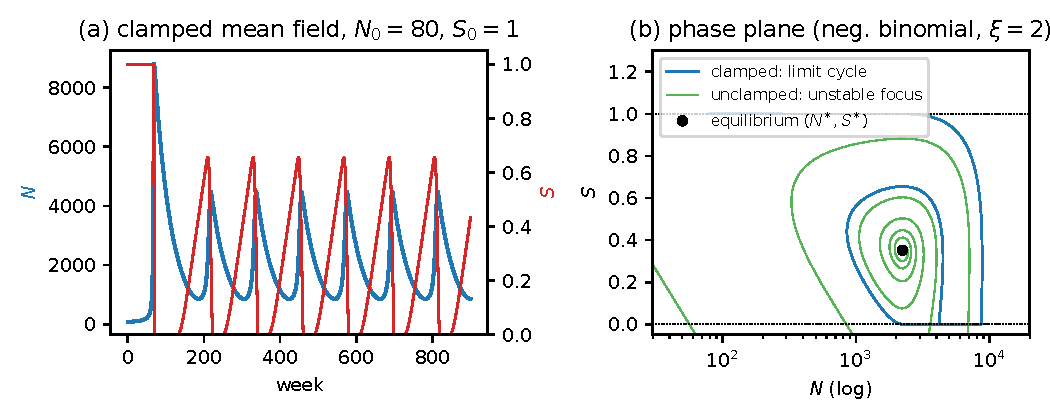
\includegraphics[width=\textwidth]{fig_mf_ode.pdf}
\caption{Two-variable mean field~\eqref{eq:mf2} with negative-binomial occupancy ($\xi=2$). (a)~$N(t)$ and $S(t)$
from $N_0=80$ and $S_0=1$: one overshoot followed by
a periodic limit cycle. (b)~Phase plane: the clamped system (blue) converges to the maximal orbit; without clamping
(green) the equilibrium is an unstable focus whose amplitude grows until it hits $S=0$ or $S=1$.}
\label{fig:ode}
\end{figure}

\paragraph{Homogeneous collapse versus healthy pockets.}
The two-variable model lacks demographic inertia. An age-structured mean field and a well-mixed variant of the
agent-based model (Poisson occupancy) both predict a single hump followed by deterministic extinction
(Fig.~\ref{fig:mfabm}): at the peak the whole young cohort reaches $s\approx0$ at once, recovering to viability
$s_v=R_0^{-1/3}\approx0.31$ takes $s_v/r\approx30$ weeks, and by then the cohort has left its fertile window. The
well-mixed agent-based model gives $N_{\max}=8860\pm80$, $t_{\rm ext}=160\pm12$ weeks and 40/40 extinctions; the
age-structured mean field gives $t_{\rm ext}=203$ weeks.
The oscillations of the spatial model are produced instead by heterogeneity. A minority of individuals living in
uncrowded cells, which we call \emph{healthy pockets} (10--20\% with $s>0.2$ at the peak), keeps $s\approx1$ and
repopulates the trough. Their effective fecundity exceeds $S^3$ by a factor 10--20 at the peak, so the first-moment
closure fails exactly where it matters. In the age-structured mean field a fixed fraction $\rho$ of pocket
individuals turns extinction into sustained oscillations above a sharp threshold $\rho_c\approx2.2\%$ (Poisson
occupancy) to $2.9\%$ ($\xi=2$), at which the trough equals the Allee threshold, $N_{\min}\approx N_A$. That
threshold assumes that pocket individuals experience no crowding at all ($f_P=0$), whereas the pockets of the
agent-based model are only less crowded, so the comparison is qualitative. The three regimes found when scanning
the aggregation strength $\alpha$ in the core model without rules are: (I)~homogeneous overshoot for small $\alpha$ with long-lived
mixing; (II)~a source--sink coexistence sustained by healthy pockets; (III)~collapse by aggregation, when clusters
exceed $m_c$ at low $N$ and no healthy pocket survives. Healthy pockets are an emergent property of the core model and
are unrelated to the refuges of rule R7.

\begin{figure}[ht]
\centering
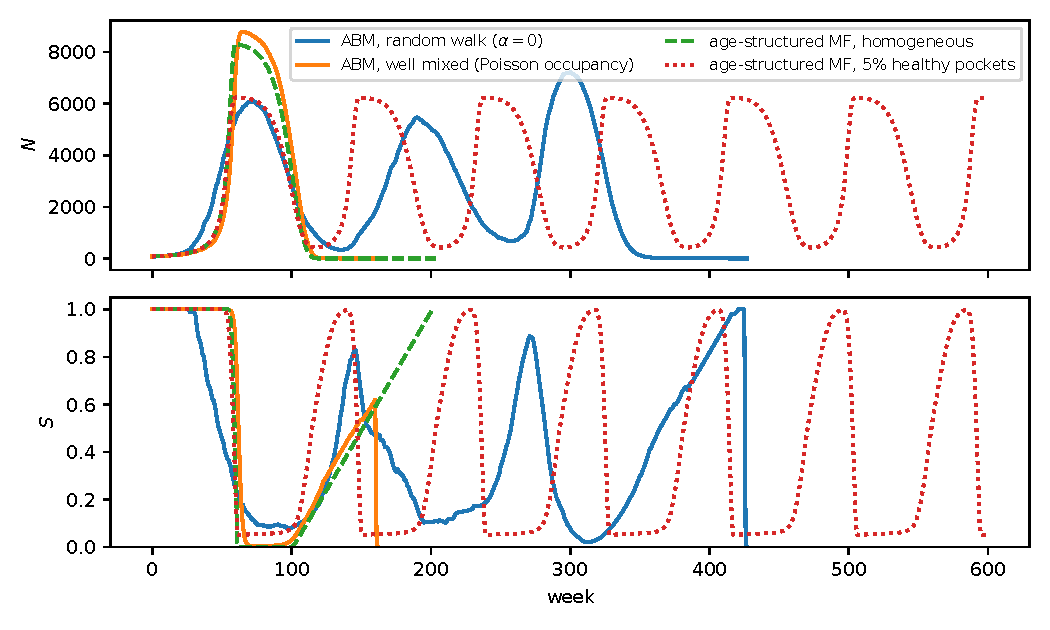
\includegraphics[width=\textwidth]{fig_mf_vs_abm.pdf}
\caption{Population and mean social state for the spatial agent-based model with random motion, the well-mixed
agent-based model (Poisson occupancy), the homogeneous age-structured mean field and the same mean field with a 5\%
fraction of healthy-pocket individuals. Homogeneous descriptions collapse once; healthy pockets produce the
oscillatory regime.}
\label{fig:mfabm}
\end{figure}

\paragraph{Extinction and the absence of secular drift.}
Because the attractor is a cycle, extinction occurs at the troughs, when $N_{\min}$ falls below the Allee threshold
of an aged population. The short-lived control is bimodal. In the exploratory ensemble ($\alpha=1.4$, $n=100$), 49\% [39, 59] of
the colonies die in the first collapse ($t\le184$ weeks), and the survivors have a hazard of $7\times10^{-5}$ per
week [$2.6$, $15$]$\times10^{-5}$ (Fig.~\ref{fig:kmdrift}a); a piecewise-constant hazard is strongly preferred to a
constant one (likelihood ratio 148, $p<10^{-16}$), while the tail alone is compatible with an exponential (Weibull
shape 0.67, $p=0.28$). The independent production ensemble ($n=100$, $T=1000$) gives an early fraction
of 0.44 [0.35, 0.54] with the split at 1.5 times the median event time, 0.42--0.45 for splits between 1.25 and 2.5
times the median, and a tail hazard of $(0.5$--$1.1)\times10^{-4}$ per week; 53 of 100 colonies were still alive at
$T$. Extinction is a mixture of a deterministic-like early mode and a rare late mode, not a heavy-tailed law.
The inheritance rule $s_{\rm pup}=s_{\rm mother}$ was conjectured to produce a secular downward drift of successive
peaks. The mean field says otherwise: mothers are weighted by $s_f^2s_m$ in the birth flux, so newborns carry
$\bar s_{\rm birth}=\mathbb E[s^3]/\mathbb E[s^2]\ge S$; inheritance acts as \emph{selection}, and the clamp at $S=1$
erases memory in every deep trough. The slope of $\log N_{\rm peak}$ per cycle (first peak excluded) is
$+0.027\pm0.019$ for $\alpha=0$ (40 runs, 2000 weeks) and $+0.005$ [$-0.001$, $+0.012$] for $\alpha=1.4$ (50 runs
with at least four peaks; within-run regression $+0.001\pm0.002$); no run shows a significant negative
Mann--Kendall trend (Fig.~\ref{fig:kmdrift}c), and the preregistered production ensemble gave $+0.007$ [$-0.014$,
$+0.027$] (Wilcoxon $p=0.41$). Collapse in the short-lived control is thus \emph{contingent}: it requires the recovery number
$\Pi_R=r\,\tau_{\rm disp}/s_v$ ($\tau_{\rm disp}$ the fertile time left after crowding) to be below one and the
fraction of healthy pockets to be below $\rho_c$.

\begin{figure}[ht]
\centering
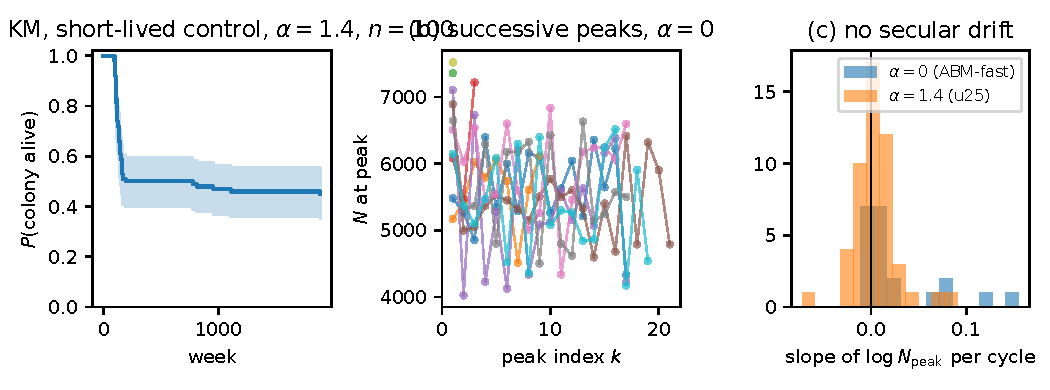
\includegraphics[width=\textwidth]{fig_km_drift.pdf}
\caption{(a)~Kaplan--Meier survival of the colony for the short-lived control ($\alpha=1.4$, 100 replicates, right-censored at
2000 weeks) with Greenwood band. (b)~Successive peak populations for ten runs with $\alpha=0$. (c)~Per-run slope of
$\log N_{\rm peak}$ versus cycle index: no secular drift.}
\label{fig:kmdrift}
\end{figure}

\paragraph{Demography and local occupancy.}
Let $\nu=N/|G|$ be the mean number of mice per cell ($|G|=900$). With the parameters of the short-lived control the logistic hazard
gives a life expectancy of 44.8 weeks, with death almost deterministically ``of old age''. A female that always
finds a mate and keeps $s=1$ produces $R_0=\tfrac12\,p_0\bar L q_0\,\tau_{\rm fert}\approx35$ daughters over her
reproductive window (70 with the long-lived demography of the candidates), so reproduction is limited by
\emph{mate encounter}, not by fecundity: a reproductive female conceives only if a reproductive male shares her
cell. Under random mixing the per-capita birth rate
\begin{equation}
 b(N)=\phi_F\,p_0\bar L q_0\,\bigl(1-e^{-\phi_M N/|G|}\bigr)
 \label{eq:allee}
\end{equation}
increases with $N$: the model has a built-in \emph{Allee effect}, with a deterministic extinction threshold
$N_A\approx61$ for $s\equiv1$. Here $\phi_M\approx\phi_F\approx0.42$ are the fractions of reproductive males and
females in the stationary age distribution; during growth the age structure is younger, so
Eq.~\eqref{eq:allee} is an approximation there. The latency of small founding groups and the failure of very small
ones follow from~\eqref{eq:allee}.
Social deterioration is driven by the local excess occupancy $(m_i-m_c)_+$. With independent positions the expected
weekly loss is $\gamma D(\nu)$, $D(\nu)=\mathbb E[(1+X-m_c)_+]$ with $X\sim\mathrm{Poisson}(\nu)$. Being a Poisson
tail expectation, $D$ is extremely convex ($D=0.0014$ at $\nu=2$, $0.10$ at $\nu^*=4.13$, $1.04$ at $\nu=7$), so
the social state behaves as a \emph{switch}: in the core model ($r/\gamma=0.1$) recovery dominates up to
$N^*=|G|\nu^*\approx3700$, and deterioration of order one per week sets in just above it. Pups are born in their
mother's cell, so the occupancy is clustered (index of dispersion 3--6 during growth for $\alpha=0$, up to 29 at the
peak for $\alpha=1.4$). A negative-binomial occupancy with dispersion $\xi$ captures this and lowers $N^*$ to 2200
for $\xi=2$; affinity-driven motion lowers $\xi$ further, which is why the peak decreases monotonically with
$\alpha$.

\paragraph{Irreversibility: rules R1 and R2.}
In the core model, recovery is an individual process that only needs time: an adult with $s_0\approx0$ returns to
$s_v$ in $(s_v-s_0)/r$ weeks, within its fertile window. Under R1 an adult is a ratchet ($\dot s\le0$), and recovery
becomes a \emph{lineage} process: only pups gain, and producing a pup requires reproduction, whose fecundity scales
as $s_f^2s_m$. Table~\ref{tab:lineage} gives the expected number of descendants that a lineage accumulates before
it reaches viability. It is the expected value of a branching process without learning from neighbours outside the
lineage, so it is a heuristic bound, not a prediction. With the long-lived demography of the candidates
($R_0\approx70$, $s_v=R_0^{-1/3}\approx0.24$) the expected number is at most $10^{-2}$ for $s_0\le0.05$, whatever the
gain per generation and the partner. It is 0.01--0.07 for $s_0=0.1$ when the partner is equally deteriorated, and up
to 0.7 when the partner is healthy, because fecundity then scales as $s^2$ in the first generation. A lineage of
$s_0\approx0.2$ can recover. The bottleneck at small $s_0$ is the fecundity of deteriorated parents, not the gain
per generation. In addition, every crowding hit on a healthy adult is permanent, so healthy pockets erode instead of
regenerating. The transplants of Section~\ref{sec:res-Q} confirm the bottleneck (animals with $s\approx0$ never
found a colony; animals with $s\approx0.36$ found one in 8\% of the trials under R1 against 95\% without it) but not
the second part of the argument: the offspring of intermediate founders settle at their parents' level instead of
collapsing.
Under R2 recovery is $r[(1-\lambda)+\lambda\bar s_V]$, with $\bar s_V$ the mean state of the neighbours. In the
homogeneous limit $S=0$ is absorbing for $\lambda=1$, and for $\lambda<1$
\begin{equation}
 T_{\rm rec}(\lambda)=\frac{1}{r\lambda}\,
 \ln\frac{(1-\lambda)+\lambda s_v}{(1-\lambda)+\lambda S_0},
 \label{eq:trec}
\end{equation}
so the colony is irreversible when $T_{\rm rec}$ exceeds the fertile time left after crowding. Unlike R1, R2 depends
on $r$, and in the spatial model a healthy cell is a focus from which $s$ spreads, so \eqref{eq:trec} gives lower
bounds for the threshold. A kinetic mean field with persistent cell disorder (Appendix~\ref{app:kin},
Table~\ref{tab:thr}, Fig.~\ref{fig:thr}) quantifies both rules for $r\in\{0.01,0.03\}$, the only rates it was run
with, and 10 seeds per cell (10 extinctions out of 10 have a Wilson interval of $[0.72,1]$): with the long-lived
demography, R1 gave extinction in 10/10 seeds for every $a_w\le24$ weeks at both rates, so within this range its
effect does not depend on $r$, and the agent-based plane $(r,a_w)$ later extended this to $r\in[0.02,0.3]$; R2 alone
extinguishes the long-lived colony when $\lambda$ exceeds a threshold that grows with $r$; the threshold
$\lambda_c$ is defined throughout as the first value of the grid $\{0,0.3,0.5,0.7,0.9,1\}$ at which at least half of
the 10 seeds go extinct, so it is $\lambda_c\le0.3$ at $r=0.01$ (8/10 seeds at $\lambda=0.3$; 10/10 from 0.5 on),
$\lambda_c\in(0.7,0.9]$ at $r=0.03$, and $\lambda_c\in(0.5,0.7]$ at $r=0.03$ with faster mixing; with the short
life span R2 needs $\lambda\ge0.9$ and fast mixing, and even then extinction is not certain (at most 8/10 seeds).

\paragraph{Thresholds of R1 and R2 in the kinetic mean field.}
In the kinetic mean field (Appendix~\ref{app:kin}), calibrated to the quasi-stationary regime of the short-lived control, R1
alone with the short life span and persistent healthy pockets reduces the rebound but does not extinguish the
colony ($P_{\rm ext}\le0.3$); faster mixing makes it lethal for $a_w\le12$, with weak dependence on $r$. In the
long-lived scenario ($a_{\max}=120$, fertility to 80 weeks) R1 gives $P_{\rm ext}=1$ and zero rebound for
$a_w\le24$ at both $r=0.01$ and $0.03$ (10/10 seeds per cell, Wilson interval $[0.72,1]$), with the critical window
$a_w^c\in(24,48)$ at $r=0.03$ and above 48 weeks at $r=0.01$ (same definition: first grid value with at least half
of the seeds extinct). R2 requires $\lambda\gtrsim0.9$ with the short life span, and in the long-lived scenario
$\lambda_c\le0.3$ ($r=0.01$; $P_{\rm ext}=0.8$ already at $\lambda=0.3$) or $\lambda_c\in(0.7,0.9]$ ($r=0.03$), in
agreement with Eq.~\eqref{eq:trec}; with faster mixing $\lambda_c\in(0.5,0.7]$ at $r=0.03$ (Fig.~\ref{fig:thr}). For
$\lambda=1$, Eq.~\eqref{eq:trec} gives $T_{\rm rec}=\ln(s_v/S_0)/r=274$--413 weeks for the measured
$S_{\min}\approx0.01$--0.02 and $r=0.01$.

\begin{figure}[ht]
\centering
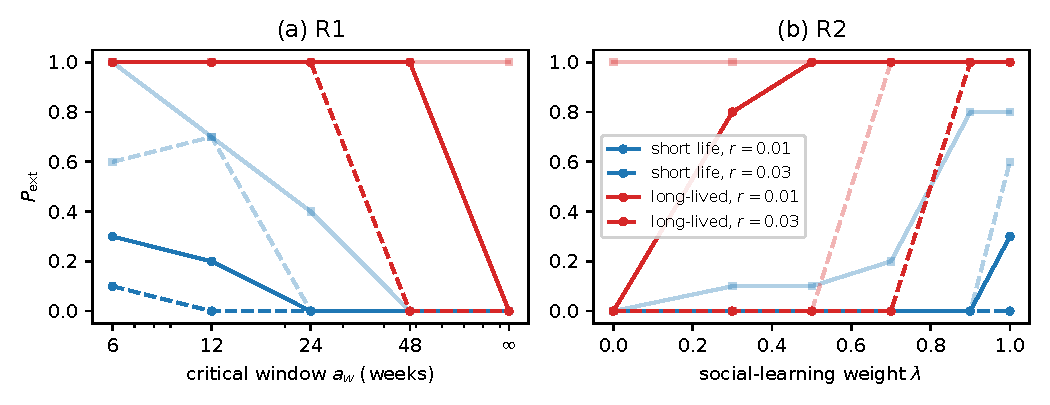
\includegraphics[width=\textwidth]{fig_thresholds.pdf}
\caption{Extinction probability in the kinetic mean field (10 seeds, 1500 weeks) as a function of (a)~the critical
window $a_w$ of R1 and (b)~the social-learning weight $\lambda$ of R2, for the short ($a_{\max}=60$) and long ($a_{\max}=120$) life spans
and two recovery rates. Circles: persistent healthy pockets ($\xi_c=0.5$, $\tau_F=8$); faint squares: faster mixing
($\xi_c=1$, $\tau_F=5$).}
\label{fig:thr}
\end{figure}

\paragraph{Status of the exploratory mean-field statements.}
\begin{itemize}
  \item The kinetic mean field predicted that R1 with the long-lived demography gives $P_{\rm ext}=1$ and no rebound
    for every window $a_w\le24$ at the two rates it was run with ($r=0.01$ and $0.03$). The agent-based plane
    $(r,a_w)$ extends this to $r\in[0.02,0.3]$: $P_{\rm ext}=1$ at 48 of 48 points. Without the window, extinction
    occurs only for $r\le0.03$, and recurrent growth (A2) dominates for $r\ge0.07$ (Appendix~\ref{sec:res-planes}).
  \item That R1 blocks the recovery of transplanted adults is confirmed. That R2 with $\lambda=1$ alone blocks it is
    not: without R1, phase-D transplants recover in 0/60 trials at week 86 but in 10/60 at week 126, and animals of
    intermediate state found colonies in 50/60 trials (Appendix~\ref{sec:res-transplant}), as Eq.~\eqref{eq:trec}
    allows for $r=0.1$ ($T_{\rm rec}\approx27$ weeks).
  \item The ageing decline, $(T_{\rm ext}-t_{\rm pk})/t_{\rm pk}\approx2$ with a small spread, is confirmed (2.07
    with $t_{\rm pk}=\arg\max N$), but the ratio depends on how the peak time is defined on the plateau
    (Appendix~\ref{app:res-production}).
  \item Not tested in the production sweeps: the thresholds in $\lambda$ ($\lambda=1$ in all candidates), the effect
    of long-range mixing (the jump rule was discarded) and critical slowing down (the candidates do not oscillate).
\end{itemize}

\subsection{Production ensembles: details}
\label{app:res-production}

Table~\ref{tab:res-production-si} completes Table~\ref{tab:res-production} with the desirable patterns, the timings
of the boom and further magnitudes.

\begin{table}[ht]
\centering
\caption{Production ensembles in full (same ensembles and precision as Table~\ref{tab:res-production}): essential
patterns, transplants (founding transplants over trials, 60 replicates per arm; O12b pools both sexes; phase D at
$1.75\,t'_{\rm pk}$ of each colony, and the third row at week 95 in every arm), anti-patterns, magnitudes, desirable
patterns (fraction of passing runs), timings (medians over runs) and further magnitudes. ``PASS or MARGINAL'' for
O13b counts the runs in which the evaluator finds the isolated class later-born at least marginally.}
\label{tab:res-production-si}
\scriptsize
\setlength{\tabcolsep}{3pt}
\begin{tabular}{@{}llccccccc@{}}
\toprule
ID & Pattern & \textsf{C1} & \textsf{C1}$'$ & \textsf{C0} & $\alpha{=}0$ & \textsf{C2} & short-lived & long-lived \\
\midrule
O4 & peak below capacity, free space & 1.00 & 1.00 & 1.00 & 0.00 & 0.90 & 0.87 & 0.08 \\
O5 & natality ends at high $N$ & 0.99 & 0.85 & 1.00 & 1.00 & 0.81 & 0.25 & 0.90 \\
O6 & no rebound & 1.00 & 1.00 & 1.00 & 1.00 & 0.98 & 0.45 & 0.97 \\
O7 & extinction & 1.00 & 0.99 & 1.00 & 1.00 & 0.98 & 0.47 & 0.98 \\
O10 & adult deterioration before peak & 1.00 & 1.00 & 1.00 & 1.00 & 1.00 & 1.00 & 1.00 \\
O11 & late cohorts fail & 1.00 & 0.97 & 1.00 & 1.00 & 0.99 & 0.00 & 0.00 \\
O13 & two deteriorated classes & 1.00 & 1.00 & 0.92 & 1.00 & 1.00 & 0.00 & 0.00 \\
O13p & \quad persistent isolated class & 1.00 & 1.00 & 0.00 & 0.00 & 0.94 & 0.00 & 0.00 \\
O17 & Calhoun-like run (O17) & 0.99 & 0.83 & 0.92 & 0.00 & 0.72 & 0.00 & 0.00 \\
\midrule
O17p & \textbf{primary outcome} & 0.99 & 0.83 & 0.00 & 0.00 & 0.70 & 0.00 & 0.00 \\
 & \quad 95\% Wilson interval & 0.97--1.00 & 0.78--0.88 & 0.00--0.02 & 0.00--0.02 & 0.64--0.76 & 0.00--0.04 & 0.00--0.04 \\
\midrule
O12 & transplants found: phase B & 52/60 & 46/60 & 47/60 & -- & 49/60 & -- & -- \\
 & \quad phase D ($1.75\,t'_{\rm pk}$) & 0/60 & 0/60 & 0/60 & -- & 0/60 & -- & -- \\
 & \quad week 95, all arms & 0/60 & 0/60 & 0/60 & -- & 0/60 & -- & -- \\
O12b$^\dagger$ & \quad D + healthy partners & 0/120 & 0/120 & 0/120 & -- & 2/120 & -- & -- \\
A1--A4 & anti-patterns triggered & none & none & none & none & A2: 0.02 & A2: 0.55 & A2: 0.03 \\
\midrule
& $\rho_{\rm pk}=N_{\rm pk}/K_\gamma$ & 0.36 & 0.33 & 0.42 & 0.71 & 0.42 & 0.77 & 0.85 \\
& empty cells at peak, $f_0$ & 0.16 & 0.52 & 0.19 & 0.03 & 0.11 & 0.30 & 0.59 \\
& persistent isolated, $\Phi^{\rm pers}_{\rm BO}$ & 0.17 & 0.16 & 0.01 & 0.09 & 0.13 & 0.00 & 0.00 \\
& median $T_{\rm ext}$ (weeks, KM) & 169 & 182 & 166 & 155 & 218 & -- & 186 \\
& spread of $T_{\rm ext}$ (KM IQR/median) & 0.09 & 0.12 & 0.08 & 0.05 & 0.14 & -- & 0.16 \\
\midrule

O8 & senescent decline & 0.62 & 0.21 & 0.82 & 0.97 & 0.00 & 0.09 & 0.37 \\
O8b & slow initial decline & 1.00 & 1.00 & 1.00 & 1.00 & 1.00 & 1.00 & 1.00 \\
O9 & old, female-biased remnant & 0.45 & 0.29 & 0.44 & 0.49 & 0.30 & 0.21 & 0.37 \\
O10b & functional growth phase & 0.02 & 0.01 & 0.18 & 1.00 & 0.00 & 1.00 & 0.19 \\
O11b & few late-born females conceive & 1.00 & 1.00 & 1.00 & 1.00 & 1.00 & 1.00 & 0.97 \\
O13b & isolated class later-born & 0.00 & 0.00 & 0.00 & 0.00 & 0.00 & 0.00 & 0.00 \\
O14 & aggregation with free space & 1.00 & 1.00 & 1.00 & 0.00 & 1.00 & 1.00 & 1.00 \\
O15 & infant mortality $\to$ 1 & 0.01 & 0.00 & 0.00 & 0.01 & 0.01 & 0.00 & 0.01 \\
O15b & conceptions without viable young & 0.57 & 0.70 & 0.46 & 0.28 & 0.45 & 0.15 & 0.09 \\
O13b & \quad PASS or MARGINAL & 0.01 & 0.04 & 0.04 & 0.00 & 1.00 & 0.16 & 0.63 \\
\midrule
& $t'_{\rm pk}$ (weeks, median) & 34 & 35 & 33 & 31 & 62 & 31 & 45 \\
& $t_{\rm pk}=\arg\max N$ (median) & 55 & 61 & 53 & 44 & 80 & 35 & 66 \\
& plateau length (median) & 51 & 50 & 54 & 59 & 28 & 9 & 45 \\
& $t_{B99}$ (median) & 40 & 44 & 38 & 33 & 86 & 980 & 55 \\
& \quad 95\% CI of the KM median & 167--171 & 180--185 & 165--167 & 154--156 & 217--222 & -- & 181--190 \\
& $P_{\rm ext}(T)$ & 1.00 & 0.99 & 1.00 & 1.00 & 0.98 & 0.47 & 0.98 \\
& CV of $T_{\rm ext}$ (extinct runs) & 0.07 & 0.16 & 0.07 & 0.06 & 0.12 & 0.45 & 0.20 \\
& $(T_{\rm ext}-t_{\rm pk})/t_{\rm pk}$ (extinct) & 2.13 & 2.15 & 2.16 & 2.60 & 1.88 & 2.78 & 2.02 \\
\bottomrule

\end{tabular}
\end{table}

\paragraph{The plateau and the definition of the peak time.}
In the 200 runs of \textsf{C1} (medians, with interquartile ranges in brackets), the population first comes within
2\% of its maximum at week 34 [32, 36] and leaves that band at week 86 [85, 86], so the plateau lasts 51 [49, 53]
weeks. The maximum itself, $t_{\rm pk}=\arg\max N$, is reached at week 55 [50, 60], 21 [16, 25] weeks after the
plateau begins, and coincides with the last surviving birth in 69\% of the runs. The 99th percentile of the births
falls at $1.17\,t'_{\rm pk}$ [1.12, 1.24], and the decline ratio is $(T_{\rm ext}-t'_{\rm pk})/t'_{\rm pk}=3.97$
[3.72, 4.29] against 2.07 [1.85, 2.33] with $t_{\rm pk}$. The primary evaluator uses $t'_{\rm pk}$ and
$t_{B99}$; Appendix~\ref{app:res-rescoring} gives every pattern with both definitions.

\paragraph{The escaped run.}
One \textsf{C1}$'$ run in 200 was still alive at $T=600$: it fails O7 and is censored in the survival analysis. No
\textsf{C1} run escaped in the reference ensemble; in the ensemble at $T=700$ all 200 died.

\subsection{Survival of colonies}
\label{sec:res-survival}

Fig.~\ref{fig:res-survival} shows Kaplan--Meier estimates of colony survival; runs still alive at the horizon enter
as right-censored observations.
\begin{itemize}
  \item \textsf{C1} and \textsf{C0} die out within a narrow window. Their median extinction times are 169
    [167, 171] and 166 [165, 167] weeks, and the Weibull shapes of the collapse are 14.7 and 11.9.
  \item \textsf{C1}$'$ dies at 182 [180, 185] weeks, with a longer tail (Weibull shape 3.3 without a cure fraction,
    4.4 with $\hat\pi=0.005$, the single censored colony).
  \item \textsf{C2} dies later, at 218 [217, 222] weeks, and with more spread (KM interquartile range over median
    0.14). Four of its 200 colonies persist to $T=700$ and recovered natality (A2).
  \item The short-lived control is a mixture: 47 of 100 colonies died by $T=1000$, 44\% [35, 54] in the first
    collapse, the others in a quasi-stationary oscillation with a tail hazard of $0.7\times10^{-4}$ per week
    (Weibull shape 0.60 over all times; cure fraction $\hat\pi=0.53$).
  \item In the long-lived control 98 of 100 colonies die, at 186 [181, 190] weeks; with the
    initial condition of \textsf{C1} (null-model ensemble, $n=200$), 199 of 200 die, with a KM spread of 0.160.
\end{itemize}
The survival curves of \textsf{C1} and the short-lived control differ (log-rank $\chi^2=53$, $p=3\times10^{-13}$). A likelihood-ratio
test of the cure fraction is degenerate for \textsf{C1} (no censored colony) and is not reported; because no
\textsf{C1} colony dies before about 140 weeks, a Weibull without a location parameter mixes location and shape, so
the shape 14.7 should not be read as a hazard exponent. The Kaplan--Meier quantiles are the safer summary.
Among the single ablations, removing R1 is the only one that changes survival qualitatively (27 of 120 colonies go
extinct by week 600); removing AV delays extinction by about 18 weeks (median 185 against 167); removing R2 or R7
leaves the survival curve unchanged (170 and 167).

\begin{figure}[ht]
  \centering
  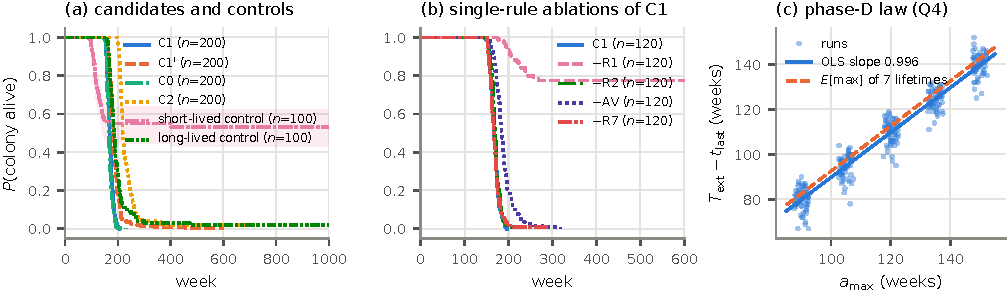
\includegraphics[width=\textwidth]{fig_res_survival.pdf}
  \caption{Survival of colonies.
  \textbf{(a)}~Kaplan--Meier curves of the candidates and of the short-lived and long-lived controls (reference ensemble for
  \textsf{C1}, \textsf{C1}$'$ and \textsf{C0}). Shaded bands are log--log Greenwood intervals for \textsf{C1} and the
  short-lived control. Censoring is at $T=600$ (\textsf{C1}, \textsf{C1}$'$, \textsf{C0}), $T=700$ (\textsf{C2}) and
  $T=1000$ (short-lived and long-lived controls).
  \textbf{(b)}~Single-rule ablations of \textsf{C1} ($n=120$, $T=600$).
  \textbf{(c)}~Phase-D law (Q4): time from the last birth to extinction against $a_{\max}$ ($n=300$, jittered). The
  solid line is the OLS fit. The dashed line is the expected maximum of $n_{\rm last}$ logistic lifetimes, with
  $n_{\rm last}=7$, the median number of births in the last ten weeks.}
  \label{fig:res-survival}
\end{figure}

\subsection{Ablations: factorial model and the minimal candidate}
\label{app:res-ablations}

A Firth logistic model of the full $2^4$ factorial (exploratory, Benjamini--Hochberg at 10\%) gives, on the logit
scale: positive main effects for R7 and R2 ($4.9\pm1.2$ each), none for R1 ($-0.5\pm1.1$, $p=0.63$) or AV
($-0.5\pm1.1$, $p=0.68$), positive interactions R1:R7 and R1:R2 ($6.6\pm1.9$) and weaker ones R2:AV and AV:R7
($3.9\pm1.8$, $p=0.036$). R1 acts only together with R2 or R7, because without them O17p is zero whether R1 is present
or not. Unlike in \textsf{C0} (Section~\ref{sec:calib-ablations}), stronger attraction does not rescue the ablation
of R1: with $\alpha=6$, O17p is 0.04.
Table~\ref{tab:res-c1p} compares \textsf{C1}$'$ with \textsf{C1} in the reference ensemble and in the factorial, and
gives its single ablations (the double ablations of \textsf{C1} that remove AV, $n=40$).

\begin{figure}[ht]
  \centering
  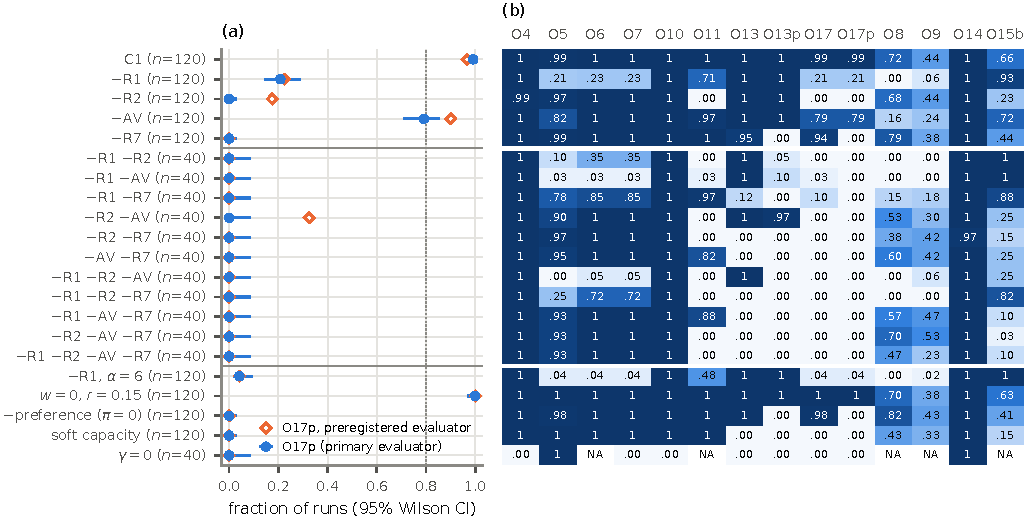
\includegraphics[width=\textwidth]{fig_res_ablations.pdf}
  \caption{Ablations of \textsf{C1}.
  \textbf{(a)}~Primary outcome O17p with the primary evaluator (filled, 95\% Wilson interval) and with the preregistered
  evaluator (open diamonds). Rows are \textsf{C1} and its single ablations ($n=120$), double to quadruple ablations
  ($n=40$), and implementation variants. The dotted line marks the 0.8 threshold for an essential pattern.
  \textbf{(b)}~Fraction of passing runs for each pattern (primary evaluator). NA marks a pattern that is not
  applicable in any run; with $\gamma=0$ the colonies never go extinct.}
  \label{fig:res-ablations}
\end{figure}

\begin{table}[ht]
  \centering
  \caption{The minimal candidate \textsf{C1}$'$ (= \textsf{C1} without AV). Top: reference ensemble ($n=200$,
  $T=600$); $p$ is the two-sided Fisher test against \textsf{C1}. Middle: the AV arm of the preregistered factorial
  ($n=120$); $p$ is the one-sided test of Q2 before Holm adjustment. Bottom: single ablations of \textsf{C1}$'$
  ($n=40$); $p$ is the one-sided Fisher test against the \textsf{C1}$-$AV arm of the factorial. O17p with 95\% Wilson
  interval; other columns are fractions of passing runs, and $f_0$ is the mean fraction of empty cells at the peak.}
  \label{tab:res-c1p}
  \small
  \begin{tabular}{@{}lrrlllllll@{}}
    \toprule
    Arm & $n$ & $T$ & O17p & $p$ & O5 & O11 & O13p & O8 & $f_0$ \\
    \midrule
    C1 & 200 & 600 & 0.99 [0.97, 1.00] &  & 0.99 & 1.00 & 1.00 & 0.62 & 0.16 \\
C1$'$ $=$ C1 $-$ AV & 200 & 600 & 0.83 [0.78, 0.88] & $1.0\times10^{-9}$ & 0.85 & 0.97 & 1.00 & 0.21 & 0.52 \\
\midrule
C1 (factorial) & 120 & 600 & 0.99 [0.95, 1.00] &  & 0.99 & 1.00 & 1.00 & 0.72 & 0.16 \\
C1 $-$ AV (factorial) & 120 & 600 & 0.79 [0.71, 0.85] & $1.1\times10^{-7}$ & 0.82 & 0.97 & 1.00 & 0.16 & 0.52 \\
\midrule
C1$'$ $-$ R1 & 40 & 600 & 0.00 [0.00, 0.09] & $<10^{-16}$ & 0.03 & 0.03 & 0.10 & 0.00 & 0.50 \\
C1$'$ $-$ R2 & 40 & 600 & 0.00 [0.00, 0.09] & $<10^{-16}$ & 0.90 & 0.00 & 0.97 & 0.53 & 0.51 \\
C1$'$ $-$ R7 & 40 & 600 & 0.00 [0.00, 0.09] & $<10^{-16}$ & 0.95 & 0.82 & 0.00 & 0.60 & 0.76 \\
\bottomrule

  \end{tabular}
\end{table}

\subsection{Confirmatory tests: further details and the preregistered evaluator}
\label{app:res-Q}

Table~\ref{tab:res-Qcmp} gives the confirmatory family with the primary evaluator and with the preregistered evaluator;
the latter replicates the preregistered analysis on the production runs.
\begin{itemize}
  \item \emph{Q1.} The transplanted \textsf{C1} animals are 37--64 weeks old at $1.75\,t'_{\rm pk}$ (week 60), 59--80
    at $1.75\,t_{\rm pk}$ (week 97) and 65--80 at week 95; the fertile window closes at 80 weeks. In arm $X$ the
    founding rates are 51/60, 12/60 and 5/60 (McNemar $p=4\times10^{-16}$, $2\times10^{-4}$ and $0.03$).
  \item \emph{Q4.} The law explains why O8 depends on longevity: O8 passes in 0.15, 0.30, 0.67, 0.83 and 0.92 of the
    runs for $a_{\max}=90$, 105, 120, 135 and 150, while every essential pattern is unchanged (O17p 0.93--1.00).
  \item \emph{Q5.} O13 fails only for the strongest aversion with the strongest attraction ($\kappa=0.3$, $\alpha=8$;
    $n^*\approx3.2$), where the crowded fraction falls to the 10\% threshold. The one-sided test of $b_2<0$ gives
    $p=1$ (Pearson $\phi=1.0$).
  \item \emph{Q6.} Profile-likelihood intervals: $[-0.15,-0.10]$ binomial and $[-0.20,-0.05]$ quasi-binomial
    ($\phi=3.1$) with the primary evaluator; $[0.20,0.40]$ and $[0.15,0.50]$ ($\phi=1.8$) with the preregistered
    evaluator. The grid of the profile is $\theta\in[-1,3]$ in steps of 0.05. The quasi-binomial $p$ is the one that
    enters the Holm sequence. The additive model in standardised $\log r$ and $\log a_w$ with quadratic terms beats
    the single-index model by $\Delta{\rm QAIC}=27.8$ over the 48 points and by 27.7 without the point that fails
    through the persistent class (dispersion of the additive model 1.9). With the preregistered evaluator the comparison
    goes the other way: the single-index model is preferred by $\Delta{\rm QAIC}=11$, so the change of criterion
    changes the adequate model as well as the sign of $\hat\theta$. With the primary evaluator the O17p boundary of
    the plane is nearly vertical in $r$ (at least 0.67 for $r\le0.10$ and at most 0.60 for $r\ge0.2$ at every
    window), which is why the prediction is reported as ``not supported'' rather than as a reversal.
  \item \emph{Q7.} The logistic fit of the preregistered plane places the extinction boundary at $\gamma=0$ at
    $w+0.24\,\Lambda=0.215$, that is $\hat\sigma=4.65$ and $\hat\varphi=1.11$ in the form $\sigma w+\varphi\Lambda=1$
    (Fig.~\ref{fig:res-planes-social}b). The grid brackets the boundary coarsely: at $w=0$ colonies go extinct for
    $r\le0.05$ (0.9 at $r=0.07$) and survive for $r\ge0.10$; at $w=0.1$ the change happens between $r=0.03$ and 0.05;
    at $w\ge0.2$ no colony goes extinct. In the subcritical corner the median peak is 6\,500--11\,500 individuals at
    weeks 77--96 ($\rho_{\rm pk}$ between 0.85 and 1.66 over the 120 runs), and O4 fails in every run.
\end{itemize}

\begin{table}[ht]
  \centering
  \caption{The confirmatory family with the primary evaluator (left) and with the preregistered evaluator (right), on
  the same runs. Holm correction over seven tests within each column set; the $p$ of Q6 is quasi-binomial. The
  preregistered evaluator takes the transplant of Q1 at $1.75\,t_{\rm pk}$ with $t_{\rm pk}=\arg\max N$, as
  preregistered.}
  \label{tab:res-Qcmp}
  \scriptsize
  \resizebox{\textwidth}{!}{%
  \begin{tabular}{@{}lp{5.2cm}lccp{5.2cm}lcc@{}}
    \toprule
    & \multicolumn{4}{c}{primary evaluator} & \multicolumn{4}{c}{preregistered evaluator} \\
    \cmidrule(lr){2-5}\cmidrule(lr){6-9}
    & Estimate & $p_{\rm Holm}$ & Rej. & Met & Estimate & $p_{\rm Holm}$ & Rej. & Met \\
    \midrule
    Q1 & 0/60 vs.\ 51/60 ($P_T=0.85$ [0.74, 0.92]); discordant pairs 51:0 & $1.3\times10^{-15}$ & yes & yes & 0/60 vs.\ 12/60 ($P_T=0.20$ [0.12, 0.32]); discordant pairs 12:0 & $7.3\times10^{-4}$ & yes & no \\
Q2 & 0.99 vs.\ $-$R1 0.21, $-$R2 0.00, $-$AV 0.79, $-$R7 0.00 & $2.2\times10^{-7}$ & yes & no & 0.97 vs.\ $-$R1 0.23, $-$R2 0.17, $-$AV 0.90, $-$R7 0.00 & 0.067 & no & no \\
Q3 & 200/200 vs.\ 47/100; CV 0.066 [0.059, 0.071] & $<10^{-16}$ & yes & yes & 200/200 vs.\ 47/100; CV 0.066 [0.059, 0.071] & $<10^{-16}$ & yes & yes \\
Q4 & slope $0.996\pm0.014$; $\bar r=-2.0\pm0.3$ wk & $<10^{-16}$ & yes & yes & slope $0.996\pm0.014$; $\bar r=-2.0\pm0.3$ wk & $<10^{-16}$ & yes & yes \\
Q5 & $b_2=+185.3\pm64.3$ (convex); no interior maximum & 1.00 & no & no & $b_2=+69.5\pm14.2$ (convex); no interior maximum & 1.00 & no & no \\
Q6 & $\hat\theta=-0.15$ [-0.20, -0.05] (quasi-binomial, $\phi=3.1$) & $<10^{-16}$ & yes & no & $\hat\theta=0.30$ [0.15, 0.50] (quasi-binomial, $\phi=1.8$) & $4.0\times10^{-5}$ & yes & yes \\
Q7 & 120/120 vs.\ 0/30 (30/30 explode) & $<10^{-16}$ & yes & yes & 120/120 vs.\ 0/30 (30/30 explode) & $<10^{-16}$ & yes & yes \\
\bottomrule

  \end{tabular}}
\end{table}

\paragraph{Q7 with the window varied.}
Fig.~\ref{fig:res-q7aw} shows $P_{\rm ext}$ at $\gamma=0$ against $\Lambda=r\,a_w$ for $a_w\in\{6,12,24\}$ and
$w\in\{0,0.05,0.1\}$: six values of $\Lambda$ per window (0.24, 0.36, 0.48, 0.6, 0.84, 1.2; consecutive ratios
1.25--1.5), 54 points, 20 runs each. The analysis fixed before the production runs is a logistic model in $z=\log r+\theta\log a_w$ and $w$,
with a profile-likelihood interval for $\theta$, a likelihood ratio for $\theta=1$ and an equivalence test of the
two exponents (TOST, margin $[2/3,3/2]$). The data do not support that analysis: 51 of the 54 points have
$P_{\rm ext}=0$ or 1 (the other three are 19/20, 14/20 and 5/20), the Pearson dispersion is 0.05 and the maximum
likelihood coefficients diverge, that is, the model is separated. In a separated logistic model the profile
$\ell(\theta)$ is flat wherever $\theta$ keeps the ordering of the points in $z$ that separates zeros from ones and
drops where it breaks it, so the profile interval ($\hat\theta=0.725$ [0.70, 0.75], likelihood ratio 219 for
$\theta=1$) reflects the geometry of the grid rather than sampling error; the fitted
transition widths are $10^{-8}$--$10^{-19}$ in $\log\Lambda$, below the grid spacing at every $a_w$, and the parametric
bootstrap of the fitted boundary ($\hat\sigma=4.3$, $\hat\varphi=1.17$) resamples essentially the same data. None of
these quantities is reported as inference; they are kept, labelled, in \texttt{results\_numbers.json}.
Table~\ref{tab:res-q7aw} gives instead a non-parametric summary per window: the last grid point with
$P_{\rm ext}\ge1/2$ and the first with $P_{\rm ext}<1/2$, which bracket $\Lambda_{1/2}$ to a factor 1.25--1.5; a
log-linear interpolation between them; and, between consecutive windows, the exponent
$\theta_{\rm loc}=1-\log[\Lambda_{1/2}(a_2)/\Lambda_{1/2}(a_1)]/\log(a_2/a_1)$ implied by the brackets (its grid
bounds) and by the interpolated values. At every $w$ the brackets of $a_w=12$ and 24 coincide and that of $a_w=6$ is
one grid step below, so $\theta_{\rm loc}\in(0,1)$ between 6 and 12 weeks (interpolated 0.51, 0.60 and 0.70 for
$w=0$, 0.05 and 0.1) while between 12 and 24 weeks the grid only bounds it within about $(0.5,1.5)$ (interpolated
0.99, 1.00 and 0.88). The equivalence margin $[2/3,3/2]$ is thus resolved in neither interval, and the one firm
statement is qualitative: at a given product $r\,a_w$ a short window with fast learning is less effective than a
long window with slow learning, and a single exponent does not describe the three windows. Resolving $\theta$
would need a grid of ratio about 1.05 around each $\Lambda_{1/2}$ with more runs per point; it was not run.

\begin{figure}[ht]
  \centering
  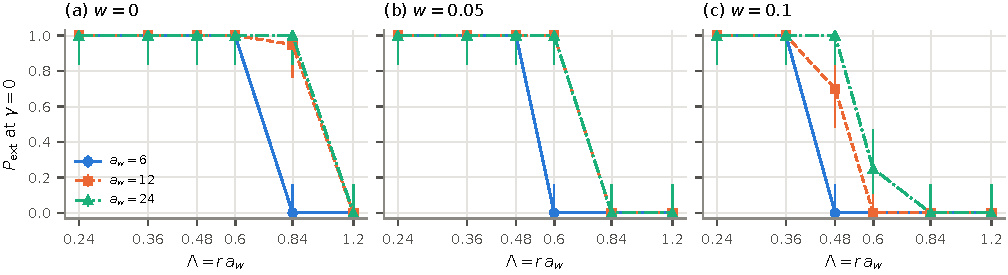
\includegraphics[width=\textwidth]{fig_res_q7aw.pdf}
  \caption{Extinction probability without crowding damage ($\gamma=0$) against $\Lambda=r\,a_w$ for three
  plasticity windows, at three inheritance weights (95\% Wilson intervals, 20 runs per point).}
  \label{fig:res-q7aw}
\end{figure}

\begin{table}[ht]
  \centering
  \caption{Transition of $P_{\rm ext}$ at $\gamma=0$ in $\Lambda=r\,a_w$, by inheritance weight $w$ and window
  $a_w$ (20 runs per point). Columns: the last grid value of $\Lambda$ with $P_{\rm ext}\ge1/2$ and the first with
  $P_{\rm ext}<1/2$, each with its count of extinct runs, which bracket $\Lambda_{1/2}$; its log-linear interpolation;
  and the exponent $\theta_{\rm loc}=1-\log[\Lambda_{1/2}(a')/\Lambda_{1/2}(a_w)]/\log(a'/a_w)$ between this window
  and the next ($a'=12$ for $a_w=6$, $a'=24$ for $a_w=12$): the range allowed by the two brackets, then the value
  from the interpolated $\Lambda_{1/2}$. The preregistered logistic fit is separated (51 of 54 points at
  $P_{\rm ext}\in\{0,1\}$) and is not reported as inference (text).}
  \label{tab:res-q7aw}
  \small
  \begin{tabular}{@{}cclllc@{}}
    \toprule
    $w$ & $a_w$ & last $\Lambda$, $P_{\rm ext}\ge\frac12$ & first $\Lambda$, $P_{\rm ext}<\frac12$ & $\Lambda_{1/2}$ & $\theta_{\rm loc}$ to next window \\
    \midrule
    0 & 6 & 0.6 (20/20) & 0.84 (0/20) & 0.71 & (0.00, 1.00); 0.51 \\
0 & 12 & 0.84 (19/20) & 1.2 (0/20) & 0.99 & (0.49, 1.51); 0.99 \\
0 & 24 & 0.84 (20/20) & 1.2 (0/20) & 1.00 & -- \\
\midrule
0.05 & 6 & 0.48 (20/20) & 0.6 (0/20) & 0.54 & (0.19, 1.00); 0.60 \\
0.05 & 12 & 0.6 (20/20) & 0.84 (0/20) & 0.71 & (0.51, 1.49); 1.00 \\
0.05 & 24 & 0.6 (20/20) & 0.84 (0/20) & 0.71 & -- \\
\midrule
0.1 & 6 & 0.36 (20/20) & 0.48 (0/20) & 0.42 & (0.26, 1.00); 0.70 \\
0.1 & 12 & 0.48 (14/20) & 0.6 (0/20) & 0.51 & (0.68, 1.32); 0.88 \\
0.1 & 24 & 0.48 (20/20) & 0.6 (5/20) & 0.56 & -- \\
\bottomrule

  \end{tabular}
\end{table}

\subsection{Re-scoring with the preregistered evaluator and with each option changed separately}
\label{app:res-rescoring}

Every run of the production program was scored with the primary evaluator, with the full preregistered evaluator and with
each option changed separately: peak time at $\arg\max N$ or at the end of the plateau instead of its start; crowded
class at $m>m_c$ instead of $m>8$; O5 on the last sustained birth instead of $t_{B99}$; the preregistered O4 (no
free-space condition). Table~\ref{tab:res-rescoring} gives O17p for the main arms, and Table~\ref{tab:res-null-v1}
the discriminating power of the redefined criteria with the preregistered evaluator.
\begin{itemize}
  \item The peak-time definition matters only through O5. With $t'_{\rm pk}$ and the last sustained birth, O5 fails
    in half of the \textsf{C1} runs (O17p 0.48): the thin tail of the last births lies more than $0.5\,t'_{\rm pk}$
    after the start of the plateau. Taking the end of effective natality at 99\% of the births removes this
    artefact (0.995). With $\arg\max N$ the result is insensitive to the birth reference (1.00). The choice of
    $t_{B99}$ was made after exploratory runs with the primary evaluator (smoke tests on the data of the preregistered design and on two
    replicates per point) had shown this failure of the alternative, so it is informed by the result, and it is the
    one option on which the rejection of Q2 depends (Table~\ref{tab:deviations}).
  \item The fixed crowded-class threshold ($m>8$) changes nothing at the \textsf{C1} values, where $m_c=8$; it
    lowers \textsf{C2} from 0.78 to 0.70 together with the primary O4.
  \item The primary O4 (free space) fails only without attraction and in parts of the $(\alpha,\kappa)$ plane and of
    the hypercubes.
  \item The primary O10 and O11 remove the vacuous passes of the preregistered criteria: the preregistered O10
    passed in every null model, and the preregistered O11 in 1.00 of the $\gamma=0$ runs and in 0.09--0.21 of the
    other null models. The primary O11 also turns the preregistered value of $-$R2 (0.17) into 0 and that of $s_{\rm base}=0.25$ (0.64) into
    0.08.
  \item For the demographic variants the drop in O17p is the same with both evaluators ($\mu_{\rm bg}=0.003$: 0.55
    against 0.45); with $\arg\max N$ as peak time it is masked (0.88), because $t_{\rm pk}$ then moves to the end of
    natality.
\end{itemize}

\begin{table}[ht]
  \centering
  \caption{O17p by arm and evaluator (fraction of runs). Primary: $t'_{\rm pk}$, $t_{B99}$, O4 with free space,
  $m>8$, O10 on adults, O11 on the second half of the births. Prereg.: the full preregistered evaluator. The other columns
  change one option of the primary evaluator: peak time at $\arg\max N$ or at the end of the plateau; crowded class
  at $m>m_c$; O5 on the last sustained birth; the preregistered O4.}
  \label{tab:res-rescoring}
  \scriptsize
  \setlength{\tabcolsep}{4pt}
  \begin{tabular}{@{}lccccccc@{}}
    \toprule
    Arm & primary & prereg. & $\arg\max$ & plateau end & $m>m_c$ & O5 on $t_{\rm last}$ & O4 prereg. \\
    \midrule
    C1 & 0.99 & 0.98 & 1.00 & 1.00 & 0.99 & 0.48 & 0.99 \\
C1$'$ & 0.83 & 0.93 & 0.96 & 0.96 & 0.83 & 0.36 & 0.83 \\
C2 & 0.70 & 0.88 & 0.73 & 0.81 & 0.70 & 0.23 & 0.78 \\
C1 $-$ AV & 0.79 & 0.90 & 0.96 & 0.97 & 0.79 & 0.44 & 0.79 \\
C1 $-$ R1 & 0.21 & 0.23 & 0.22 & 0.22 & 0.21 & 0.12 & 0.21 \\
C1 $-$ R2 & 0.00 & 0.17 & 0.00 & 0.00 & 0.00 & 0.00 & 0.00 \\
C1 $-$ R7 & 0.00 & 0.00 & 0.00 & 0.00 & 0.00 & 0.00 & 0.00 \\
\midrule
C0 & 0.00 & 0.00 & 0.00 & 0.00 & 0.00 & 0.00 & 0.00 \\
C1, $\alpha=0$ & 0.00 & 0.01 & 0.00 & 0.00 & 0.00 & 0.00 & 0.00 \\
$\gamma=0$ & 0.00 & 0.00 & 0.00 & 0.00 & 0.00 & 0.00 & 0.00 \\
$-$R2$^*$ ($w=1$) & 0.00 & 0.15 & 0.00 & 0.00 & 0.00 & 0.00 & 0.00 \\
long-lived & 0.00 & 0.00 & 0.00 & 0.00 & 0.00 & 0.00 & 0.00 \\
no rules & 0.00 & 0.00 & 0.00 & 0.00 & 0.00 & 0.00 & 0.00 \\
\midrule
C1, single-pass R7 & 0.99 & 0.97 & 1.00 & 1.00 & 0.99 & 0.51 & 0.99 \\
C1, $\mu_{\rm bg}=0.003$ & 0.55 & 0.45 & 0.88 & 0.99 & 0.55 & 0.04 & 0.55 \\
C1, $\mu_{\rm bg}=0.008$ & 0.06 & 0.02 & 0.32 & 0.72 & 0.06 & 0.00 & 0.06 \\
C1, nest 3 wk & 0.83 & 0.87 & 0.90 & 0.90 & 0.83 & 0.47 & 0.83 \\
C1, asynchronous & 1.00 & 1.00 & 1.00 & 1.00 & 1.00 & 0.71 & 1.00 \\
C1, async., soft cap. & 0.99 & 0.99 & 0.99 & 0.99 & 0.99 & 0.72 & 0.99 \\
C1, $s_{\rm base}=0.25$ & 0.08 & 0.64 & 0.07 & 0.08 & 0.08 & 0.04 & 0.08 \\
C1, $s_{\rm base}=0.5$ & 0.00 & 0.36 & 0.00 & 0.00 & 0.00 & 0.00 & 0.00 \\
C1, ages U\{4..52\} & 0.93 & 0.90 & 1.00 & 1.00 & 0.93 & 0.36 & 0.93 \\
C1, ages U\{4..80\} & 0.63 & 0.56 & 0.97 & 1.00 & 0.63 & 0.10 & 0.63 \\
\midrule
C1$'$, $\mu_{\rm bg}=0.003$ & 0.28 & 0.28 & 0.68 & 0.89 & 0.28 & 0.02 & 0.28 \\
C1$'$, nest 3 wk & 0.60 & 0.63 & 0.69 & 0.69 & 0.60 & 0.34 & 0.60 \\
C1$'$, asynchronous & 0.94 & 0.98 & 0.99 & 0.99 & 0.94 & 0.39 & 0.94 \\
C1$'$, $s_{\rm base}=0.25$ & 0.26 & 0.53 & 0.30 & 0.30 & 0.26 & 0.17 & 0.26 \\
C1$'$, ages U\{4..52\} & 0.68 & 0.70 & 0.97 & 0.99 & 0.68 & 0.23 & 0.68 \\
C1$'$, ages U\{4..80\} & 0.31 & 0.30 & 0.77 & 0.94 & 0.31 & 0.03 & 0.31 \\
\bottomrule

  \end{tabular}
\end{table}

\begin{table}[ht]
\centering
\caption{Discriminating power of all criteria, essential (top, as in Table~\ref{tab:res-null} of the main text) and
desirable (bottom); primary evaluator, fraction of all runs that pass, NA counting as failure. Columns: the
reference ensemble (\textsf{C1}, \textsf{C1}$'$, $\alpha=0$, \textsf{C0}), the four null models with the initial
condition of \textsf{C1} ($\gamma=0$; $-$R2$^*$: $w=1$ without social learning; long-lived control; no rules: \textsf{C1} without its four
rules), $n=200$ each, and the short-lived control ($n=100$). ``Generic'': passes in at least two of the four null models.
``Discriminates'': upper Wilson bound below 0.8 and Newcombe interval of the difference with \textsf{C1} excluding
zero (long: long-lived control; none: no rules; short: short-lived control).}
\label{tab:res-null-full}
\footnotesize
\setlength{\tabcolsep}{3.2pt}
\begin{tabular}{@{}lccccccccccl@{}}
\toprule
& \textsf{C1} & \textsf{C1}$'$ & $\gamma{=}0$ & $\alpha{=}0$ & \textsf{C0} & $-$R2$^*$ & long & none & short & generic & discriminates against \\
\midrule
O4 & 1.00 & 1.00 & 0.00 & 0.00 & 1.00 & 0.99 & 0.17 & 1.00 & 0.87 & yes & $\gamma{=}0$, $\alpha{=}0$, long \\
O5 & 0.99 & 0.85 & 1.00 & 1.00 & 1.00 & 0.97 & 0.89 & 0.91 & 0.25 & yes & short \\
O6 & 1.00 & 1.00 & 0.00 & 1.00 & 1.00 & 1.00 & 0.99 & 1.00 & 0.45 & yes & $\gamma{=}0$, short \\
O7 & 1.00 & 0.99 & 0.00 & 1.00 & 1.00 & 1.00 & 0.99 & 1.00 & 0.47 & yes & $\gamma{=}0$, short \\
O10 & 1.00 & 1.00 & 0.00 & 1.00 & 1.00 & 1.00 & 1.00 & 1.00 & 1.00 & yes & $\gamma{=}0$ \\
O11 & 1.00 & 0.97 & 0.00 & 1.00 & 1.00 & 0.00 & 0.00 & 0.00 & 0.00 & no & $\gamma{=}0$, $-$R2, long, none, short \\
O13 & 1.00 & 1.00 & 0.00 & 1.00 & 0.92 & 1.00 & 0.00 & 0.00 & 0.00 & no & $\gamma{=}0$, long, none, short \\
O13p & 1.00 & 1.00 & 0.00 & 0.00 & 0.00 & 1.00 & 0.00 & 0.00 & 0.00 & no & $\gamma{=}0$, $\alpha{=}0$, C0, long, none, short \\
O17p & 0.99 & 0.83 & 0.00 & 0.00 & 0.00 & 0.00 & 0.00 & 0.00 & 0.00 & no & $\gamma{=}0$, $\alpha{=}0$, C0, $-$R2, long, none, short \\
\midrule
O10b & 0.02 & 0.01 & 1.00 & 1.00 & 0.18 & 0.05 & 0.20 & 0.12 & 1.00 & no & none \\
O8 & 0.62 & 0.21 & 0.00 & 0.97 & 0.82 & 0.69 & 0.39 & 0.64 & 0.04 & no & C1$'$, $\gamma{=}0$, long, short \\
O8b & 1.00 & 1.00 & 0.00 & 1.00 & 1.00 & 1.00 & 1.00 & 1.00 & 1.00 & yes & $\gamma{=}0$ \\
O9 & 0.45 & 0.29 & 0.00 & 0.49 & 0.44 & 0.51 & 0.39 & 0.45 & 0.18 & no & C1$'$, $\gamma{=}0$, short \\
O11b & 1.00 & 1.00 & 1.00 & 1.00 & 1.00 & 0.99 & 0.95 & 0.93 & 1.00 & yes & none \\
O14 & 1.00 & 1.00 & 1.00 & 0.00 & 1.00 & 1.00 & 1.00 & 1.00 & 1.00 & yes & $\alpha{=}0$ \\
\bottomrule

\end{tabular}
\end{table}

\begin{table}[ht]
  \centering
  \caption{Discriminating power of the redefined criteria with the preregistered evaluator (same ensembles and columns
  as Table~\ref{tab:res-null}). The preregistered O10 passes in every model; the preregistered O11 passes vacuously without
  crowding damage.}
  \label{tab:res-null-v1}
  \footnotesize
  \setlength{\tabcolsep}{3.2pt}
  \begin{tabular}{@{}lccccccccccl@{}}
    \toprule
    & \textsf{C1} & \textsf{C1}$'$ & $\gamma{=}0$ & $\alpha{=}0$ & \textsf{C0} & $-$R2$^*$ & long & none & short & generic & discriminates against \\
    \midrule
    O4 & 1.00 & 1.00 & 0.00 & 1.00 & 1.00 & 1.00 & 0.17 & 1.00 & 0.87 & yes & $\gamma{=}0$, long \\
O5 & 1.00 & 0.99 & 0.00 & 1.00 & 1.00 & 1.00 & 0.96 & 0.99 & 0.16 & yes & $\gamma{=}0$, short \\
O10 & 1.00 & 1.00 & 1.00 & 1.00 & 1.00 & 1.00 & 1.00 & 1.00 & 1.00 & yes & none \\
O11 & 0.98 & 0.94 & 1.00 & 1.00 & 0.98 & 0.15 & 0.09 & 0.21 & 0.00 & no & $-$R2, long, none, short \\
O13p & 1.00 & 1.00 & 0.00 & 0.01 & 0.00 & 1.00 & 0.00 & 0.00 & 0.00 & no & $\gamma{=}0$, $\alpha{=}0$, C0, long, none, short \\
O17p & 0.98 & 0.93 & 0.00 & 0.01 & 0.00 & 0.15 & 0.00 & 0.00 & 0.00 & no & $\gamma{=}0$, $\alpha{=}0$, C0, $-$R2, long, none, short \\
\bottomrule

  \end{tabular}
\end{table}

\paragraph{Threshold of the deteriorated classes.}
\label{app:res-threshold}
O13 requires both the crowded and the isolated deteriorated classes to hold at least $\theta=10\%$ of the adults,
and O13p the same of the persistent isolated class. The stored class fractions at $t'_{\rm pk}$, $t'_{\rm pk}+10$
and $t'_{\rm pk}+20$ allow both to be re-scored for other $\theta$ without new simulations; the other patterns of
O17p are left unchanged. Fig.~\ref{fig:res-theta} gives O17p against $\theta$ for the candidates, two variants and
the single ablations, on the grid $\theta\in\{0.05,\dots,0.20\}$ against the ensemble thresholds
$\tau\in\{0.5,\dots,0.9\}$. \textsf{C1} holds 0.99 up to $\theta=0.125$ and 0.96 at 0.15, and
collapses at 0.175; \textsf{C1}$'$ holds 0.83 up to 0.125 and falls to 0.33 at 0.15 (0.31 in the $-$AV arm of the
factorial, $n=120$); \textsf{C2} falls from 0.70 to
0.01 at 0.125; the asynchronous variant and the nest variant of \textsf{C1} hold up to 0.125 and 0.15. R1, R2 and R7
are necessary at every $(\theta,\tau)$ of the grid; AV is necessary for $\tau\ge0.8$ when $\theta\le0.125$ (0.79
against 0.8, with a Wilson interval [0.71, 0.85] that contains the threshold) and for every $\tau$ when
$\theta\ge0.15$. In the hypercubes, the Calhoun-like fraction is 5.5\%, 2.3\% and 0.5\% at $\theta=0.05$, 0.10 and
0.15. The conclusions about refuges are therefore conditional on the 10\% threshold, through the capacity bound
$\Phi^{\rm pers}_{\rm BO}\le\phi_R$.

\begin{figure}[ht]
  \centering
  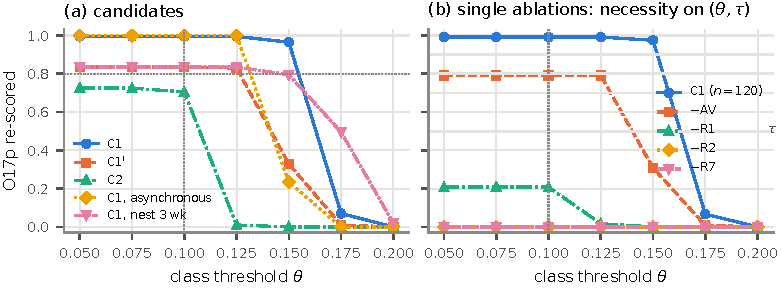
\includegraphics[width=0.8\textwidth]{fig_res_theta.pdf}
  \caption{O17p re-scored with the class threshold $\theta$ (the production value is 0.10, dotted).
  \textbf{(a)}~Candidates and two variants of \textsf{C1}. \textbf{(b)}~\textsf{C1} and its single ablations
  ($n=120$); the horizontal lines are the ensemble thresholds $\tau=0.5$--0.9 of the necessity grid.}
  \label{fig:res-theta}
\end{figure}

\subsection{Robustness variants and system size: tables}
\label{app:res-rob}

Table~\ref{tab:res-rob} lists the robustness variants of Section~\ref{sec:res-robustness} and
Table~\ref{tab:res-size} the lattice sizes at fixed density. In every variant that loses the primary outcome the
loss comes from a single criterion: O5 for the background mortality and the non-synchronous initial conditions
(and, marginally, for \textsf{C1}$'$), O11 for the nest period and for pups born above the deterioration threshold.
O5 is lost through its timing clause $(t_{B99}-t'_{\rm pk})/t'_{\rm pk}\le0.5$, not through its level clause
$N(t_{B99})\ge0.7\,N_{\rm pk}$: at $\mu_{\rm bg}=0.003$ the O5 verdicts of \textsf{C1} are 110 PASS, 83 MARGINAL and
7 FAIL (median $t'_{\rm pk}$ 29 weeks against 34 in the reference ensemble, median $t_{B99}$ 43 against 40); at
0.008, 12, 118 and 70 ($t'_{\rm pk}$ 26, $t_{B99}$ 50); with ages U\{4..80\}, 126, 73 and 1 ($t'_{\rm pk}$ 29,
$t_{B99}$ 41); with U\{4..52\}, 186, 14 and 0. The column ``disc.'' of Table~\ref{tab:res-rob} shows that the
criteria that discriminate against the null models (with O11 scored at six weeks) are untouched by the demographic variants (1.00 in every
\textsf{C1} arm with background mortality or spread ages; 0.96--0.99 in \textsf{C1}$'$) and are lost only where O11 is
lost (nest period, $s_{\rm base}>0$). Along the background-mortality curve the primary outcome is lost gradually: at
$\mu_{\rm bg}=0.001$ per week, a tenth of the senescent hazard, O17p is still 0.83. In the lattice-size stage the
failures at $L=15$ (11 of 60) and $L=20$ (6 of 60) are O5 marginal in 5 runs at each size, O11 marginal in 1 at
each, and at $L=15$ the anti-pattern A2 (recovery of natality) in 6 runs; at $L=30$ one run fails O5 and at
$L\ge45$ none fails.

\begin{figure}[ht]
  \centering
  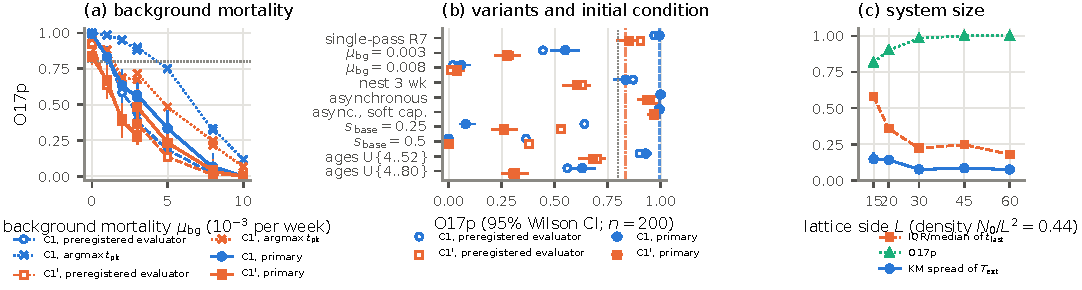
\includegraphics[width=\textwidth]{fig_res_rob.pdf}
  \caption{Robustness of the primary outcome ($n=200$ per arm unless stated).
  \textbf{(a)}~O17p against the background mortality $\mu_{\rm bg}$ for \textsf{C1} and \textsf{C1}$'$ ($n=60$ at the
  intermediate values), with the primary evaluator (filled), the preregistered evaluator (open) and with $\arg\max N$
  as peak time (crosses).
  \textbf{(b)}~Variants of \textsf{C1} and \textsf{C1}$'$: single-pass refuge admission, background mortality, nest
  period, asynchronous update with hard and soft capacity, pups born at $s_{\rm base}=0.25$ and 0.5, and initial
  ages drawn from U\{4..52\} and U\{4..80\}. Vertical lines: the reference ensembles and the 0.8 threshold.
  \textbf{(c)}~Lattice side at fixed density ($n=60$): KM spread of the extinction time, relative spread of the
  last birth and O17p.}
  \label{fig:res-rob}
\end{figure}

\begin{table}[ht]
  \centering
  \caption{Robustness variants ($n=200$ per arm). O17p with 95\% Wilson interval and Newcombe interval of the
  difference with the reference ensemble; the same arm with the preregistered evaluator and with $\arg\max N$ as peak
  time; ``disc.'': O17p restricted to the criteria that discriminate against the null models (O11 scored at six
  weeks, O13 and O13p pass and no anti-pattern is triggered), which leaves out the generic O4--O7 and O10; the criterion with the lowest
  pass rate when O17p $<0.95$ (NA counted as failure); median peak density, plateau length (weeks within 2\% of the
  maximum) and Kaplan--Meier median of $T_{\rm ext}$.}
  \label{tab:res-rob}
  \scriptsize
  \setlength{\tabcolsep}{3.2pt}
  \begin{tabular}{@{}lllccclccc@{}}
    \toprule
    Variant & O17p & $\Delta$ vs.\ reference & prereg. & $\arg\max$ & disc. & fails & $\rho_{\rm pk}$ & plateau & $T_{\rm ext}$ \\
    \midrule
    \emph{C1}, reference & 0.99 [0.97, 1.00] & -- & 0.98 & 1.00 & 1.00 & -- & 0.36 & 51 & 169 \\
single-pass R7 admission & 0.99 [0.97, 1.00] & +0.00 [-0.02, +0.02] & 0.97 & 1.00 & 1.00 & -- & 0.37 & 52 & 168 \\
$\mu_{\rm bg}=0.003$ & 0.55 [0.48, 0.62] & -0.44 [-0.51, -0.37] & 0.45 & 0.88 & 1.00 & O5 0.55 & 0.33 & 17 & 174 \\
$\mu_{\rm bg}=0.008$ & 0.06 [0.03, 0.10] & -0.94 [-0.96, -0.89] & 0.02 & 0.32 & 1.00 & O5 0.06 & 0.30 & 10 & 182 \\
nest period 3 wk & 0.83 [0.78, 0.88] & -0.16 [-0.22, -0.11] & 0.87 & 0.90 & 0.90 & O11 0.90 & 0.31 & 53 & 171 \\
asynchronous, hard & 1.00 [0.98, 1.00] & +0.01 [-0.01, +0.03] & 1.00 & 1.00 & 1.00 & -- & 0.43 & 57 & 159 \\
asynchronous, soft & 0.99 [0.97, 1.00] & +0.00 [-0.02, +0.02] & 0.99 & 0.99 & 0.99 & -- & 0.42 & 57 & 158 \\
$s_{\rm base}=0.25$ & 0.08 [0.05, 0.13] & -0.92 [-0.95, -0.86] & 0.64 & 0.07 & 0.08 & O11 0.08 & 0.40 & 53 & 164 \\
$s_{\rm base}=0.5$ & 0.00 [0.00, 0.02] & -0.99 [-1.00, -0.97] & 0.36 & 0.00 & 0.00 & O11 0.00 & 0.44 & 53 & 165 \\
ages U\{4..52\} & 0.93 [0.89, 0.96] & -0.06 [-0.11, -0.03] & 0.90 & 1.00 & 1.00 & O5 0.93 & 0.36 & 28 & 167 \\
ages U\{4..80\} & 0.63 [0.56, 0.69] & -0.36 [-0.43, -0.30] & 0.56 & 0.97 & 1.00 & O5 0.63 & 0.34 & 22 & 173 \\
\midrule
\emph{C1$'$}, reference & 0.83 [0.78, 0.88] & -- & 0.93 & 0.96 & 0.97 & -- & 0.32 & 50 & 182 \\
single-pass R7 admission & 0.85 [0.79, 0.89] & +0.02 [-0.06, +0.09] & 0.91 & 0.95 & 0.96 & O5 0.89 & 0.33 & 49 & 180 \\
$\mu_{\rm bg}=0.003$ & 0.28 [0.22, 0.34] & -0.56 [-0.63, -0.47] & 0.28 & 0.68 & 0.96 & O5 0.28 & 0.29 & 19 & 183 \\
$\mu_{\rm bg}=0.008$ & 0.04 [0.02, 0.08] & -0.79 [-0.84, -0.73] & 0.01 & 0.24 & 0.96 & O5 0.04 & 0.26 & 9 & 182 \\
nest period 3 wk & 0.60 [0.54, 0.67] & -0.23 [-0.31, -0.14] & 0.63 & 0.69 & 0.69 & O11 0.69 & 0.30 & 52 & 181 \\
asynchronous, hard & 0.94 [0.89, 0.96] & +0.10 [+0.04, +0.16] & 0.98 & 0.99 & 0.99 & O5 0.94 & 0.38 & 56 & 173 \\
asynchronous, soft & 0.97 [0.94, 0.99] & +0.14 [+0.08, +0.19] & 0.98 & 1.00 & 1.00 & -- & 0.38 & 56 & 173 \\
$s_{\rm base}=0.25$ & 0.26 [0.20, 0.32] & -0.57 [-0.65, -0.49] & 0.53 & 0.30 & 0.31 & O11 0.32 & 0.38 & 50 & 175 \\
$s_{\rm base}=0.5$ & 0.00 [0.00, 0.02] & -0.83 [-0.88, -0.77] & 0.38 & 0.01 & 0.00 & O11 0.01 & 0.43 & 47 & 174 \\
ages U\{4..52\} & 0.68 [0.61, 0.74] & -0.15 [-0.24, -0.07] & 0.70 & 0.97 & 0.99 & O5 0.69 & 0.33 & 26 & 182 \\
ages U\{4..80\} & 0.31 [0.25, 0.38] & -0.52 [-0.60, -0.44] & 0.30 & 0.77 & 0.99 & O5 0.31 & 0.30 & 21 & 187 \\
\bottomrule

  \end{tabular}
\end{table}

\begin{table}[ht]
  \centering
  \caption{Lattice side $L$ at fixed seeding density $N_0/L^2=0.44$ ($n=60$ per size, $T=600$). Medians over runs;
  $t_{\rm last}$ is the last surviving birth, $D_{\rm last}=T_{\rm ext}-t_{\rm last}$; the spread is the
  interquartile range over the median of the Kaplan--Meier estimate of $T_{\rm ext}$, with bootstrap interval.}
  \label{tab:res-size}
  \scriptsize
  \setlength{\tabcolsep}{3.5pt}
  \begin{tabular}{@{}rrrlcccrrrrl@{}}
    \toprule
    $L$ & $N_0$ & $n$ & O17p & $\rho_{\rm pk}$ & $f_0$ & $\Phi^{\rm pers}_{\rm BO}$ & $t_{\rm last}$ & IQR & $D_{\rm last}$ & $T_{\rm ext}$ & spread \\
    \midrule
    15 & 100 & 60 & 0.82 [0.70, 0.89] & 0.35 & 0.18 & 0.18 & 50 & 29 & 110 & 162 & 0.148 [0.121, 0.194] \\
20 & 178 & 60 & 0.90 [0.80, 0.95] & 0.36 & 0.17 & 0.17 & 62 & 22 & 112 & 175 & 0.143 [0.110, 0.169] \\
30 & 400 & 60 & 0.98 [0.91, 1.00] & 0.37 & 0.16 & 0.17 & 58 & 13 & 110 & 170 & 0.076 [0.053, 0.112] \\
45 & 900 & 60 & 1.00 [0.94, 1.00] & 0.37 & 0.15 & 0.17 & 66 & 16 & 111 & 176 & 0.085 [0.052, 0.113] \\
60 & 1600 & 60 & 1.00 [0.94, 1.00] & 0.37 & 0.15 & 0.17 & 75 & 14 & 110 & 184 & 0.076 [0.050, 0.103] \\
\bottomrule

  \end{tabular}
\end{table}

\subsection{Phase planes}
\label{sec:res-planes}

All planes use 30 runs per point; the 40 points nearest to a Calhoun-like boundary (9 of P1, 12 of P1-$a_w$ and 19
of P2) were re-run with 100 independent runs.

\paragraph{Socialisation: inheritance $w$ and learning rate $r$ (P1).}
With crowding damage ($\gamma=0.1$, Fig.~\ref{fig:res-planes-social}a), every one of the 56 points goes extinct
($P_{\rm ext}=1$), so the plane decides only \emph{which} collapse occurs. O17p is 0.83--1.00 for $w\le0.3$ and
$r\le0.10$. It falls in two directions, both through the primary O11: with strong inheritance ($w\ge0.5$: 0.33 at
$r=0.02$, 0 at $w\ge0.75$) the late cohorts inherit the competence of their mothers, and with fast learning
($r\ge0.2$: 0.57 at $w=0.2$, $r=0.2$; 0 at $r=0.3$ for $w\ge0.2$) they acquire it from the few competent adults.
These are point estimates with 30 runs per cell (Wilson half-width up to $\pm0.17$); the boundaries of the maps have
no intervals of their own. Without crowding damage ($\gamma=0$, panel b), colonies either explode or, in the
subcritical corner, collapse endogenously after overshooting the capacity (Q7).

\paragraph{Plasticity window $a_w$ and learning rate $r$ (P1-$a_w$).}
For every finite window up to $a_w=24$ weeks and every $r$ from 0.02 to 0.3, extinction is certain (48 of 48
points at $P_{\rm ext}=1$). O17p degrades at the fastest learning rates: at $r=0.2$ it is 0.10--0.13 for
$a_w\le8$ and 0.40--0.60 for $a_w\ge12$, and at $r=0.3$ it is at most 0.07; in every case O11 is the criterion that
fails, more often the shorter the window. The loss of the persistent class with long windows and fast learning,
which set the boundary with the preregistered evaluator (O13p 0.17 at $a_w=24$, $r=0.3$), is hidden behind O11 with the primary evaluator.
Without a window ($a_w=\infty$, top row of Fig.~\ref{fig:res-planes-social}c), recovery is again individual and
reversible: $P_{\rm ext}$ falls from 1.00 at $r=0.02$ to 0.47 at $r=0.07$ and to 0 for $r\ge0.2$, and the
anti-pattern A2 (recovery of natality) rises from 0 to 1.

\paragraph{Attraction $\alpha$ and aversion $\kappa$ (P2).}
O17p is at least 0.8 at 34 of the 48 points with $\alpha\ge2$ and at 35 of the 56 points of the plane
(Fig.~\ref{fig:res-planes-space}a). It fails in three places:
\begin{itemize}
  \item where the free space of the primary O4 is lost: at $\alpha\le2$ with $\kappa\ge0.1$, at $\alpha=3$ with
    $\kappa=0.2$ and at $\kappa=0.3$ for $\alpha\le5$, the empty fraction at the peak is below 0.10 (panel c);
  \item at $\kappa=0.3$ with $\alpha\ge5$, where in addition the crowded fraction falls to the 10\% threshold of O13
    (0.33--0.73);
  \item without aversion and with strong attraction ($\kappa=0$, $\alpha\ge5$; 0.67, 0.63 and 0.33), where O5 and
    O11 fail in a third of the runs; with 100 runs the point $(\alpha,\kappa)=(8,0)$ gives 0.53 [0.43, 0.63].
\end{itemize}
The empty fraction at the peak increases with $\alpha$ and decreases with $\kappa$ (Spearman $+0.56$ and $-0.77$,
exploratory, BH-significant; panel c). The peak density does the opposite. The coexistence band predicted for the
model without refuges is not observed in \textsf{C1} (Q5). Varying the aversion exponent at $\alpha=4$ ($p=2$ or 8)
leaves O17p at or above 0.8 except at $\kappa=0.3$ (0 and 0.30) and at $p=2$, $\kappa=0.2$ (0.47).

\paragraph{Refuges: fraction $f_R$, preference $\pi$ and capacity $c_R$ (P5).}
A persistent isolated class requires both a strong preference and a large enough total capacity: with $c_R=2$,
$\pi\ge30$ and $f_Rc_R\ge0.6$, or $\pi\ge100$ and $f_Rc_R\ge0.4$; with $c_R=1$, $\pi\ge100$ and $f_Rc_R\ge0.4$, or
$\pi=1000$ and $f_Rc_R\ge0.3$ (9 of 50 points with O13p $\ge0.8$; Fig.~\ref{fig:res-planes-space}d,e). The bound
$\Phi^{\rm pers}_{\rm BO}\le\phi_R=f_Rc_R|G|/N_{\rm pk}$ of Section~\ref{sec:model-groups} holds at all 50 points
and is approached for $\pi\ge100$ (panel f). \textsf{C1} lies at $\phi_R=0.21$, with
$\Phi^{\rm pers}_{\rm BO}=0.17$. Large capacity combined with the strongest preference degrades the senescent
decline: O8 is 0.00--0.13 at $\pi=1000$ with $f_R\ge0.2$, $c_R=2$, and O17p falls to 0.47 at $f_R=0.4$ through O5.

\paragraph{Refined boundary points.}
Over the 40 refined points the 100-run estimate differs from the 30-run estimate by 0.07 on average (mean shift
$+0.03$, maximum 0.30, correlation 0.93), the size expected from binomial sampling with 30 runs; 26 of the 40
30-run values lie within the 100-run Wilson interval. Five points crossed the 0.8 threshold, four of them upwards.
The points were selected because their 30-run estimate lay near the boundary, so part of these shifts is
regression to the mean. No conclusion of the planes changes.

\begin{figure}[ht]
  \centering
  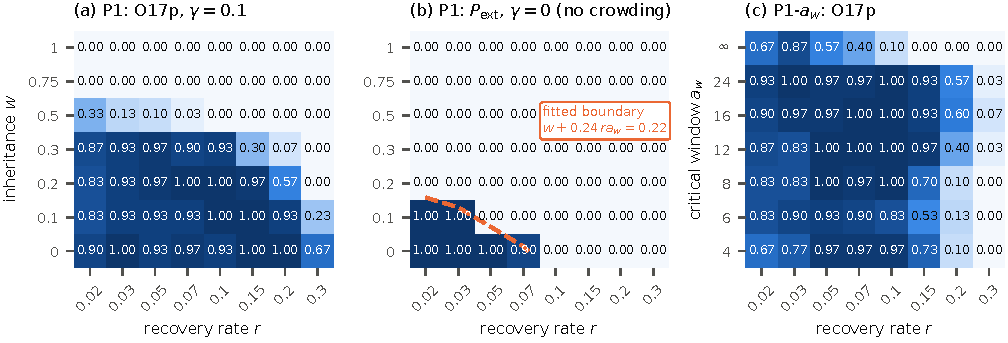
\includegraphics[width=\textwidth]{fig_res_planes_social.pdf}
  \caption{Socialisation planes around \textsf{C1} (30 runs per cell, primary evaluator).
  \textbf{(a)}~O17p in the plane of learning rate $r$ and inheritance $w$, with crowding damage $\gamma=0.1$;
  every cell goes extinct.
  \textbf{(b)}~Extinction probability in the same plane without crowding damage ($\gamma=0$); the other colonies
  explode. The dashed line is the fitted boundary $w+\hat\varphi\,r a_w=c$ of the generational map (Q7).
  \textbf{(c)}~O17p in the plane of $r$ and the critical window $a_w$. The top row ($a_w=\infty$) is \textsf{C1}
  without R1.}
  \label{fig:res-planes-social}
\end{figure}

\begin{figure}[ht]
  \centering
  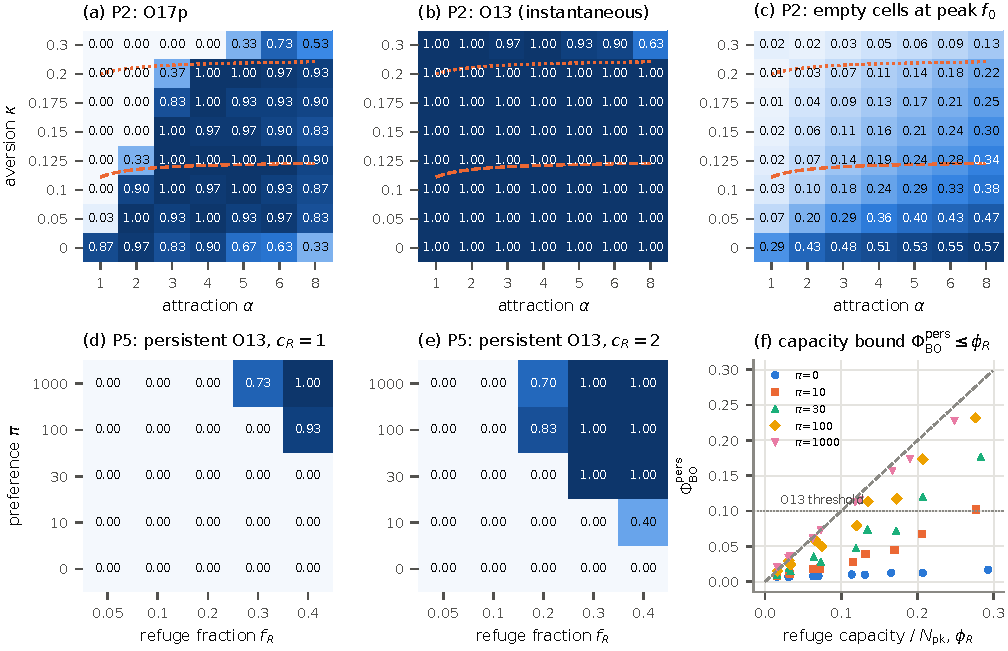
\includegraphics[width=\textwidth]{fig_res_planes_space.pdf}
  \caption{Spatial planes around \textsf{C1} (30 runs per cell, primary evaluator).
  \textbf{(a)--(c)}~Plane of attraction $\alpha$ and aversion $\kappa$ (exponent $p=4$): O17p, the instantaneous
  coexistence criterion O13, and the empty fraction at the peak. The dashed and dotted lines mark $n^*=m_c$ and
  $n^*=4$, with $n^*=1/\kappa-1/\alpha$.
  \textbf{(d, e)}~Persistent O13 in the refuge plane of fraction $f_R$ and preference $\pi$, for capacities
  $c_R=1$ and $2$.
  \textbf{(f)}~Persistent isolated fraction against the refuge capacity per individual at the peak, $\phi_R$, for
  the 50 points of (d, e). The dashed line is the bound $\Phi^{\rm pers}_{\rm BO}=\phi_R$.}
  \label{fig:res-planes-space}
\end{figure}

\subsection{Global sensitivity}
\label{sec:res-sensitivity}

Fig.~\ref{fig:res-sensitivity} reports the elementary effects of the Morris screening, over 15 factors and ranges
around \textsf{C1}, and the Sobol' indices of the 11 factors of the production design, each with its bootstrap interval
and the empirical noise floor of Section~\ref{sec:stats}. Table~\ref{tab:res-region} and Fig.~\ref{fig:res-region}
give the estimators of the Calhoun-like region of the hypercubes.

\paragraph{Noise floor.}
The split-half contrast $e=(\bar Y_{\rm even}-\bar Y_{\rm odd})/2$ of the replicate means at each design point has
expectation zero and the variance of the replicate noise, so the Morris and Sobol' estimators applied to it give the
floor below which an index is indistinguishable from noise. A factor is distinguishable in the screening if its
$\mu^*$ exceeds that of $e$ by a factor of two, and relevant for a Sobol' index if $S_T-S_T^{\rm noise}>0.05$ and the
lower confidence bound exceeds the floor; without the floor, synthetic data with three replicates and null factors
give $S_T\approx0.3$.

\paragraph{Screening.}
For O17p the largest elementary effects are those of the refuge capacity $c_R$ ($\mu^*=0.18$), the aversion
$\kappa$ (0.16), the community size $m_c$ (0.15), the conception probability $p_0$ (0.09) and the attraction
$\alpha$ (0.08); the preference $\pi$ and the inheritance $w$ follow (0.075). With the primary evaluator O17p is
zero at most Morris points, so the elementary effects are small and their bootstrap intervals are as large as the
effects. For every factor $\sigma$ is about twice $\mu^*$; because each output is an average of 10 binary runs,
$\sigma$ includes replicate noise, and without a noise floor for $\sigma$ this does not show that the factors act
through interactions. The automatic selection averages the relative $\mu^*$ over seven metrics and retained $m_c$,
$\kappa$, $\alpha$, $c_R$, $\gamma$, $w$, $\eta$ and $r$, together with the aversion exponent $p$ and $p_0$; $w$, $r$ and
$a_w$ were added by design, so the Sobol' design has 11 factors and holds four at their
\textsf{C1} values: $f_R$, $\pi$, $a_{\max}$ and $\delta$. The indices below are conditional on these four.

\paragraph{Variance decomposition.}
The Saltelli design ($N=256$, 3\,328 points, 11 factors) was run with 3 runs per point and then extended to 6
(19\,968 runs); the values below use the 6 runs. Doubling the runs halved the noise floors (median floor of $S_T$ for
O17p from 0.12 to 0.07) and changed the total indices of the continuous outputs by at most 0.01 ($\rho_{\rm pk}$,
$f_0$, $\Phi^{\rm pers}_{\rm BO}$) and those of O13 and O13p by at most 0.05; for O17p the largest change is 0.10
($m_c$ from 0.39 to 0.31, $\gamma$ from 0.26 to 0.16), and the number of factors above the floor rises from 7 to 10.
With the primary evaluator O17p is zero at 78\% of the points and at least 0.8 at 9\% (mean 0.135): the
Calhoun-like region is a minority of the box even with four parameters held at their \textsf{C1} values. For O17p
the total indices are $c_R$ $0.49\pm0.16$, $w$ $0.43\pm0.15$, $\kappa$ $0.41\pm0.14$, $r$ $0.32\pm0.12$ and $m_c$
$0.31\pm0.12$, followed by $\eta$, $\gamma$, $p$, $p_0$ and $\alpha$ (0.12--0.17, against floors of 0.05--0.09); $a_w$
(0.11) does not exceed its floor. The intervals of the five leading factors overlap, so they cannot be ordered. The
first-order indices add up to 0.15 and the total indices to 2.8: O17p is almost entirely interactions, and 31\% of
its run-level variance is within points. In the Sobol' design of the preregistered plan, which excluded $w$, $r$ and
$a_w$, $m_c$, $f_R$ and $c_R$ led; with the 11 factors, the inheritance $w$ and the aversion $\kappa$ rank with the refuge
capacity, in agreement with the hypercube regressions; with the free-space condition of O4, $\kappa$ enters through
O4 ($S_T=0.55$), and $w$ through O11 ($S_T=0.75$, $S_1=0.49$). For the persistent class O13p the leading factors
are $c_R$ (0.62), $m_c$ (0.48) and $\kappa$ (0.30), and $w$ is below the floor. Two of these are partly
definitional: with $c_R=3$ refuge residents exceed the isolation threshold of O13, so O13p averages 0.56 at $c_R=2$
against 0.11 at $c_R=1$ and 0 at $c_R=3$; and $m_c$ also defines the damage threshold, so the mean of O13 falls from
0.68 for $m_c\in(6,9]$ to 0.39 for $m_c>12$.
The continuous outputs are almost additive and dominated by the spatial and learning parameters: for the peak
density (sum of first-order indices 1.01) $r$ 0.21, $\kappa$ 0.19, $\eta$ 0.15, $\gamma$ 0.13, $a_w$ 0.10 and
$\alpha$ 0.10, every factor above a floor of 0.002; for the empty fraction (0.76) $\kappa$ 0.44, $m_c$ 0.28, $\alpha$
0.16 and $\eta$ 0.12; for $\Phi^{\rm pers}_{\rm BO}$ (0.89) $c_R$ 0.64 and $m_c$ 0.37, with no other factor above the
floor. The indices of O7 and $P_{\rm ext}$ are degenerate (98\% of the points share the same value; total indices
above one with intervals wider than one) and are not reported: over the box, extinction is generic. For the median
extinction time $m_c$ (0.66), $\kappa$ (0.32) and $p_0$ (0.30) exceed floors of about 0.1; with 3 runs per point only
the first two did.

\paragraph{Latin hypercubes.}
A Firth logistic regression of O17p on the standardised factors shows lack of fit (Pearson dispersion 2--3), so
standard errors are inflated by its square root. With this quasi-binomial correction and a false discovery rate of
10\%, the factors significant in the first hypercube are $\kappa$ ($-1.4$), $f_R$ ($+1.4$), $w$ ($-1.4$), $r$
($-1.2$), $\gamma$ ($+1.1$), $\pi$ ($+1.0$), $a_{\max}$ ($+0.8$), $\alpha$ ($+0.7$), $m_c$ ($-0.6$) and $a_w$
($+0.5$); in the second, $\kappa$ ($-1.7$), $f_R$ ($+1.1$), $m_c$ ($-1.0$), $\pi$ ($+0.9$), $p$ ($+0.8$), $w$ ($-0.7$),
$a_{\max}$ ($+0.7$), $\eta$ ($+0.6$), $p_0$ ($+0.5$) and $c_R$ ($-0.4$). The effects of $\kappa$, $f_R$, $\pi$, $w$,
$m_c$ and $a_{\max}$ replicate; those of $r$, $\gamma$, $\alpha$ and $a_w$ appear only in the first hypercube and
those of $p$, $\eta$, $p_0$ and $c_R$ only in the second (the effect of $c_R$ is non-monotone and a linear term does
not describe it). With the preregistered evaluator the leading factors were $m_c$, $f_R$, $\pi$, $w$ and $\kappa$; the
primary O4 and O5 add the aversion and the learning parameters.

\paragraph{Estimators of the Calhoun-like region.}
Table~\ref{tab:res-region} gives, for the primary evaluator, the preregistered evaluator and the fixed class threshold
alone, the naive fraction of points with $k/n\ge0.8$, the mean of O17p over the box and the empirical-Bayes
fraction, without and with the 40 extra runs at the 18 boundary points. The extra runs halve the number of
uncertain points (posterior probability between 0.05 and 0.95) from 12 to 8 and leave the estimates within their
intervals. Taking each option separately, the naive fraction is 2.0\% with the primary evaluator, 3.8\% with
$\arg\max N$ as peak time, 5.0\% with the end of the plateau, 4.2\% with the preregistered O4, 2.5\% with $m>m_c$ and
0\% with O5 on the last sustained birth; the preregistered evaluator gives 7.2\%.

\begin{table}[ht]
  \centering
  \caption{Estimators of the Calhoun-like fraction of the two 15-factor hypercubes (400 points, 10 runs each),
  relative to the box and to the sampling scales. Naive: fraction of points with $k/n\ge0.8$; volume: mean of O17p
  over the box; EB: mean posterior probability of $p_i\ge0.8$ under a beta prior centred on a logistic emulator, with
  dispersion $\phi$ fitted by beta-binomial maximum likelihood. Bootstrap intervals over points with re-fit;
  ``uncertain'': points with posterior probability between 0.05 and 0.95. The extra runs are 40 additional runs at the 18
  points with $0.4\le k/n\le0.95$ under the primary evaluator.}
  \label{tab:res-region}
  \scriptsize
  \setlength{\tabcolsep}{3.5pt}
  \begin{tabular}{@{}lllllcc@{}}
    \toprule
    Evaluator & Runs & naive & volume & EB & $\phi$ & uncertain \\
    \midrule
    primary & 10 per point & 0.022 [0.010, 0.040] & 0.041 [0.027, 0.060] & 0.015 [0.006, 0.029] & 1.22 & 12 \\
primary & +40 at 18 points & 0.020 [0.007, 0.036] & 0.040 [0.026, 0.059] & 0.018 [0.007, 0.032] & 0.82 & 8 \\
preregistered & 10 per point & 0.077 [0.052, 0.105] & 0.110 [0.082, 0.137] & 0.066 [0.045, 0.090] & 0.63 & 30 \\
preregistered & +40 at 18 points & 0.072 [0.050, 0.098] & 0.110 [0.083, 0.137] & 0.069 [0.048, 0.092] & 0.60 & 26 \\
$m>m_c$ & 10 per point & 0.028 [0.013, 0.045] & 0.054 [0.039, 0.075] & 0.020 [0.009, 0.034] & 1.00 & 17 \\
$m>m_c$ & +40 at 18 points & 0.025 [0.013, 0.043] & 0.054 [0.038, 0.073] & 0.021 [0.010, 0.035] & 0.79 & 12 \\
\bottomrule

  \end{tabular}
\end{table}

\begin{figure}[ht]
  \centering
  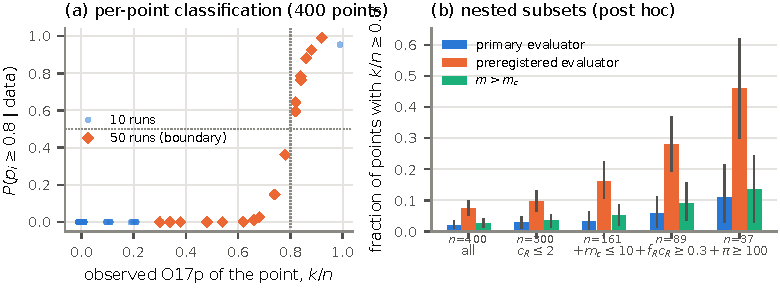
\includegraphics[width=0.8\textwidth]{fig_res_region.pdf}
  \caption{The Calhoun-like region of the hypercubes with per-point uncertainty (primary evaluator).
  \textbf{(a)}~Posterior probability that a point has $p\ge0.8$ against its observed fraction $k/n$; the 18
  boundary points with 50 runs are highlighted.
  \textbf{(b)}~Fraction of points with $k/n\ge0.8$ in nested subsets chosen after the runs ($c_R\le2$, then
  $m_c\le10$, $f_Rc_R\ge0.3$ and $\pi\ge100$), with bootstrap intervals, for the primary evaluator, the preregistered
  evaluator and the fixed class threshold alone.}
  \label{fig:res-region}
\end{figure}

\begin{figure}[ht]
  \centering
  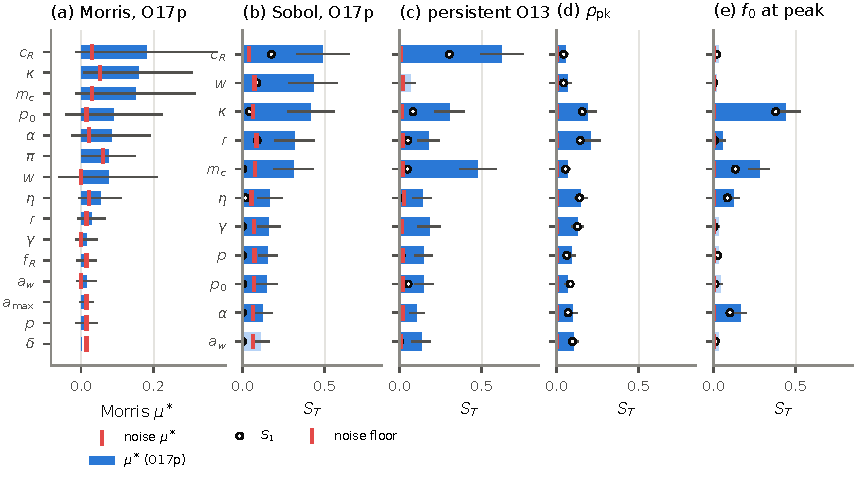
\includegraphics[width=\textwidth]{fig_res_sensitivity.pdf}
  \caption{Global sensitivity around \textsf{C1} (primary evaluator).
  \textbf{(a)}~Morris $\mu^*$ of O17p with bootstrap intervals (15 factors, $r=20$ trajectories, 10 runs per point
  with common random numbers). Red ticks: $\mu^*$ of the split-half noise contrast.
  \textbf{(b)--(e)}~Sobol' total indices $S_T$ (bars, bootstrap intervals), first-order indices $S_1$ (open
  circles) and noise floor (red ticks) for O17p, persistent O13, $\rho_{\rm pk}$ and $f_0$. Saltelli design with
  $N=256$ and 11 factors. Dark bars meet the relevance criterion $S_T-S_T^{\rm noise}>0.05$ and
  $S_T-\mathrm{CI}>S_T^{\rm noise}$.}
  \label{fig:res-sensitivity}
\end{figure}

\subsection{Seeding density, lattice size and founders}
\label{app:res-p4p6}

\paragraph{Seeding density and lattice size (P4).}
The plane combines $L=15$, 20 and 30 with $N_0=20$--800 animals of age 4 weeks placed at random, plus four founding
pairs of age 7 weeks in one cell, with 30 runs per point and the other parameters of \textsf{C1}
(Fig.~\ref{fig:res-p4}). The peak density is monotone in $N_0/L^2$ (Spearman 0.998) and rises from 0.07 to 0.94;
points with the same density have nearly the same peak density whatever $L$, which supports, without testing, that
the lattice size adds nothing at fixed density (the fixed-density stage of Section~\ref{sec:res-robustness} tests
it directly). O17p reaches 0.8 for $0.22\le N_0/L^2\le0.89$. At low densities the persistent class and the failure
of the late cohorts are lost and some colonies survive; at the highest density the peak approaches the capacity and
O4 fails. With four founding pairs the peak density is 0.07 ($L=30$) to 0.17 ($L=15$), and with mating in the Moore
neighbourhood 0.18 at $L=30$; no founder run is Calhoun-like.

\begin{figure}[ht]
  \centering
  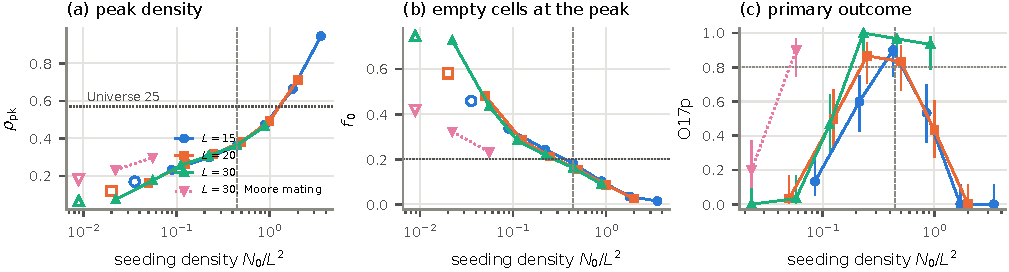
\includegraphics[width=\textwidth]{fig_res_p4.pdf}
  \caption{Seeding density and lattice size (P4; 30 runs per point). \textbf{(a)}~Peak density, \textbf{(b)}~empty
  fraction at the peak and \textbf{(c)}~O17p (95\% Wilson intervals) against the seeding density $N_0/L^2$, for
  three lattice sizes with random seeding (filled markers) and four founding pairs in one cell (open markers); the
  triangles pointing down use mating in the Moore neighbourhood. The vertical dashed line is the default initial
  condition ($N_0=400$, $L=30$); horizontal dotted lines mark the values of Universe~25 ($\rho_{\rm pk}=0.57$,
  about 20\% of empty nest boxes) and the 0.8 threshold.}
  \label{fig:res-p4}
\end{figure}

\paragraph{Founder protocol (P6).}
Four pairs of 7-week-old animals start in one cell of the $30\times30$ lattice, with mating in the Moore
neighbourhood, $T=900$ and 30 runs per point. The plane varies the initial social state of the founders $s_0$ (0.2,
0.3, 0.5; a value below one represents adaptation to the new enclosure), the number of movement sub-steps per week
$k$ (1, 2) and the longevity $a_{\max}$ (120, 200; with $a_{\max}=200$ the fertile window is extended to 133 weeks).
Table~\ref{tab:res-p6} lists the outcomes. The latency pattern O1 passes in up to 0.67 of the runs, but O1--O3
jointly with O17p pass in at most 0.43 [0.27, 0.61] ($s_0=0.2$, $k=1$, $a_{\max}=200$). The best points need
$a_{\max}=200$, outside the preset; with $a_{\max}=120$ no point exceeds 0.13. The peak density stays at 0.16--0.27.

\begin{table}[ht]
  \centering
  \caption{Founder protocol (P6): four pairs in one cell with mating in the Moore neighbourhood, 30 runs per point.
  $s_0$ is the initial social state of the founders and $k$ the number of movement sub-steps per week. O1--O3 is
  the fraction of runs that pass the latency, growth and deceleration patterns jointly; O17p with 95\% Wilson
  interval.}
  \label{tab:res-p6}
  \small
  \begin{tabular}{@{}cccccccccc@{}}
    \toprule
    $s_0$ & $k$ & $a_{\max}$ & O1 & O1--O3 & O17p & O13p & $P_{\rm ext}$ & $\rho_{\rm pk}$ & $f_0$ \\
    \midrule
    0.2 & 1 & 120 & 0.53 & 0.47 & 0.13 [0.05, 0.30] & 0.64 & 0.63 & 0.18 & 0.43 \\
0.2 & 1 & 200 & 0.67 & 0.63 & 0.43 [0.27, 0.61] & 0.80 & 0.93 & 0.23 & 0.33 \\
0.2 & 2 & 120 & 0.57 & 0.23 & 0.13 [0.05, 0.30] & 0.54 & 1.00 & 0.16 & 0.51 \\
0.2 & 2 & 200 & 0.63 & 0.43 & 0.23 [0.12, 0.41] & 0.74 & 1.00 & 0.18 & 0.46 \\
0.3 & 1 & 120 & 0.47 & 0.47 & 0.10 [0.03, 0.26] & 0.72 & 0.67 & 0.20 & 0.38 \\
0.3 & 1 & 200 & 0.43 & 0.43 & 0.33 [0.19, 0.51] & 0.83 & 0.97 & 0.24 & 0.30 \\
0.3 & 2 & 120 & 0.57 & 0.40 & 0.17 [0.07, 0.34] & 0.54 & 1.00 & 0.21 & 0.37 \\
0.3 & 2 & 200 & 0.37 & 0.30 & 0.23 [0.12, 0.41] & 0.80 & 1.00 & 0.27 & 0.24 \\
0.5 & 1 & 120 & 0.00 & 0.00 & 0.00 [0.00, 0.11] & 0.60 & 0.53 & 0.20 & 0.38 \\
0.5 & 1 & 200 & 0.03 & 0.03 & 0.03 [0.01, 0.17] & 0.90 & 0.87 & 0.24 & 0.29 \\
0.5 & 2 & 120 & 0.10 & 0.10 & 0.03 [0.01, 0.17] & 0.80 & 1.00 & 0.26 & 0.24 \\
0.5 & 2 & 200 & 0.23 & 0.23 & 0.10 [0.03, 0.26] & 0.93 & 1.00 & 0.27 & 0.23 \\
\bottomrule

  \end{tabular}
\end{table}

\subsection{Transplant experiments}
\label{sec:res-transplant}

Each of the 60 replicates per arm runs a mother colony and samples it at several times (Fig.~\ref{fig:res-transplant},
Tables~\ref{tab:res-trans} and~\ref{tab:res-trans-s}): in phase B; at $1.75\,t'_{\rm pk}$ (phase D of the primary
evaluator); at $1.75\,t_{\rm pk}$ with $t_{\rm pk}=\arg\max N$ (the preregistered protocol); at week 95 in every arm,
which removes the confound between rule and sampling time; and, not preregistered, at the first week in which
four males and four females past the plasticity window have $0.2\le s\le0.5$ (the ``band''). Four males and four
females are moved to an empty lattice; success is reaching 80 individuals within 150 weeks. In the mixed phases the
animals of one sex are paired with healthy animals of the other. Arm $X$ shares its mother colonies and its
transplanted animals with \textsf{C1} and places them in an enclosure without R1 and R2 with $r=0.1$.
\begin{itemize}
  \item \emph{Healthy controls.} Animals taken in phase B found colonies in 77--98\% of the trials in every arm.
  \item \emph{Phase-D animals under R1.} Whenever R1 is present (\textsf{C1}, \textsf{C1}$'$, \textsf{C0},
    \textsf{C2} and $-$R2), phase-D animals never found a colony at any of the three sampling times, nor with
    healthy partners (0/120 at week 95 in \textsf{C1}, \textsf{C1}$'$, \textsf{C0} and $-$R2; 3/120 in \textsf{C2}).
    Their social state is 0 (median), with all eight below $10^{-3}$ in 55--93\% of the trials.
  \item \emph{Without R1.} At week 60 the same test gives 0/60 in the arms without R1 too, because their colonies
    are still at the peak and the animals are young but fully deteriorated; at $1.75\,t_{\rm pk}$ (weeks 126--131)
    10/60 recover alone in $-$R1 and 3/60 in $-$R1$-$R2, and with healthy partners 34/120 and 14/120 at week 95. In
    arm $X$ the rates are 51/60 at week 60, 12/60 at week 97 and 5/60 at week 95: the recovery of the same
    animals is a matter of the fertile time left.
  \item \emph{Intermediate animals.} Band animals (weeks 8--11, ages 12--15, $s=0.33$--0.40) found colonies in
    5/60 (\textsf{C1}), 2/60 (\textsf{C1}$'$), 0/60 (\textsf{C0}), 7/60 ($-$R2) and 8/60 (\textsf{C2}) under R1,
    against 50/60 without R1, 46/60 without R1 and R2 and 57/60 in arm $X$. With healthy partners the arms with R1
    reach 35--46/60 (band males with healthy females) and 7--32/60 (band females with healthy males); the asymmetry
    follows from the fecundity $s_f^2s_m$. The equal-time comparisons between arms (Fisher, BH at 10\%) separate the
    arms with R1 from those without it in the band phases and in the mixed phases at week 95, and nothing else.
  \item \emph{Descendants of the band.} In the colonies founded by band animals, the adult descendants have a mean
    social state of 0.28--0.45 in \textsf{C1}, 0.26--0.42 in \textsf{C1}$'$, 0.11--0.35 in \textsf{C0} and
    0.33--0.37 in arms $X$ and $-$R1: in a small uncrowded colony the offspring learn the competence of their
    parents and stay there, with or without R1. The lineage criterion of Section~\ref{sec:meanfield} is therefore
    confirmed only in its first part, the founding bottleneck.
\end{itemize}
This reproduces Marsden's observation, reported by Calhoun~\cite{Calhoun1973}: animals removed in mid-phase D failed
to reproduce ``even placing them with adequate sex partners'' raised without crowding. The model reproduces it only
with R1, and by construction. The evaluator rates O12 as PASS in every arm with R1 and in $-$R1$-$R2, and as
MARGINAL in $-$R1 and arm $X$ when sampled at $1.75\,t_{\rm pk}$.

\paragraph{Transplant grid.}
Over 12 points of the plane $(\alpha,\kappa)$, with $\alpha\in\{2,4,6,8\}$ and $\kappa\in\{0.1,0.15,0.2\}$ and 40
transplants per point and phase, no phase-D transplant founded a colony (0/480), nor did any mixed transplant
(0/960). Phase-B transplants succeed in 0.63--1.00 of the trials, less often with stronger attraction (mean 0.97 at
$\alpha=4$ and 0.71 at $\alpha=8$), and O12 passes at all 12 points.

\begin{figure}[ht]
  \centering
  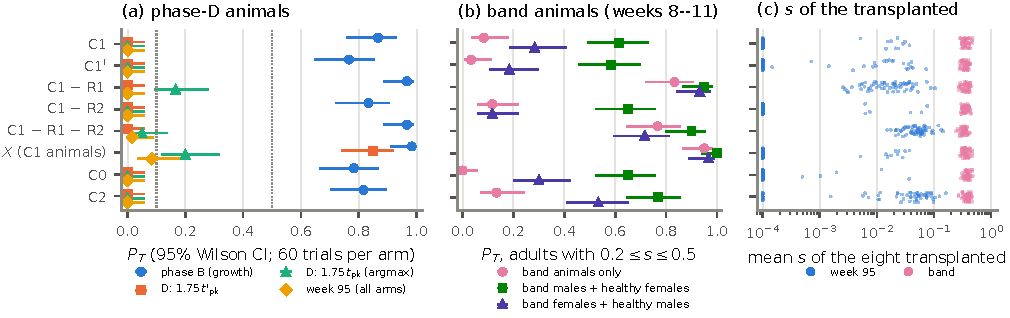
\includegraphics[width=\textwidth]{fig_res_transplant.pdf}
  \caption{Transplant experiments (60 replicates per arm and phase). $P_T$ is the probability that four males and
  four females moved to an empty lattice reach 80 individuals within 150 weeks.
  \textbf{(a)}~Animals taken in phase B and in phase D at three sampling times: $1.75\,t'_{\rm pk}$ of each colony,
  $1.75\,t_{\rm pk}$ with $t_{\rm pk}=\arg\max N$, and week 95 in every arm.
  \textbf{(b)}~Adults past the plasticity window with $0.2\le s\le0.5$, alone and paired with healthy animals of the
  other sex.
  \textbf{(c)}~Mean social state of the eight transplanted animals per trial, at week 95 and in the band.
  Arm $X$ moves the animals of the \textsf{C1} arm, the same individuals, into an enclosure without R1 and R2 with
  individual recovery at $r=0.1$. Dotted lines in (a) mark the O12 thresholds (0.1 and 0.5).}
  \label{fig:res-transplant}
\end{figure}

\begin{table}[ht]
  \centering
  \caption{Transplants that found a colony, by arm and phase (successes/trials; 60 replicates per arm). Phase D is
  sampled at $1.75\,t'_{\rm pk}$ (median sampling week in parentheses), then at $1.75\,t_{\rm pk}$ with
  $t_{\rm pk}=\arg\max N$, and at week 95 in every arm; ``+healthy (95)'' pools the two mixed phases at week 95
  (h.: healthy partners of the other sex). The band samples eight adults past the
  plasticity window with $0.2\le s\le0.5$ at the first week in which they exist (median week in parentheses), alone
  or with healthy partners of the other sex.}
  \label{tab:res-trans}
  \scriptsize
  \setlength{\tabcolsep}{4pt}
  \begin{tabular}{@{}lcccccccc@{}}
    \toprule
    Arm & B & D & $1.75\,t_{\rm pk}$ & week 95 & +healthy (95) & band & band M + h.\ F & band F + h.\ M \\
    \midrule
    C1 & 52/60 & 0/60 (60) & 0/60 & 0/60 & 0/120 & 5/60 (9) & 37/60 & 17/60 \\
C1$'$ & 46/60 & 0/60 (63) & 0/60 & 0/60 & 0/120 & 2/60 (8) & 35/60 & 11/60 \\
C1 $-$ R1 & 58/60 & 0/60 (86) & 10/60 & 0/60 & 34/120 & 50/60 (9) & 57/60 & 56/60 \\
C1 $-$ R2 & 50/60 & 0/60 (65) & 0/60 & 0/60 & 0/120 & 7/60 (10) & 39/60 & 7/60 \\
C1 $-$ R1 $-$ R2 & 58/60 & 0/60 (82) & 3/60 & 1/60 & 14/120 & 46/60 (9) & 54/60 & 43/60 \\
$X$ (C1 animals) & 59/60 & 51/60 (60) & 12/60 & 5/60 & 41/120 & 57/60 (9) & 60/60 & 58/60 \\
C0 & 47/60 & 0/60 (58) & 0/60 & 0/60 & 0/120 & 0/60 (11) & 39/60 & 18/60 \\
C2 & 49/60 & 0/60 (110) & 0/60 & 0/60 & 3/120 & 8/60 (10) & 46/60 & 32/60 \\
\bottomrule

  \end{tabular}
\end{table}

\begin{table}[ht]
  \centering
  \caption{Social state and age of the transplanted animals, by arm and phase: median over trials of the per-trial
  median $s$ of the eight animals / maximum $s$ over all trials; median over trials of the youngest and oldest
  animal (weeks). Last column: mean social state of the adult descendants (age $\ge a_w$) in the colonies founded by
  band animals, pooled over the three band phases and weighted by their number (in parentheses).}
  \label{tab:res-trans-s}
  \scriptsize
  \setlength{\tabcolsep}{4pt}
  \begin{tabular}{@{}lcccccccc@{}}
    \toprule
    & \multicolumn{2}{c}{D ($1.75\,t'_{\rm pk}$)} & \multicolumn{2}{c}{week 95} & \multicolumn{2}{c}{band} & descendants \\
    \cmidrule(lr){2-3}\cmidrule(lr){4-5}\cmidrule(lr){6-7}
    Arm & $s$ med./max & ages & $s$ med./max & ages & $s$ med./max & ages & $\bar s$ ($n$) \\
    \midrule
    C1 & 0.000 / 0.36 & 37--64 & 0.000 / 0.30 & 65--80 & 0.358 / 0.50 & 13--13 & 0.31 (10261) \\
C1$'$ & 0.000 / 0.60 & 40--66 & 0.000 / 0.49 & 60--80 & 0.354 / 0.50 & 12--12 & 0.27 (8156) \\
C1 $-$ R1 & 0.003 / 0.37 & 46--78 & 0.004 / 0.46 & 56--80 & 0.361 / 0.50 & 13--13 & 0.36 (39369) \\
C1 $-$ R2 & 0.000 / 1.00 & 40--67 & 0.000 / 0.61 & 59--80 & 0.362 / 0.50 & 14--14 & 0.19 (10131) \\
C1 $-$ R1 $-$ R2 & 0.025 / 0.80 & 47--78 & 0.028 / 0.81 & 52--80 & 0.330 / 0.46 & 13--13 & 0.23 (31128) \\
$X$ (C1 animals) & 0.000 / 0.36 & 37--64 & 0.000 / 0.30 & 65--80 & 0.358 / 0.50 & 13--13 & 0.32 (38964) \\
C0 & 0.000 / 0.60 & 36--58 & 0.000 / 0.29 & 66--80 & 0.396 / 0.50 & 15--15 & 0.11 (7448) \\
C2 & 0.000 / 0.63 & 30--79 & 0.000 / 0.71 & 28--79 & 0.398 / 0.50 & 14--14 & 0.35 (17350) \\
\bottomrule

  \end{tabular}
\end{table}

\subsection{\textsf{C1} versus \textsf{C2}}
\label{app:res-c1c2}

Table~\ref{tab:res-QC} lists the confirmatory contrast; 13 of the 29 rows differ after Holm adjustment with the
primary evaluator, 12 with the preregistered evaluator (O4 and O13p differ only with the primary O4 and the fixed class
threshold). The 29 rows hold 27 distinct tests: O6, O7 and A2 (recovery of natality) are decided by the same four \textsf{C2}
colonies, which survive to $T$ and recover natality, and in the production runs O17 and O17p differ (0.725 against 0.705). Nine rows are constant in both
arms and enter the Holm sequence with $p=1$, so the correction over 29 is conservative. Besides the losses in O8 and O9, natality collapse weakens in \textsf{C2}: O5 passes in 0.815 against
0.98, because its births are spread over a longer growth phase ($t'_{\rm pk}=62$ weeks, $t_{B99}=86$). Four of its
200 colonies persist to $T$ (A2 in 0.02). The decline is as long as in \textsf{C1}, $(T_{\rm ext}-t_{\rm pk})/t_{\rm
pk}\approx1.9$--2.1, so O8 fails because the mean age no longer rises at the required rate. The isolated class is
slightly smaller in \textsf{C2} ($\Phi^{\rm pers}_{\rm BO}=0.13$ against 0.17), the peak higher (0.42 against 0.36),
the empty fraction smaller (0.11 against 0.16) and extinction later (Kaplan--Meier median 218 against 169 weeks).

Fig.~\ref{fig:res-cohorts} shows the cohort structure behind O13b. In \textsf{C2} the isolated class is born later
than the crowded class in every run (median birth week 22 against 11), whereas in \textsf{C1} the two classes are
born together (10 against 11 weeks; the isolated class is later in 4\% of the runs): the isolated animals of
\textsf{C1} are refugees of the early boom, of the same cohorts as the crowded ones. In both candidates births are
front-loaded: half of the births of \textsf{C1} occur before $0.36\,t'_{\rm pk}$ and 93\% before $0.8\,t'_{\rm pk}$,
the start of the window used by the strict O13b criterion, which therefore cannot pass.

\begin{figure}[ht]
  \centering
  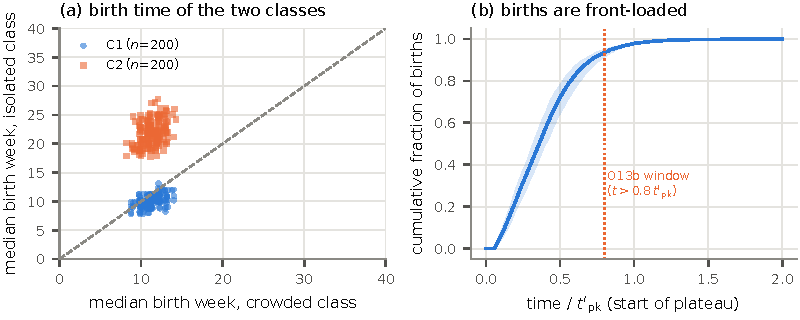
\includegraphics[width=0.8\textwidth]{fig_res_cohorts.pdf}
  \caption{Cohort structure of the deteriorated classes. \textbf{(a)}~Per-run median birth week of the persistent
  isolated class against that of the crowded class, at the time $t^*$ used by O13b, for \textsf{C1} and
  \textsf{C2} ($n=200$ each, jittered); the dashed line is the diagonal. \textbf{(b)}~Cumulative fraction of births
  against time in units of $t'_{\rm pk}$ for the \textsf{C1} reference ensemble (median and 10--90\% band over
  runs); the dotted line marks the start of the O13b window.}
  \label{fig:res-cohorts}
\end{figure}

\begin{table}[ht]
  \centering
  \caption{Confirmatory contrast between \textsf{C1} and \textsf{C2} ($n=200$ each, $T=700$; primary evaluator).
  Binary patterns are compared with two-sided Fisher tests, continuous magnitudes with Mann--Whitney tests, and
  $T_{\rm ext}$ with a log-rank test with censoring. Holm correction is applied over the 29 comparisons. Entries
  are fractions of passing runs, or medians, with the number of applicable runs in parentheses. The last column
  gives the two fractions and the verdict with the preregistered evaluator. Omitted rows show no difference: O10, O13
  and O14 pass in every run of both arms; O15, A1, A3 and A4 are identical in both arms; O8b, O11b and strict O13b
  are constant.}
  \label{tab:res-QC}
  \footnotesize
  \setlength{\tabcolsep}{4pt}
  \begin{tabular}{@{}lccllcl@{}}
    \toprule
    Pattern / magnitude & \textsf{C1} & \textsf{C2} & $p$ & $p_{\rm Holm}$ & Differs & prereg.\ evaluator \\
    \midrule
    O4 & 1.000 (200) & 0.900 (200) & $1.2\times10^{-6}$ & $2.2\times10^{-5}$ & \textbf{yes} & 1.00 / 1.00 no \\
O5 & 0.980 (200) & 0.815 (200) & $2.3\times10^{-8}$ & $4.7\times10^{-7}$ & \textbf{yes} & 1.00 / 0.90 yes \\
O6 & 1.000 (200) & 0.980 (200) & 0.12 & 1.00 & no & 1.00 / 0.98 no \\
O7 & 1.000 (200) & 0.980 (200) & 0.12 & 1.00 & no & 1.00 / 0.98 no \\
O8 & 0.645 (200) & 0.000 (196) & $<10^{-16}$ & $<10^{-16}$ & \textbf{yes} & 0.65 / 0.00 yes \\
O9 & 0.400 (200) & 0.300 (200) & 0.0462 & 0.74 & no & 0.40 / 0.30 no \\
O11 & 1.000 (200) & 0.995 (197) & 0.50 & 1.00 & no & 0.99 / 0.99 no \\
O13p & 1.000 (200) & 0.945 (200) & $8.5\times10^{-4}$ & 0.014 & \textbf{yes} & 1.00 / 1.00 no \\
O15b & 0.650 (200) & 0.452 (197) & $8.2\times10^{-5}$ & 0.0015 & \textbf{yes} & 0.65 / 0.45 yes \\
O17 & 0.980 (200) & 0.725 (200) & $4.0\times10^{-14}$ & $8.7\times10^{-13}$ & \textbf{yes} & 0.99 / 0.88 yes \\
O17p & 0.980 (200) & 0.705 (200) & $1.6\times10^{-15}$ & $3.8\times10^{-14}$ & \textbf{yes} & 0.99 / 0.88 yes \\
O13b (PASS or MARG.) & 0.000 (200) & 1.000 (200) & $<10^{-16}$ & $<10^{-16}$ & \textbf{yes} & 0.00 / 1.00 yes \\
A2 & 0.000 (200) & 0.020 (200) & 0.12 & 1.00 & no & 0.00 / 0.02 no \\
$\rho_{\rm pk}$ (median) & 0.361 (200) & 0.42 (200) & $<10^{-16}$ & $<10^{-16}$ & \textbf{yes} & yes \\
$f_0$ (median) & 0.163 (200) & 0.113 (200) & $<10^{-16}$ & $<10^{-16}$ & \textbf{yes} & yes \\
$\Phi^{\rm pers}_{\rm BO}$ (median) & 0.174 (200) & 0.133 (200) & $<10^{-16}$ & $<10^{-16}$ & \textbf{yes} & yes \\
$(T_{\rm ext}-t_{\rm pk})/t_{\rm pk}$ (extinct) & 2.06 (200) & 1.8 (196) & $3.9\times10^{-14}$ & $8.7\times10^{-13}$ & \textbf{yes} & yes \\
$T_{\rm ext}-t_{\rm last}$ (extinct) & 110 (200) & 110 (196) & 0.37 & 1.00 & no & no \\
$T_{\rm ext}$ (KM median; log-rank) & 169 (200) & 218 (200) & $<10^{-16}$ & $<10^{-16}$ & \textbf{yes} & yes \\
\bottomrule

  \end{tabular}
\end{table}

\subsection{Ensembles}
\label{app:res-ensembles}

Table~\ref{tab:res-ensembles} lists every ensemble of the production program with its size, horizon and base seed, so
that each number of the text can be traced to its source. Seeds are derived as
\texttt{SeedSequence([base\_seed, point, replicate])}; the base seeds of the production runs (25301--25336) differ from those
of the runs of the preregistered design, so the two sets of runs are independent.

\begin{table}[ht]
  \centering
  \caption{Ensembles of the production program (\texttt{results\_v2/f2b\_<stage>}). Points: design points or arms;
  per point: runs or transplant replicates; $T$: horizon in weeks; seed: base seed of the stage.}
  \label{tab:res-ensembles}
  \scriptsize
  \setlength{\tabcolsep}{4pt}
  \begin{tabular}{@{}llrrrrrl@{}}
    \toprule
    Stage & Content & points & per point & runs & $T$ & seed & used for \\
    \midrule
    \texttt{base} & reference ensemble: C1, C1$'$, C0, $\alpha=0$ & 4 & 200 & 800 & 600 & 25301 & production \\
\texttt{c1c2} & C1 and C2 & 2 & 200 & 400 & 700 & 25318 & QC \\
\texttt{ref} & short-lived and long-lived controls & 2 & 100 & 200 & 1000 & 25302 & Q3, controls \\
\texttt{nulos} & four null models & 4 & 200 & 800 & 600 & 25330 & discrimination \\
\texttt{abl1} & single ablations and variants & 9 & 120 & 1080 & 600 & 25303 & Q2 \\
\texttt{abl2} & double to quadruple ablations, $\gamma=0$ & 12 & 40 & 480 & 600 & 25304 & ablations \\
\texttt{trans} & 8 transplant arms, 11 phases & 8 & 60 & 480 & 300 & 25306 & Q1, O12 \\
\texttt{amax} & $a_{\max}\in\{90,\dots,150\}$ & 5 & 60 & 300 & 600 & 25305 & Q4 \\
\texttt{rob} & demographic and update variants & 16 & 200 & 3200 & 700 & 25331 & robustness \\
\texttt{ci} & non-synchronous initial condition & 4 & 200 & 800 & 700 & 25333 & robustness \\
\texttt{size} & $L\in\{15,\dots,60\}$ at fixed density & 5 & 60 & 300 & 600 & 25334 & size \\
\texttt{q7aw} & $a_w$ varied at $\gamma=0$ & 54 & 20 & 1080 & 600 & 25335 & Q7 \\
\texttt{p1} & plane $(r,w)\times\gamma$ & 112 & 30 & 3360 & 600 & 25309 & Q7, P1 \\
\texttt{p1aw} & plane $(r,a_w)$ & 56 & 30 & 1680 & 600 & 25310 & Q6 \\
\texttt{p2} & plane $(\alpha,\kappa)$, $p$ & 72 & 30 & 2160 & 600 & 25308 & Q5, P2 \\
\texttt{p5} & refuge plane & 50 & 30 & 1500 & 600 & 25311 & P5 \\
\texttt{lhs} & Latin hypercube 1 & 200 & 10 & 2000 & 400 & 25312 & global \\
\texttt{lhs2} & Latin hypercube 2 & 200 & 10 & 2000 & 400 & 25313 & global \\
\texttt{lhsx} & boundary points of the hypercubes & 18 & 40 & 720 & 400 & 25336 & global \\
\texttt{morris} & Morris screening & 320 & 10 & 3200 & 400 & 25307 & global \\
\texttt{sobol} & Saltelli design, 11 factors & 3328 & 6 & 19968 & 400 & 25314 & global \\
\texttt{robmu} & $\mu_{\rm bg}$ curve & 12 & 60 & 720 & 700 & 25332 & robustness \\
\texttt{p4} & seeding density and lattice & 24 & 30 & 720 & 600 & 25315 & P4 \\
\texttt{trgrid} & transplants on $(\alpha,\kappa)$ & 12 & 40 & 480 & 300 & 25316 & O12 \\
\texttt{refine} & 40 boundary points of the planes & 40 & 100 & 4000 & 600 & 25317 & planes \\
\texttt{p6} & founder protocol & 12 & 30 & 360 & 900 & 25319 & O1--O3 \\
\bottomrule

  \end{tabular}
\end{table}

\subsection{Deviations from the preregistration}
\label{app:res-deviations}

\begin{table}[ht]
\centering
\caption{Deviations from the preregistered plan (\texttt{docs/preregistered\_plan.md}, dated 1 October 2026, 22:02 UTC,
before the production runs) and post hoc
analyses. ``Before production'' means after the calibration but before the production runs; ``post hoc'' means
after the runs had been seen. The last block lists the changes that are not preregistered but were fixed, with their decision rules, before
the production runs (\texttt{docs/production\_plan.md}, 2 October 2026, 05:34 UTC).}
\label{tab:deviations}
\scriptsize
\setlength{\tabcolsep}{3pt}
\begin{tabular}{@{}p{4.9cm}p{2.6cm}p{4.3cm}p{3.7cm}@{}}
\toprule
Change & When & Affects & Treatment \\
\midrule
O13p (persistent isolated class) defined and made part of the primary outcome, together with R7 & before
production, after seeing that \textsf{C0} has no persistent class & O17p, Q2, necessity of R7 & declared as
circular for R7 (Section~\ref{sec:discussion}) \\
O6: rebound count also detects slow regrowth still rising at censoring & post hoc (2 Oct., 02:44) & one
\textsf{C1} run of 200 under the preregistered design; none in the production runs & primary evaluator \\
O13b: reading of the window against the median birth week (Fig.~\ref{fig:res-cohorts}) & post hoc & the
interpretation of O13b in \textsf{C1} and \textsf{C2} & labelled post hoc \\
Robust spread of $T_{\rm ext}$ (Kaplan--Meier interquartile range over median) & post hoc (the plan
had $\mathrm{CV}\le0.10$ for Q3) & the claims about the spread of the extinction time & labelled post hoc; the
equivalence of \textsf{C1}$'$ with the long-lived control found under the preregistered design does not hold in the production runs \\
Ensembles of \textsf{C1}$'$ and the \textsf{C1}--\textsf{C1}$'$ contrast & post hoc & minimality, the role of
AV & labelled post hoc \\
Subsets of the hypercubes (nested conditions on $c_R$, $m_c$, $f_Rc_R$, $\pi$) & post hoc & interpretation of the
Calhoun-like fraction & descriptive only \\
Re-scoring with other class thresholds $\theta$ and ensemble thresholds $\tau$ (Appendix~\ref{app:res-threshold}) &
post hoc & conditionality of minimality & descriptive only \\
Cure model for the extinction time & post hoc & survival summaries & no test reported \\
Holm $p$-value of Q6 computed from the binomial likelihood & as planned & Q6 & the quasi-binomial value enters the
Holm sequence; no decision changes \\
\midrule
\multicolumn{4}{@{}l}{\emph{Not preregistered, fixed before the production runs}}\\
Hard refuge capacity enforced strictly (pups and rejected movers counted); the single-pass admission kept as a variant &
before the production runs & every stage with refuges; all stages run with seeds different from those of the preregistered design & both admission rules reported side by side
(no change in O17p) \\
Primary evaluator redefined: peak time at the start of the plateau ($t'_{\rm pk}$); end of natality in O5 at 99\%
of the births; O4 also requires free space at the peak ($f_0\ge0.10$, an informal target of the calibration);
crowded class $m>8$, independent of $m_c$; O10 on the adult social state; O11 on the second half of the births, not
applicable when the late cohorts are empty; NA counts as failure in O17p & fixed after exploratory runs with the primary evaluator and before the production runs & every pattern
normalised by $t_{\rm pk}$, O4, O5, O10, O11, O13, O13p, O17p in every stage; the verdicts of Q1 (prediction), Q2
(null) and Q6 (prediction) & the full preregistered evaluator, and each option changed separately, reported next to the
primary one (Appendix~\ref{app:res-rescoring}) \\
O5 birth reference $t_{B99}$ instead of the last sustained birth $t_{\rm last}$ & after exploratory runs had
shown that $t_{\rm last}$ with $t'_{\rm pk}$ fails O5 in most \textsf{C1} runs (0.48 in the production runs,
Table~\ref{tab:res-rescoring}); a choice informed by the result & Q2: it is the only option on which the rejection
of its null hypothesis depends (with the preregistered evaluator 5 of 7 null hypotheses are rejected and Q2 is not;
with the primary one, 6 of 7) & both birth references reported for every arm; the count with the preregistered
evaluator given next to the primary one (Section~\ref{sec:res-Q}) \\
Confirmatory test of the equivalence of the exponents of $r$ and $a_w$ at $\gamma=0$ (TOST, margin $[2/3,3/2]$,
stage $a_w$ varied) & before the production runs & Q7 with $a_w$ varied & the design cannot carry it out as inference
(51 of 54 points at $P_{\rm ext}\in\{0,1\}$, separated logistic); replaced by a non-parametric summary per window
(Table~\ref{tab:res-q7aw}); the planned estimates are kept, labelled, in \texttt{results\_numbers.json} \\
O8 (senescent decline) of \textsf{C1}: 0.71 under the preregistered design, 0.62 in the production runs (0.64 with the
single-pass admission and the seeds of the production runs) & observed after the production runs & a desirable pattern; no
decision & reported; not a conclusion \\
Transplant of Q1 taken at $1.75\,t'_{\rm pk}$ instead of $1.75\,t_{\rm pk}$; sampling at a common week added &
before the production runs & Q1, O12 & both times reported; comparisons between arms only at equal time \\
Sobol' design with 11 factors (the 8 selected by Morris plus $w$, $r$, $a_w$) & before the production runs & global
sensitivity & indices conditional on the 4 fixed factors \\
Additional stages: null models, demographic and update variants, non-synchronous initial condition, transplants of
intermediate animals, extra replicates at the hypercube boundary, $a_w$ varied at $\gamma=0$ (additional confirmatory test), lattice size & before the production runs & robustness, discrimination, Q1, Q7, feasible region & decision rules fixed before the runs \\
\bottomrule
\end{tabular}
\end{table}

\section{Calibration details}
\label{app:calib}

This appendix collects the development ensembles of Section~\ref{sec:calib}. They used independent seeds and
smaller samples than the production ensembles of Section~\ref{sec:results}, which supersede them wherever the two
overlap.

\subsection{Procedure}
\label{app:calib-procedure}

\paragraph{Transplants.}
The transplant patterns O12 and O12b are ensemble experiments.
\begin{itemize}
  \item From each replicate colony, four reproductive males and four reproductive females are moved to an
    empty lattice: either from the middle of the growth window (control, phase~B) or at
    $t=1.75\,t_{\rm pk}$ (mid-phase~D).
  \item In O12b, four phase-D animals of one sex are paired with four healthy animals ($s=1$) of the other.
  \item A transplant ``founds'' a colony if it reaches 80 individuals within 150 weeks.
\end{itemize}

\paragraph{Ensembles.}
The calibration proceeded in stages:
\begin{enumerate}
  \item screening of rule families: 23 points $\times$ 10 replicates, then 24 points (initial condition
    $\times\,\alpha\times\kappa$) $\times$ 10 replicates;
  \item ablations of the selected rules: 10 points $\times$ 40 replicates;
  \item one-at-a-time sensitivity around the selected point: 17 points $\times$ 30 replicates;
  \item final ensembles: \textsf{C0} with 120 replicates, 100 transplants and an $\alpha=0$ control;
    \textsf{C1} and \textsf{C2} with 60 replicates and 60 transplants each;
  \item exploratory tests of the founder protocol: 30--60 replicates per point.
\end{enumerate}
Further details:
\begin{itemize}
  \item replicates use independent seeds, \texttt{SeedSequence([base\_seed, point, replicate])};
  \item the horizon is $T=600$ weeks, and every run of the final ensembles of \textsf{C0} and \textsf{C1}
    went extinct before week 220;
  \item a run of \textsf{C0} costs about 1~s of CPU;
  \item the whole calibration used about 45~min on four cores.
\end{itemize}

\subsection{Development ensembles of the candidates}
\label{app:calib-dev}

Table~\ref{tab:calib-dev} reports every pattern in the development ensembles of \textsf{C0}, \textsf{C1} and
\textsf{C2}. Two development estimates were optimistic: O9 in \textsf{C1} (0.57 here, 0.45 in production) and
O17 in \textsf{C2} (0.95 here, 0.83 in production, where 7.5\% of the colonies recover natality).

\begin{table}[t]
  \centering
  \caption{Development ensembles of \textsf{C0}, \textsf{C1} and \textsf{C2}: pattern pass fractions (fraction of
  PASS runs, 95\% Wilson interval; superseded by Table~\ref{tab:res-production}). $N_0=400$, $T=600$ weeks. Transplants: $P_T(\cdot)$ is the fraction of transplants that found a
  colony. ``Persistent O13'' requires the isolated class to stay isolated for $\ge4$ consecutive weeks
  ($\Phi_{\rm BO}^{\rm pers}\ge0.1$ and $\Phi_{\rm CR}\ge0.1$). ``Last half'' is the fraction of runs in
  which the median birth time of the persistent isolated class is later than the median birth time of all
  births. A dash means not measured. The O13b entries for \textsf{C1} come from an independent 60-run
  ensemble.}
  \label{tab:calib-dev}
  \small
  \resizebox{\textwidth}{!}{%
  \begin{tabular}{@{}llccc@{}}
    \toprule
    Pattern & & \textsf{C0} ($n=120$) & \textsf{C1} ($n=60$) & \textsf{C2} ($n=60$) \\
    \midrule
    O4 peak below capacity & E & 1.00 [0.97, 1] & 1.00 [0.94, 1] & 1.00 [0.94, 1] \\
    \quad $N_{\rm pk}/K$; empty cells at peak & & 0.42; 0.18 & 0.37; 0.16 & 0.40; 0.13 \\
    O5 natality collapses at high $N$ & E & 1.00 [0.97, 1] & 1.00 [0.94, 1] & 0.98 [0.91, 1] \\
    O6 no rebound & E & 1.00 [0.97, 1] & 1.00 [0.94, 1] & 0.97 [0.89, 0.99] \\
    O7 extinction & E & 1.00 [0.97, 1] & 1.00 [0.94, 1] & 0.97 [0.89, 0.99] \\
    O10 deterioration before peak & E & 1.00 [0.97, 1] & 1.00 [0.94, 1] & 1.00 [0.94, 1] \\
    O11 crowded-born cohorts fail & E & 1.00 [0.97, 1] & 1.00 [0.94, 1] & 1.00 [0.94, 1] \\
    O12 transplant: $P_T(\mathrm{B})$ & E & 0.82 [0.73, 0.88] & 0.83 [0.72, 0.91] & 0.87 [0.76, 0.93] \\
    \quad $P_T(\mathrm{D})$ & & 0/100 [0, 0.04] & 0/60 [0, 0.06] & 0/60 [0, 0.06] \\
    O13 two deteriorated classes & E & 0.98 [0.93, 0.99] & 1.00 [0.94, 1] & 1.00 [0.94, 1] \\
    \quad persistent O13 & & 0 ($\Phi^{\rm pers}_{\rm BO}=0.006$) & 1.00 [0.94, 1] & 1.00 [0.94, 1] \\
    \textbf{O17 Calhoun-like runs} & E & \textbf{0.98 [0.93, 0.99]} & \textbf{1.00 [0.94, 1]} & \textbf{0.95 [0.86, 0.98]} \\
    \midrule
    O8 senescent decline & D & 0.75 [0.67, 0.82] & 0.72 [0.59, 0.82] & 0.00 [0, 0.06] \\
    O8b slow initial decline & D & 1.00 [0.97, 1] & 1.00 [0.94, 1] & 0.92 [0.82, 0.96] \\
    O9 old, female-biased remnant & D & 0.35 [0.27, 0.44] & 0.57 [0.44, 0.68] & 0.17 [0.09, 0.28] \\
    O11b few late-born females conceive & D & 0.99 [0.95, 1] & 0.96 [0.88, 0.99] & 1.00 [0.94, 1] \\
    O12b mixed transplant & D & 0/200 [0, 0.02] & 0/120 [0, 0.03] & 0.07 [0.03, 0.13] \\
    O13b isolated class is later-born & D & -- & 0 [0, 0.06] & 0 [0, 0.06] (MARG 60/60) \\
    \quad $\Delta b/t_{\rm pk}$; last half & & -- & $-0.02$; 0/60 & $+0.13$; 58/60 [0.89, 0.99] \\
    O14 aggregation with free space & D & 0.95 [0.90, 0.98] & 1.00 [0.94, 1] & 1.00 [0.94, 1] \\
    O15 infant mortality $\to$ 100\% & D & 0.02 [0.00, 0.06] & 0 [0, 0.06] & 0.03 [0.01, 0.11] \\
    O15b conceptions without viable young & D & 0.33 [0.25, 0.41] & 0.58 [0.46, 0.70] & 0.63 [0.50, 0.74] \\
    \midrule
    A1--A4 anti-patterns triggered & & 0/120 [0, 0.03] & 0/60 [0, 0.06] & A2: 2/60; others 0 \\
    \bottomrule
  \end{tabular}}
\end{table}

\paragraph{Magnitudes in the development ensemble of \textsf{C0}.}
The candidates also approach several magnitudes of Universe~25, none of which is a test (Section~\ref{sec:circularity}).
Values are medians over the 120 runs of
\textsf{C0}, with bootstrap intervals; the corresponding figure for Universe~25 is in parentheses.
\begin{itemize}
  \item The peak lies at $N_{\rm pk}/K_\gamma=0.416$ [0.411, 0.420] of the damage-threshold capacity
    $K_\gamma=m_c|G|$, which is not a physical capacity (Universe~25: 2200/3840 $=0.57$, comparable only in sign).
  \item At the peak 18\% of the cells are empty (20\% of nest boxes).
  \item The population is still at $\nu_{8b}=0.998$ of its peak $0.31\,t_{\rm pk}$ later (0.93). This is the
    plateau, a consequence of the absence of mortality before senescence.
  \item The decline lasts $(T_{\rm ext}-t_{\rm pk})/t_{\rm pk}=2.13$ [2.00, 2.18] (2.2 projected, $\ge1.84$
    observed). It reaches at least the observed value in 78\% [69, 84] of the runs. The agreement is not robust:
    the ratio depends on where $t_{\rm pk}$ falls on the plateau (Appendix~\ref{app:calib-evs}).
\end{itemize}
The adult social state falls below $0.5$ at $0.28\,t_{\rm pk}$, long before the peak. In the $\alpha=0$
control the clustering of births is weaker: the Gini coefficient of births over $4\times4$ blocks is 0.075,
against 0.168 in \textsf{C0} ($p=2\cdot10^{-17}$; O14).

\subsection{Ablations of \textsf{C0}}
\label{app:calib-ablations}

Table~\ref{tab:calib-ablations} removes the rules of \textsf{C0} one at a time. Without refuges, each of the
three rules is necessary.
\begin{itemize}
  \item \emph{R2}, switched off (full inheritance and individual recovery at $r=0.01$). Without it,
    neither O11 nor O13 is ever reproduced. Viable pups come from the healthiest mothers and inherit their
    state, so the late cohorts are competent.
  \item \emph{AV}. Without it the population collapses into a few huge pools that leave 76\% of the
    lattice empty, which is the [$\ne$ORIG] picture of ``half the colony empty'', and the isolated class
    disappears.
  \item \emph{R1}. Without it, adults recover when the population thins, and extinction (O7) and O13 drop
    to 0.75 and 0.50 at $\alpha=4$. Removing R1 is tolerable only at $\alpha=6$, with lower robustness.
\end{itemize}
The long-lived control (last row; no rules, $\alpha=1.4$) fails O4: the peak reaches 0.83 of the capacity.
They also fail O11 and O13.

\begin{table}[t]
  \centering
  \caption{Ablations of \textsf{C0} (40 replicates per row; $N_0=400$, longevity preset). Fractions of PASS
  runs; O17 with its 95\% Wilson interval. $\rho_{\rm pk}=N_{\rm pk}/K$; $f_0$ = fraction of empty cells at
  the peak; $\Phi_{\rm BO}$, $\Phi_{\rm CR}$ = isolated and crowded deteriorated adults (maximum over
  $t_{\rm pk}$, $t_{\rm pk}+10$, $t_{\rm pk}+20$).}
  \label{tab:calib-ablations}
  \small
  \resizebox{\textwidth}{!}{%
  \begin{tabular}{@{}lcccccccc@{}}
    \toprule
    Variant & O4 & O7 & O11 & O13 & O17 & $\rho_{\rm pk}$ & $f_0$ & $\Phi_{\rm BO}$ / $\Phi_{\rm CR}$ \\
    \midrule
    \textsf{C0} ($\alpha=4$, $\kappa=0.15$, R1, R2) & 1.00 & 1.00 & 0.98 & 0.98 & 0.95 [0.83, 0.99] & 0.42 & 0.19 & 0.12 / 0.15 \\
    \textsf{C0}, $\alpha=6$ & 1.00 & 1.00 & 0.95 & 1.00 & 0.95 [0.83, 0.99] & 0.35 & 0.32 & 0.13 / 0.17 \\
    \textsf{C0}, $\kappa=0.10$ & 1.00 & 1.00 & 0.95 & 0.98 & 0.93 [0.80, 0.97] & 0.37 & 0.33 & 0.11 / 0.31 \\
    \textsf{C0} without R2 & 1.00 & 0.95 & 0.00 & 0.05 & 0.00 [0, 0.09] & 0.51 & 0.12 & 0.08 / 0.18 \\
    \textsf{C0} without AV & 1.00 & 1.00 & 0.68 & 0.00 & 0.00 [0, 0.09] & 0.32 & 0.76 & 0.05 / 0.87 \\
    \textsf{C0} without R1 & 1.00 & 0.75 & 1.00 & 0.50 & 0.40 [0.26, 0.55] & 0.46 & 0.16 & 0.10 / 0.18 \\
    \textsf{C0}, $\alpha=6$, without R1 & 1.00 & 0.98 & 1.00 & 0.85 & 0.82 [0.68, 0.91] & 0.38 & 0.30 & 0.11 / 0.21 \\
    \textsf{C0}, no inheritance ($w=0$, $r=0.15$) & 1.00 & 1.00 & 1.00 & 0.68 & 0.68 [0.52, 0.80] & 0.46 & 0.15 & 0.11 / 0.16 \\
    Long-lived control ($\alpha=1.4$) & 0.25 & 1.00 & 0.10 & 0.00 & 0.00 [0, 0.09] & 0.83 & 0.58 & 0.04 / 0.91 \\
    \bottomrule
  \end{tabular}}
\end{table}

\paragraph{Crowding is the trigger.}
Setting $\gamma=0$ in \textsf{C0} removes the collapse altogether: the population grows past
$2K_\gamma$ and the mean social state stays near 0.42; among adults it stays near 0.6 (\textsf{C1} with $\gamma=0$),
since the mean over all animals includes the pups, born with $s\le0.2$. The failure of socialisation under R2
therefore needs crowding damage to start. Calhoun's emphasis on the social, rather than purely numerical,
consequences of density is consistent with this division of labour~\cite{Calhoun1973}.

\paragraph{The transplant control constrains the attraction.}
With $\alpha=6$ the control transplants (healthy phase-B animals) fail to found a colony in 60\% of the
trials: strong aggregation of eight animals in one cell deteriorates them. This makes O12 not applicable,
and is why $\alpha=4$ was preferred to $\alpha=6$.

\subsection{Local sensitivity of \textsf{C0}}
\label{sec:calib-sensitivity}

Table~\ref{tab:calib-oat} varies each parameter of \textsf{C0} in turn. O4, O5, O6, O7, O10 and O11 remain
at $\ge0.93$ in every variation. The bottleneck is O13: the isolated fraction sits only about 0.02 above
its threshold of 0.1. Two variations break it:
\begin{itemize}
  \item faster learning ($r=0.15$), which shortens the time the young spend deteriorated;
  \item a weaker selectivity of the aversion ($p=2$), which also repels moderately healthy individuals.
\end{itemize}
Both homogenise the occupancy. \textsf{C0} therefore lies inside the robust region but close to its
border in $r$ and $\kappa$. This is consistent with the narrow band of Fig.~\ref{fig:model-schematic}(c),
where $n^*=1/\kappa-1/\alpha$ must stay between about 5.5 and 10.

With refuges the robust region is wider. In the production planes around \textsf{C1}
(Section~\ref{sec:res-robustness}):
\begin{itemize}
  \item the primary outcome stays at $\ge0.83$ for $w\le0.3$ and $r\le0.10$, and falls through O11 at $w\ge0.5$
    and $r\ge0.2$;
  \item it stays at $\ge0.8$ at 34 of the 48 points of the $(\alpha,\kappa)$ plane with $\alpha\ge2$, and fails
    where the free space required by the primary O4 is lost.
\end{itemize}
This local robustness contrasts with the small Calhoun-like fraction of the global Latin hypercube, 2.0\% of the
points with the primary evaluator. That fraction is dominated by the refuge geometry and by thresholds that also
enter the definitions of the classes, and it depends on the sampling box.

\begin{table}[t]
  \centering
  \caption{One-at-a-time sensitivity of \textsf{C0} (30 replicates per row). O17 = fraction of
  Calhoun-like runs with 95\% Wilson interval. In every row the other essential patterns stay at $\ge0.93$.}
  \label{tab:calib-oat}
  \small
  \begin{tabular}{@{}lcc@{\qquad}lcc@{}}
    \toprule
    Variation & O13 & O17 & Variation & O13 & O17 \\
    \midrule
    \textsf{C0} & 0.97 & 0.97 [0.83, 0.99] & $a_{\max}=90$ & 1.00 & 0.93 [0.79, 0.98] \\
    $\alpha=3$ & 0.70 & 0.70 [0.52, 0.83] & $a_{\max}=150$ & 0.97 & 0.93 [0.79, 0.98] \\
    $\alpha=5$ & 1.00 & 1.00 [0.89, 1] & $\gamma=0.07$ & 0.80 & 0.80 [0.63, 0.90] \\
    $\kappa=0.125$ & 1.00 & 0.97 [0.83, 0.99] & $\gamma=0.15$ & 0.97 & 0.90 [0.74, 0.97] \\
    $\kappa=0.175$ & 0.70 & 0.67 [0.49, 0.81] & $w=0.1$ & 0.97 & 0.97 [0.83, 0.99] \\
    $p=2$ & 0.10 & 0.10 [0.03, 0.26] & $w=0.3$ & 0.90 & 0.87 [0.70, 0.95] \\
    $p=8$ & 0.93 & 0.93 [0.79, 0.98] & $a_w=8$ & 0.97 & 0.93 [0.79, 0.98] \\
    $r=0.07$ & 1.00 & 1.00 [0.89, 1] & $a_w=16$ & 0.87 & 0.87 [0.70, 0.95] \\
    $r=0.15$ & 0.17 & 0.17 [0.07, 0.34] & & & \\
    \bottomrule
  \end{tabular}
\end{table}

\subsection{Deteriorated classes: persistence and cohort structure}
\label{sec:calib-classes}

\paragraph{\textsf{C0} reproduces O13 only instantaneously.}
In \textsf{C0} the criterion O13 is met: 12\% of the adults are isolated ($m\le2$) and 14\% crowded
($m>m_c$). But the two groups are snapshots of a single, homogeneously deteriorated population whose
occupancy is overdispersed.
\begin{itemize}
  \item Only 0.6\% of the adults stay isolated for four consecutive weeks.
  \item The weekly autocorrelation of the occupancy experienced by an individual is 0.23.
  \item Isolated and crowded adults do not differ in age (46 versus 46 weeks), sex, social state or total
    affinity (132 versus 145).
\end{itemize}
Changing the affinity memory or formation rate, adding male territoriality, strengthening the aversion
or restricting bond formation to competent pairs does not produce persistence (four-week isolated
fraction $\le0.012$ in every case). At a density of three to four animals per cell every individual
touches neighbours almost every week, and no region is empty enough to stay in.

\paragraph{Refuges.}
Refuge cells of limited capacity, without a preference, remain essentially empty: they hold at most 5\%
of the population and leave the four-week isolated fraction unchanged. A deteriorated animal surrounded by
acquaintances always prefers an occupied neighbouring cell.

With a preference, two conditions are needed:
\begin{itemize}
  \item \emph{The capacity must be hard.} With soft capacity, simultaneous moves produce stampedes into
    the same refuge: the mean crowding reaches 30--60 and the isolated class shrinks.
  \item \emph{The refuges must hold enough animals.} The persistent isolated fraction is bounded by the
    refuge capacity relative to the adult population, $\phi_R=f_Rc_R|G|/N_{\rm ad}$. A class of 10\%
    therefore needs $f_Rc_R\gtrsim0.3$.
\end{itemize}
With $f_R=0.3$, $c_R=2$ and $\pi=100$ (\textsf{C1}), 15\% of the adults form a persistent isolated
class. 95\% of them are in refuges and they remain isolated for 15--16 consecutive weeks on average.
They receive no crowding damage and no social mortality, which matches the ``physically healthy''
beautiful ones of~\cite{Calhoun1973}. Persistent O13 holds in 60/60 runs, and O17 in 60/60
(Table~\ref{tab:calib-dev}).

\paragraph{Cohort structure.}
In \textsf{C1} the persistent isolated animals are of the same age as the crowded ones (51 versus 51
weeks at the peak). They are refugees of the early boom, not a late, unsocialised cohort, and the
pattern O13b fails in every run ($\Delta b=-0.02\,t_{\rm pk}$). Between $t_{\rm pk}$ and $t_{\rm pk}+20$, 17\% of them
are founders, 58--60\% belong to the first generation and 22--27\% to later ones. Most entered the refuges as pups:
62--67\% first entered a refuge before the age of 12 weeks, and 15--20\% before 3 weeks (8 exploratory runs, with
the single-pass and with the exact hard capacity). Pups are independent agents from birth and, being born with $s\le0.2$, are
strongly attracted to refuges; a nest period, in which pups stay in their mother's cell, is a reported
variant (Section~\ref{sec:res-robustness}).

Basing the retreat on the competence reached at the end of the critical window does not help. Under R2
almost every cohort after the first ends the window with $s<0.1$, so there is no gradient between
cohorts. Basing it on the competence of the mother at birth (\textsf{C2}) does create the gradient.
\begin{itemize}
  \item The persistent isolated class is 11 weeks younger than the crowded class (51 versus 63 weeks).
  \item It has 28\% fewer bonds (total affinity 97 versus 136) and a slightly higher social state.
  \item It belongs to the second half of all births in 58/60 runs.
  \item $\Delta b=+0.13\,t_{\rm pk}$, Mann--Whitney $p\approx10^{-46}$.
\end{itemize}
This is the structure Calhoun describes, in which the beautiful ones came from ``the last half of the
population born''~\cite{Calhoun1973}. The price is a broader age distribution in phase~D, which breaks
the senescent rise of the mean age required by O8 (Table~\ref{tab:calib-dev}).

\paragraph{Why O13b cannot pass with its current threshold.}
O13b also requires that half of the isolated class be born after $0.8\,t_{\rm pk}$. With $N_0=400$ this
is out of reach for any retreat mechanism, because of when births happen.
\begin{itemize}
  \item The median birth time of the whole population is $0.18$--$0.24\,t_{\rm pk}$.
  \item Ninety percent of all births occur before $0.44\,t_{\rm pk}$.
  \item Only about 16 pups per run, 0.6\% of all births, are born after $0.8\,t_{\rm pk}$.
\end{itemize}
In Universe~25, by contrast, growth continued almost to the peak, and about half of all births occurred
after $\approx0.8\,t_{\rm pk}$ (our estimate from the growth curve: $N$ reached half its peak around day 435). In the
model the ``peak'' is the top of a plateau: natality dies at
0.5--0.7\,$t_{\rm pk}$, and the colony, made of young adults, hardly changes until senescence. We
therefore also report the cohort criterion relative to the distribution of births (``last half'' in
Table~\ref{tab:calib-dev}). Under that reading \textsf{C2} passes and \textsf{C1} fails.

\subsection{The founder protocol}
\label{sec:calib-founders}

Calhoun founded Universe~25 with four pairs of 48-day-old mice. We tested the corresponding protocol: four
plus four individuals of age 7 weeks placed in the central cell. Table~\ref{tab:calib-founders}
summarises the results.

\paragraph{\textsf{C0} with founders.}
The colony stays within about 10\% of the lattice and deteriorates locally, giving a trivial peak of
$\rho_{\rm pk}\approx0.02$--$0.03$. Under weaker aggregation ($\alpha=1.4$, no R2) the colony grows as a
slow front, at about $0.06$ cells per week. It takes $t_{\rm pk}\approx170$--$215$ weeks to peak, against
a local deterioration time of 20--30 weeks: a Damköhler number $\mathrm{Da}\approx10$.

\paragraph{More mobility.}
Several Moore steps per week (\texttt{move\_substeps}) make things worse. Founders and their offspring
disperse, males and females no longer meet in the same cell, and the colony fails by an encounter-limited
Allee effect. With $N_0=400$, more mixing also homogenises the occupancy and destroys O13: O17 equals
0.93, 0.80, 0.30 and 0 for 1, 2, 4 and 8 sub-steps.

\paragraph{Mating in the Moore neighbourhood.}
With \texttt{mate\_radius}${}=1$, two sub-steps and founders whose initial social state is reduced to
$0.3$ (a stand-in for the adaptation after transfer, phase~A), O1--O3 become applicable and are
frequently reproduced. However, the protocol is not yet robust:
\begin{itemize}
  \item O17 is only 0.17 [0.09, 0.28];
  \item O5 and O13 fail in a third to a half of the runs;
  \item the peak comes too late relative to the life span ($t_{\rm pk}/a_{\max}\approx1.4$, against 0.7
    in Universe~25), so the senescent decline is too short and O8 fails.
\end{itemize}
The production plane of this protocol (initial social state $\times$ sub-steps $\times$ $a_{\max}$, 30 runs
per point, Appendix~\ref{app:res-p4p6}) does not change the conclusion. Its best point ($s_0=0.2$, one
sub-step, $a_{\max}=200$) reproduces O1--O3 jointly with O17p in 0.43 [0.27, 0.61] of the runs, and with the preset
longevity $a_{\max}=120$ no point exceeds 0.13.

\begin{table}[t]
  \centering
  \caption{Founder protocol (four pairs of 7-week-old animals in one cell). Fractions of PASS runs, with
  95\% Wilson intervals where $n\ge30$; counts for the exploratory row with $n=8$. ``No latency'' founders
  start with $s=1$; ``adaptation'' founders start with $s=0.3$. Same-cell rows use $s=1$.}
  \label{tab:calib-founders}
  \small
  \resizebox{\textwidth}{!}{%
  \begin{tabular}{@{}lcccccccc@{}}
    \toprule
    Variant & $n$ & $\rho_{\rm pk}$ & O1 & O2 & O3 & O5 & O13 & O17 \\
    \midrule
    \textsf{C0}, same-cell mating, 1 sub-step & 30 & 0.02 & 0.43 & 0.33 & 1.00 & 0.83 & 0.55 & 0.13 [0.05, 0.30] \\
    \textsf{C0}, same-cell mating, 4 sub-steps & 30 & 0.01 & 0.10 & 1.00 & 1.00 & 0.33 & 0.00 & 0 [0, 0.11] \\
    \textsf{C1}, Moore mating, 2 sub-steps, no latency & 8 & 0.27 & 0/8 & 8/8 & 8/8 & 5/8 & 5/8 & 0/8 \\
    \textsf{C1}, Moore mating, 2 sub-steps, adaptation & 60 & 0.24 & 0.58 [0.46, 0.70] & 0.97 [0.88, 0.99] & 0.71 [0.59, 0.81] & 0.65 [0.52, 0.76] & 0.54 [0.42, 0.66] & 0.17 [0.09, 0.28] \\
    \bottomrule
  \end{tabular}}
\end{table}

\subsection{Generations and chronology}
\label{app:calib-generations}

Table~\ref{tab:calib-generations} follows every animal of \textsf{C1} by generation: the founders are F0, and a pup
belongs to the generation of its mother plus one. The realised fecundity is counted over the whole life of each
female. The table uses the 200 runs of the reference ensemble: the same parameters and seeds were run
again with a register of generations, and every run reproduces the trajectory of the ensemble
(\texttt{scripts/analysis/generaciones\_base.py}). Table~\ref{tab:calib-gen-variants} repeats the summary for the
other members of the reference ensemble and for the variants of Section~\ref{sec:res-robustness}, re-running the first
20 replicates of each production arm with the same seeds (\texttt{scripts/analysis/gamma\_v3.py}; every replicate
reproduces the maximum population of its run). Table~\ref{tab:calib-gamma} gives the deterioration and generation
times, and Table~\ref{tab:calib-chrono} compares the chronology with Universe~25.

\begin{table}[t]
  \centering
  \caption{Generations in \textsf{C1} (reference ensemble, 200 runs). Births: mean over runs and share
  of all births. $s_{\rm nb}$: social state at birth; $s(a_w)$: at the end of the critical window, after which $s$
  can only decrease; $R_{\rm net}$: daughters per female of that generation; ``bred'': fraction of females with at
  least one surviving pup. Founders are 400 animals of age 4 weeks with $s=1$. Later generations add 0.1\% of the
  births.}
  \label{tab:calib-generations}
  \small
  \resizebox{\textwidth}{!}{%
  \begin{tabular}{@{}lcccccccc@{}}
    \toprule
    Generation & Births & Share & Median birth week & $s_{\rm nb}$ & $s(a_w)$ & $s(a_w)\ge0.5$ & Pups per female & $R_{\rm net}$ (bred) \\
    \midrule
    F0 & 400 & -- & -- & 1 & 0.90 & 91\% & 7.6 & 3.82 (73\%) \\
    F1 & 1529 & 69.2\% & 10 & 0.19 & 0.23 & 20\% & 0.80 & 0.40 (16\%) \\
    F2 & 611 & 27.6\% & 19 & 0.14 & 0.13 & 6\% & 0.22 & 0.11 (6\%) \\
    F3 & 67 & 3.0\% & 28 & 0.10 & 0.11 & 2\% & 0.11 & 0.05 (4\%) \\
    F4 & 4 & 0.2\% & 38 & 0.07 & 0.08 & 0 & 0.06 & 0.03 (2\%) \\
    \bottomrule
  \end{tabular}}
\end{table}

\paragraph{A boom of one to two generations.}
The founders deteriorate by crowding during their own adult life: they reach the end of the window with $s=0.90$,
but have $s=0.20$ at 26 weeks of age (week 22). They produce 69\% of all births, about 6\% of their potential
fecundity. Their offspring are born at $s_{\rm nb}=w\,s_f\simeq0.19$, below the deterioration threshold, and gain only
$+0.04$ by the end of the window, because their teachers are already deteriorated; without crowding damage the mean
adult state stays near 0.6. The net reproductive number falls by a factor of about ten in a single step, from 3.8 to
0.40, and the third and later generations add 3.2\% of the births. The generational gradient is monotone
($s_{\rm nb}$ 1, 0.19, 0.14, 0.10; $R_{\rm net}$ 3.8, 0.40, 0.11, 0.05), but it is almost complete between the
founders and the first generation. The structure is the same in the other members of the reference ensemble and in
every variant of Table~\ref{tab:calib-gen-variants}: the mean generation of the births is 1.2--1.6, and the first
generation with $R_{\rm net}<1$ is always F1. It is therefore not an artefact of the synchronous cohort. The
long-lived control without new rules has a \emph{deeper} boom (30 replicates of the null ensemble): 22\% of the births
belong to the third and later generations, the mean generation is 1.95 [1.90, 1.99] against 1.34, and $R_{\rm net}$ of
F1 is 1.21 [1.17, 1.25] against 0.40 (medians with bootstrap intervals; every run of the control has $R_{\rm net}>1$ in
F1, none of \textsf{C1}). The long-lived control also differs from \textsf{C1} in $\alpha$, so the clean contrast is
\textsf{C1} without its four rules (same $\alpha=4$ and crowding damage): mean generation 1.59 and $R_{\rm net}$ of F1
0.66, against 1.34 and 0.40 (Table~\ref{tab:calib-gamma}). The rules, R2 in particular ($-$R2$^*$: 1.62), shorten the
generational depth, because pups no longer inherit the competence of the few healthy mothers.

\paragraph{Deterioration time and generation time.}
Table~\ref{tab:calib-gamma} measures how long deterioration takes. Three means of $s$ are followed every week: over the
adults (age $\ge a_{\min}=6$, the S$_{\rm adult}$ of O10), over the animals past the critical window (age $\ge a_w=12$)
and over the founders. The adult mean is diluted: pups of the first generation are born with $s\le0.2$ and count as
adults from the age of 6 weeks, while they are still inside the window. It falls below 0.5 in week 13, when the
founders still have $\bar s=0.66$ and are 39\% of the adults. The animals past the window, which no longer learn and
admit newborns only 12 weeks after their birth, and the founders, a closed cohort, cross 0.5 in week 16. We therefore
define $t_{\rm det}=t_{1/2}-t_{\rm on}$ on the animals past the window: $t_{\rm det}\approx10$ weeks and
$\Gamma=t_{\rm det}/T_{\rm gen}\approx1.1$ in \textsf{C1} (interquartile range over runs 1.0--1.29; founders 1.2),
against 0.8 with the adult mean of the primary evaluator. Deterioration takes of the order of one generation time. The value
depends on the definition of $T_{\rm gen}$: with overlapping cohorts the interval between median birth weeks is not a
demographic generation time, and in the long-lived and rule-free null models it drops to 5 weeks (4 in some runs),
below the age of first reproduction, which inflates their $\Gamma$. With the standard definition, the mean age of the
mothers at birth ($T_{\rm gen}=14.3$ weeks in \textsf{C1}), $\Gamma\approx0.7$ (interquartile range 0.63--0.74) in
\textsf{C1}, 0.60--0.66 in \textsf{C1}$'$, $-$R2$^*$ and the long-lived and rule-free null models, and 0.85 at
$\gamma=0.02$ (30 and 20 runs, from the same per-run data); $\Gamma$ is of order one under either definition, and
it does not order the depth of the boom under either.

$\Gamma$ is not what keeps the boom shallow. Lowering the crowding damage from $\gamma=0.1$ to 0.02 raises $\Gamma$ from
1.2 to 1.6 (founders 1.2 to 1.8), but the mean generation of the births moves only from 1.35 to 1.42 and $R_{\rm net}$
of F1 from 0.39 to 0.52; the colonies still collapse and pass O17p in 17 of 20 runs. Pups born at
$s_{\rm nb}\approx0.4$ ($s_0=0.25$) change the depth more at about the same $\Gamma$: 1.51 and $R_{\rm net}=0.62$ at
$\gamma=0.1$, 1.64 and 0.84 at $\gamma=0.02$. Across the controls $\Gamma$ does not order the depth either: $-$R2$^*$, with
full inheritance, has $\Gamma=1.2$ and a mean generation of 1.62; $\alpha=0$ has 2.4 and 1.57; the long-lived control
1.6 and 1.95. The depth is set in the first
step, F0$\to$F1: pups are born below the deterioration threshold, conception ($\propto s_fs_m$) and pup survival
($\propto s_f$) fall with the parents' state, and, with R2, pups learn from neighbourhoods made mostly of other pups and
of founders that are already deteriorating. $\Gamma$ remains a heuristic for the comparison with Universe~25
(Section~\ref{sec:model-groups}).

\begin{table}[t]
  \centering
  \caption{Deterioration time and generation time (medians over runs; $n$ runs). $t_{\rm on}$: first week with 5\% of
  the individuals in cells with $m>m_c$. $t_{1/2}$: first week with mean $s<0.5$ over the adults (age $\ge a_{\min}=6$,
  as in O10), over the animals past the critical window (age $\ge a_w=12$, the definition used in the text) and over
  the founders (F0). $T_{\rm gen}$: interval between the median birth weeks of F1 and F2.
  $\Gamma=(t_{1/2}-t_{\rm on})/T_{\rm gen}$, with medians of numerator and denominator; with the mean age of the
  mothers at birth as $T_{\rm gen}$ (14.3 weeks in \textsf{C1}) $\Gamma\approx0.7$, 0.60--0.66 in \textsf{C1}$'$, $-$R2$^*$,
  long-lived and no rules, and 0.85 at $\gamma=0.02$, $s_0=0$, so $\Gamma$ is of order one under either definition. $\langle g\rangle_B$: mean
  generation of the births. Upper block: replicates of the reference ensemble and of the null ensemble (same seeds;
  $-$R2$^*$: $w=1$ without social learning; none: \textsf{C1} without its four rules). Lower block: \textsf{C1} with
  crowding damage $\gamma$ and newborn base $s_0$ varied (other seeds). Script: \texttt{scripts/analysis/gamma\_v3.py}.}
  \label{tab:calib-gamma}
  \small
  \resizebox{\textwidth}{!}{%
  \begin{tabular}{@{}lccccccc@{}}
    \toprule
    Variant & $n$ & $t_{\rm on}$ & $t_{1/2}$: $a\ge a_{\min}$ / $a\ge a_w$ / F0 & $T_{\rm gen}$ & $\Gamma$: $a\ge a_{\min}$ / $a\ge a_w$ / F0 & $\langle g\rangle_B$; $R_{\rm net}$ F1 & O17p \\
    \midrule
    \textsf{C1} & 200 & 6 & 13 / 16 / 16 & 9 & 0.8 / 1.1 / 1.2 & 1.34; 0.40 & 0.995 \\
    \textsf{C1}$'$ & 30 & 5.5 & 12 / 15 / 15 & 9 & 0.8 / 1.0 / 1.1 & 1.34; 0.36 & 0.87 \\
    \textsf{C0} & 30 & 8 & 15 / 17 / 18 & 7 & 0.9 / 1.3 / 1.4 & 1.36; 0.45 & 0 \\
    \textsf{C1}, $\alpha=0$ & 30 & 13 & 22 / 24 / 26 & 5 & 1.8 / 2.4 / 2.6 & 1.57; 0.89 & 0 \\
    $-$R2$^*$ (null) & 30 & 7 & 14 / 15 / 15 & 6.5 & 1.1 / 1.2 / 1.2 & 1.62; 0.69 & 0 \\
    Long-lived (null) & 30 & 11 & 19 / 19 / 20 & 5 & 1.6 / 1.6 / 1.8 & 1.95; 1.21 & 0 \\
    No rules (null) & 30 & 8 & 15 / 15 / 15 & 5 & 1.4 / 1.6 / 1.6 & 1.59; 0.66 & 0 \\
    \midrule
    $\gamma=0.1$, $s_0=0$ & 20 & 6 & 13 / 16 / 16 & 8.5 & 0.9 / 1.2 / 1.2 & 1.35; 0.39 & 0.95 \\
    $\gamma=0.05$, $s_0=0$ & 20 & 5 & 14 / 17 / 17.5 & 8 & 1.1 / 1.4 / 1.5 & 1.37; 0.43 & 1.00 \\
    $\gamma=0.02$, $s_0=0$ & 20 & 6 & 15 / 18 / 20 & 8 & 1.3 / 1.6 / 1.8 & 1.42; 0.52 & 0.85 \\
    $\gamma=0.1$, $s_0=0.25$ & 20 & 6 & 14 / 15 / 15 & 7 & 1.1 / 1.3 / 1.3 & 1.51; 0.62 & 0.05 \\
    $\gamma=0.05$, $s_0=0.25$ & 20 & 6 & 14 / 15.5 / 16 & 7 & 1.1 / 1.4 / 1.4 & 1.54; 0.66 & 0 \\
    $\gamma=0.02$, $s_0=0.25$ & 20 & 6 & 16 / 17 / 17.5 & 7 & 1.3 / 1.6 / 1.6 & 1.64; 0.84 & 0 \\
    \bottomrule
  \end{tabular}}
\end{table}

\begin{table}[t]
  \centering
  \caption{Generational structure (medians over runs; $n$ runs). Share of births of F1, F2 and later generations;
  mean generation of the births $\langle g\rangle_B$; net reproductive number of the founders and of F1;
  $t_{1/2}$: first week with mean $s<0.5$ over the adults ($a\ge a_{\min}$) and over the animals past the window
  ($a\ge a_w$; Table~\ref{tab:calib-gamma}); plateau: weeks with $N\ge0.98N_{\rm pk}$. Upper block: the reference
  ensemble ($t_{1/2}$ for $a\ge a_w$ from 30 replicates for \textsf{C1}$'$, \textsf{C0} and $\alpha=0$).
  Lower block: the first 20 replicates of each production arm of Section~\ref{sec:res-robustness} (30 for the
  long-lived null model), re-run with the same seeds and a register of generations; their O17p over $n=200$ is in
  that section.}
  \label{tab:calib-gen-variants}
  \small
  \resizebox{\textwidth}{!}{%
  \begin{tabular}{@{}lccccccc@{}}
    \toprule
    Variant & $n$ & F1 / F2 / F3+ (\%) & $\langle g\rangle_B$ & $R_{\rm net}$ F0 / F1 & $t_{1/2}$: $a\ge a_{\min}$ / $a\ge a_w$ & Plateau \\
    \midrule
    \textsf{C1} & 200 & 69 / 28 / 3.2 & 1.34 & 3.8 / 0.40 & 13 / 16 & 51 \\
    \textsf{C1}$'$ & 200 & 70 / 26 / 4.0 & 1.34 & 3.4 / 0.37 & 12 / 15 & 50 \\
    \textsf{C0} & 200 & 68 / 29 / 3.1 & 1.35 & 4.4 / 0.44 & 15 / 17 & 54 \\
    \textsf{C1}, $\alpha=0$ & 200 & 50 / 44 / 6.2 & 1.56 & 5.9 / 0.87 & 22 / 24 & 59 \\
    \midrule
    \textsf{C1}, initial ages 4--52 weeks & 20 & 68 / 29 / 3.5 & 1.36 & 3.8 / 0.42 & 12 / 14.5 & 28.5 \\
    \textsf{C1}, initial ages 4--80 weeks & 20 & 62 / 33 / 4.9 & 1.43 & 3.4 / 0.52 & 12.5 / 15 & 22 \\
    \textsf{C1}, nest period of 3 weeks & 20 & 79 / 19 / 1.1 & 1.22 & 3.7 / 0.25 & 12 / 15 & 51.5 \\
    \textsf{C1}, $\mu_{\rm bg}=0.003$ per week & 20 & 68 / 28 / 3.3 & 1.36 & 3.8 / 0.41 & 13 / 16 & 19 \\
    \textsf{C1}, $\mu_{\rm bg}=0.008$ per week & 20 & 65 / 30 / 5.0 & 1.40 & 3.7 / 0.48 & 14 / 17 & 11 \\
    \textsf{C1}, asynchronous update & 20 & 67 / 29 / 3.0 & 1.36 & 4.5 / 0.45 & 14 / 16 & 57 \\
    \textsf{C1}, $s_0=0.25$ & 20 & 58 / 34 / 7.6 & 1.51 & 3.7 / 0.60 & 14 / 15 & 52 \\
    \textsf{C1}, $s_0=0.5$ & 20 & 52 / 38 / 11 & 1.60 & 3.6 / 0.72 & 14 / 15 & 54 \\
    Long-lived, no new rules (null) & 30 & 35 / 42 / 22 & 1.95 & 4.9 / 1.21 & 19 / 19 & 45.5 \\
    \bottomrule
  \end{tabular}}
\end{table}

\begin{table}[t]
  \centering
  \caption{Chronology of \textsf{C1} (reference ensemble, 200 runs; medians, interquartile range in
  brackets) and of Universe~25 (day/7; \cite{Calhoun1973}). $t'_{\rm pk}$: first week with $N\ge0.98N_{\rm pk}$.
  ``Functional B'': growth while the animals past the critical window ($a\ge a_w$), which newborns do not dilute,
  keep a mean $s\ge0.5$ (Table~\ref{tab:calib-gamma}); the founders cross 0.5 in the same week. The adult mean
  ($a\ge a_{\min}$, as in O10) crosses 0.5 three weeks earlier because pups count as adults while still inside the
  window.}
  \label{tab:calib-chrono}
  \small
  \begin{tabular}{@{}lcccc@{}}
    \toprule
    Event & \textsf{C1} (week) & $/t_{\rm pk}$ & Universe~25 (week) & $/t_{\rm pk}$ \\
    \midrule
    First litters (end of A) & 3 [0] & 0.06 & 15 & 0.19 \\
    Mean $s<0.5$, adults $a\ge a_{\min}$ & 13 [1] & 0.24 & -- & -- \\
    Mean $s<0.5$, $a\ge a_w$ (end of functional B) & 16 [1] & 0.28 & 45 (end of B) & 0.56 \\
    Half of all births & 13 [1] & 0.23 & $\approx62$ (our estimate) & $\approx0.8$ \\
    90\% / 99\% of all births & 25 [2] / 40 [5] & 0.45 / 0.75 & -- & -- \\
    Start of the plateau, $t'_{\rm pk}$ & 34 [4] & 0.63 & no plateau & -- \\
    $t_{\rm pk}=\arg\max N$ & 55 [10] & 1 & 80 & 1 \\
    Last surviving birth & 59 [16] & 1.00 & 86 & 1.07 \\
    Last conception & 61 [16] & 1.02 & 131 & 1.64 \\
    End of the plateau (first deaths) & 86 [1] & 1.54 & -- & -- \\
    Extinction & 169 [15] & 3.07 & 254 (projected) & 3.18 \\
    \bottomrule
  \end{tabular}
\end{table}

\paragraph{The phases are compressed.}
In terms of Calhoun's phases (Table~\ref{tab:calib-chrono}), the model has a growth with competent adults
(functional B) from week 3 to week 16: 13 weeks, about two doublings (from 400 to about 1900 animals) and two thirds of
all births. In Universe~25 phase~B lasted 30 weeks and about five doublings, and most births came later, in phase~C.
Measured with the adult mean of the primary evaluator, which pups dilute, functional B would end in week 13. Growth with
deteriorated adults (C) lasts from week 16 to the start of the plateau at week 34; then the population neither
grows nor declines for about 51 weeks, and the senescent decline (D) lasts from week 86 to week 169. The sequence
A--B--C--D appears in the right order, but B and C are compressed, natality is front-loaded, and a plateau without
births or deaths, absent from Universe~25, is inserted before D. O10b, which asks for a functional growth phase of
half the time to the peak, passes in 2\% of the runs with the adult mean of the primary evaluator
(Section~\ref{sec:res-production}). Part of that failure is the same dilution that affected the preregistered O10. Measured
on the animals past the window, the functional growth lasts $0.46\,t'_{\rm pk}$ (median), and O10b passes in 24\% of the
200 runs and is MARGINAL in the rest (founders: 38\%). It still falls short of Calhoun's phase~B, which lasted
$0.56\,t_{\rm pk}$ and 30 weeks. Measured on these animals O10 is unchanged: it passes in every run of \textsf{C1} and, as
with the adult mean, in three of the four null models ($-$R2$^*$, long-lived and no rules, 30 replicates each), so it remains
generic. The same holds for the founders' mean.

\paragraph{Non-synchronous initial condition.}
In the production stage ($n=200$, primary evaluator), initial ages drawn uniformly over 4--52 weeks give
O17p $=0.93$ [0.89, 0.96], and ages over 4--80 weeks, which include post-reproductive founders, give 0.63 [0.56,
0.69] (0.68 and 0.31 in \textsf{C1}$'$). Only O5 changes, and it becomes MARGINAL rather than failing: 14 MARGINAL
and no FAIL with 4--52 weeks, 73 MARGINAL and one FAIL with 4--80 weeks. Its level clause is always met:
$\nu_5=N(t_{B99})/N_{\rm pk}$ has a median of 0.997 and a minimum of 0.97 over the 200 runs of 4--80 weeks, so natality
still ends at the population maximum. What fails is the timing clause. The older founders die earlier (plateau of 28
and 22 weeks), their deaths balance the last births, and the plateau starts earlier ($t'_{\rm pk}$ 30 and 29 weeks,
against 34), while the last 1\% of the births still comes at weeks 38--41. Hence
$\Delta_5=(t_{B99}-t'_{\rm pk})/t'_{\rm pk}$ rises from 0.17 to a median of 0.22 and 0.42, and lies between 0.52 and 0.97
in the MARGINAL runs (series of the production ensembles). The classes, O11, the low peak and the generational
structure (Table~\ref{tab:calib-gen-variants}) do not change: O11, O13 and O13p pass in every run of both arms. The
primary outcome therefore depends on the initial condition only through the timing of O5 relative to $t'_{\rm pk}$, a
generic criterion that carries no evidence for the rules (Section~\ref{sec:res-robustness}).

\paragraph{Pups born above the deterioration threshold.}
With $w=0.2$ and $s_0=0$ every pup is born with $s\le0.2$, which makes part of O11 definitional. With $s_0=0.25$ or
$0.5$ pups are born at $s_{\rm nb}\approx0.4$ or $0.6$. In the production stage ($n=200$) extinction,
the low peak ($\rho_{\rm pk}=0.40$ and 0.44), the two classes and O5 still hold, but O11 passes in 8\% and 0\% of the
runs, and so O17p is 0.08 and 0.00 (0.64 and 0.36 with the preregistered O11; Section~\ref{sec:res-robustness}). O11
reads the state at the age of maturity, 6 weeks, when these pups still have $s\approx0.36$--0.47 (exploratory runs).
At the end of the window crowding has brought them down: in 8 exploratory runs per value the last half of the births
reaches $s(a_w)\approx0.12$, and only 7\% of its females breed. The failure of the crowded-born cohorts as O11 measures
it is therefore largely definitional, tied to $s_0=0$; measured at the end of the window it survives, but it is then
produced by crowding damage, as in the long-lived control, and not by birth below the threshold. The boom remains
shallow: the mean generation of the births is 1.51 and 1.60, and $R_{\rm net}$ of F1 is 0.60 and 0.72 (20 replicates
of each arm; Table~\ref{tab:calib-gen-variants}).

\subsection{Scales and the mapping to Universe~25}
\label{app:calib-scales}

Table~\ref{tab:calib-scales} lists the scales of \textsf{C1} with their counterparts in Universe~25 and states which
were calibrated. The mapping is the one of Section~\ref{sec:model-rules}: a cell is a resting site, $m_c$ the
comfortable occupancy, and the refuges are the high, less preferred nest boxes.

\begin{table}[t]
  \centering
  \caption{Scales of \textsf{C1} and of Universe~25 \cite{Calhoun1973}. Last column: calibrated in this work (C),
  taken from Calhoun (U), a modelling choice of the core model (M), or emergent (E). $D_{\rm eff}$ in cells$^2$ per week. $^\dagger$Our estimate. $^\ddagger$$f_R$ and $\pi$
  are calibrated; $c_R=2$ is the isolation threshold of O13, not the capacity of a nest box. $^\S$Used informally in
  the calibration and part of the primary O4 ($f_0\ge0.10$; Section~\ref{sec:circularity}). The model's
  $t_{\rm det}$ is measured on the animals past the critical window (Table~\ref{tab:calib-gamma}); for Universe~25 it is
  the duration of phase~C, a different operational definition, so the two values of $\Gamma$ compare only in order of
  magnitude.}
  \label{tab:calib-scales}
  \small
  \begin{tabular}{@{}llll@{}}
    \toprule
    Quantity & Model (\textsf{C1}) & Universe~25 & \\
    \midrule
    Time step & 1 week & -- & M \\
    Resting sites & 900 cells & 256 nest boxes & M \\
    Comfortable occupancy & $m_c=8$ & 15 per box & M \\
    $K_\gamma$ (sites $\times$ occupancy) & 7200 (5580 with refuges) & 3840 & -- \\
    Isolation sites & 270 refuges, 540 places & high boxes, 25--50\%$^\dagger$ & C$^\ddagger$ \\
    Initial population & 400, age 4 weeks & 8, age 7 weeks & M \\
    Peak; $N_{\rm pk}/K_\gamma$ & 2600; 0.36 & 2200; 0.57 & E \\
    Occupancy per site at the peak & 2.9 & 8.6 & E \\
    Empty sites at the peak & 16\% & 20\% & E$^\S$ \\
    Movement & $\le1$ cell/week; $D_{\rm eff}\approx0.13$ & enclosure crossed daily & C ($\alpha$) \\
    Contact neighbourhood & $3\times3$ cells & cell (0.36\,m$^2$), whole floor & M \\
    Maturity / menopause / life & 6 / 80 / 120 weeks & 6--7 / 80 / 114 weeks & U \\
    Litter; interval between litters & 6.55; $\ge3.3$ weeks & 6--8; 3--4 weeks$^\dagger$ & M \\
    Gestation; weaning & none; none & 3 weeks; 3 weeks & -- \\
    Critical window & 12 weeks & youth & C \\
    Doubling time during growth & 6--6.5 weeks & 4.7--7.9 (B), 21 (C) weeks & E \\
    Generation time $T_{\rm gen}$ & $\approx9$ weeks & $\approx10$ weeks$^\dagger$ & E \\
    Deterioration time $t_{\rm det}$ ($a\ge a_w$) & 10 weeks & $\approx35$ weeks (phase C)$^\dagger$ & E \\
    $\mathrm{Da}=t_{\rm mix}/t_{\rm det}$ & $\approx1.7\times10^2$ & $\lesssim4\times10^{-3}$ & E \\
    $\Gamma=t_{\rm det}/T_{\rm gen}$ & 1.1 & $\approx3.5^\dagger$ & E \\
    \bottomrule
  \end{tabular}
\end{table}

\subsection{The extinction time as an extreme-value statistic}
\label{app:calib-evs}

Without mortality before senescence the colony dies when its last member dies, $T_{\rm ext}=\max_i(b_i+\ell_i)$,
with $b_i$ the birth time and $\ell_i$ the lifetime of animal $i$. Table~\ref{tab:calib-evs} decomposes it as
$T_{\rm ext}=t_{\rm last}+(T_{\rm ext}-t_{\rm last})$, where $t_{\rm last}$ is the last surviving birth.
\begin{itemize}
  \item The second term, the longest residual lifetime, is about 110 weeks in every model, with an interquartile
    range of 5--6 weeks: of the order of the inverse slope of the logistic hazard, $1/k\approx7$ weeks.
  \item The spread of $T_{\rm ext}$ is therefore that of $t_{\rm last}$ (correlation 0.89--0.98). That spread is set
    by how abruptly natality stops, measured by the e-folding time of the tail of births,
    $\tau_B=(t_{B99}-t_{B90})/\ln10$.
  \item The relative spread is small for two trivial reasons: the median contains a nearly deterministic lifetime of
    110 weeks, and the numerator is set by $\tau_B$. Without attraction ($\alpha=0$) natality stops more abruptly
    ($\tau_B=2.6$ weeks) and $T_{\rm ext}$ is \emph{more} reproducible than in \textsf{C1}; without AV (\textsf{C1}$'$)
    the tail of births is longer ($\tau_B=8.7$) and so is the spread.
\end{itemize}

\begin{table}[t]
  \centering
  \caption{Decomposition of the extinction time (reference ensemble, 200 runs per model; medians,
  interquartile range in brackets; one run of \textsf{C1}$'$ is censored).}
  \label{tab:calib-evs}
  \small
  \begin{tabular}{@{}lcccccc@{}}
    \toprule
    Model & $T_{\rm ext}$ & IQR/median & $t_{\rm last}$ & $T_{\rm ext}-t_{\rm last}$ & corr$(T_{\rm ext},t_{\rm last})$ & $\tau_B$ \\
    \midrule
    \textsf{C1} & 169 [15] & 0.089 & 59 [16] & 111 [5] & 0.91 & 6.9 \\
    \textsf{C1}$'$ & 182 [22] & 0.121 & 71 [22] & 110 [6] & 0.98 & 8.7 \\
    \textsf{C0} & 166 [14] & 0.084 & 56 [13] & 111 [5] & 0.92 & 6.1 \\
    \textsf{C1}, $\alpha=0$ & 155 [7] & 0.045 & 45 [10] & 111 [6] & 0.89 & 2.6 \\
    \bottomrule
  \end{tabular}
\end{table}

\paragraph{Dependence on the size of the system.}
Table~\ref{tab:res-size} runs \textsf{C1} at fixed density on lattices from $L=15$ to $L=60$ ($N_0\propto L^2$, 60
runs each; production stage). The median of $T_{\rm ext}$ grows with the logarithm of the size, by about 6
weeks per unit of $\ln L^2$ (from 162 to 184 weeks), and so does $t_{\rm last}$; the residual lifetime
$T_{\rm ext}-t_{\rm last}$ stays at 110--112 weeks. The relative spread is 0.15 for $L\le20$ and about 0.08 for
$L\ge30$; with 60 runs the intervals at $L\ge30$ overlap, and the slow decrease expected for the maximum of many
events is within them (exploratory runs give 0.05 at $L=84$). The value 0.089 of the reference ensemble is therefore a
value for $L=30$. The peak density (0.35--0.37) and the persistent fraction (0.17--0.18) barely change; the empty
fraction falls from 0.18 to 0.15, an effect of the walls, and O17p rises from 0.82 at $L=15$ to 1.00 at $L\ge45$, so
small lattices fail more often. In exploratory runs up to $L=84$ (30 per size, single-pass refuge admission) no colony recovers
(A2 cleared in all 150 runs, up to about 21\,000 animals): we find no healthy pockets that could reseed a large colony.


\section{Supplementary discussion}
\label{app:discussion}

\paragraph{Pups born above the deterioration threshold.}
With $w=0.2$ and $s_{\rm base}=0$ every pup is born with $s\le0.2$, the threshold that the criteria use for
``deteriorated''. This is why the preregistered forms of O10 and O11 pass in colonies that never deteriorate, and why
the primary evaluator scores them on adults and on the late cohorts. With $s_{\rm base}=0.25$ or 0.5, O17p is 0.08 and 0.00 with the
primary O11 ($n=200$; 0.64 and 0.36 with the preregistered O11), entirely through O11, which the primary evaluator
scores at sexual maturity (six weeks), when these pups are still above 0.2. At six weeks, then, the pass of O11 in
\textsf{C1} was partly definitional. Scored at the end of the plasticity window ($a_w=12$ weeks) on the same runs,
the late cohorts are below 0.2 whatever their birth state (O11 in 0.975 and 0.785, O17p in 0.965 and 0.76), so the
definitional part disappears; but O11 then also passes in 0.81 of the long-lived runs and in 0.755 of the runs
without rules. The late cohorts deteriorate by crowding damage during the window, with or without the rules, and
their failure is not a contribution of the rules (Section~\ref{sec:discussion}).

\paragraph{Pups and refuges.}
Pups count towards local crowding and, born with a low social state, are strongly attracted to refuges: in weeks
8--16 between 77\% and 89\% of the refuge occupants are younger than 12 weeks, and 62--67\% of the persistent
isolated animals first entered a refuge before 12 weeks of age (Appendix~\ref{sec:calib-classes}). With a nest period
of three weeks, during which pups stay in their natal cell and neither move nor add to crowding, the boom becomes even
shorter (83\% of the births are to the founders), O17p is 0.835 [0.78, 0.88], borderline, and
$\rho_{\rm pk}=0.31$. Because conception and birth
coincide, conceptions without viable young (O15b) cannot be separated from infant mortality (O15).

\paragraph{The founder phase (O1--O3).}
With 400 initial animals, latency, early exponential growth and deceleration are not testable. From Calhoun's four
founding pairs a colony on the lattice spreads as a slow front, because of the slow mobility, and either stays
confined (a trivial peak) or peaks far too late relative to the life span. An exploratory founder plane (stage p6, 12
points of 30 runs; Section~\ref{sec:calib-founders}) uses Moore mating, a reduced initial social state as a stand-in
for Calhoun's ``social turmoil'' of phase~A, and up to two movement sub-steps. It makes O1--O3 testable, and they pass
at some points (O1 in up to 0.90, O2 in 0.83--1.00, O3 in up to 1.00), but no founder point is Calhoun-like: O17p is
at most 0.37 [0.22, 0.54], and only with a life span of 200 weeks, outside every preset.

\paragraph{The persistent isolated class is not the beautiful ones (O13b).}
In \textsf{C1} the persistent isolated animals carry no crowding damage, but they are refugees of the early boom:
they do not differ in age or birth cohort from the crowded ones, about 60\% are offspring of the founders, and most
entered the refuges as pups. Calhoun's beautiful ones were a late, unsocialised cohort, ``the last half of the
population born'' \cite{Calhoun1973}. We therefore call the class of \textsf{C1} a ``persistent isolated class'' and
reserve ``beautiful ones'' for the cohort-structured class of \textsf{C2}, which ties the retreat to maternal
socialisation. Its isolated class is born later than the crowded class, and O13b reaches PASS or MARGINAL in every
run. The preregistered window (born after $0.8\,t_{\rm pk}$) still fails, because births in the model are
front-loaded (median birth time about $0.24\,t_{\rm pk}$); read literally, Calhoun's phrase refers to the second half
of the births, and a post hoc reading relative to the median birth time passes in 58 of 60 development runs of
\textsf{C2} and in 0 of 60 of \textsf{C1}. \textsf{C2} pays a demographic price: O8 fails in every run, O9 falls from
0.40 to 0.30, and the Calhoun-like fraction drops from 0.98 to 0.70. No candidate reproduces at the same time the
cohort structure of the beautiful ones and the demographic patterns.

\paragraph{The coexistence band is refuted (Q5).}
We predicted that crowded and isolated classes coexist only when the preferred occupancy of a deteriorated animal,
$n^*=1/\kappa-1/\alpha$, is close to $m_c$. This held in the calibration of \textsf{C0}, which has no refuges, and the
prediction did not anticipate that refuges decouple the classes. In \textsf{C1} the instantaneous criterion is
saturated over almost the whole $(\alpha,\kappa)$ plane, and the fitted dependence on $\log n^*$ is convex.

\paragraph{Fertility, infant mortality and sex bias (O15, O15b, O9).}
Conception and neonatal survival are both proportional to the mother's social state, so they decline together. Total
infant mortality (O15) is reproduced in 0.5\% of the runs; conceptions without viable young (O15b) in 58\%, whereas
Calhoun reported about 320 days of them; and the female-biased remnant (O9) in 45\%, because the model has no
sex-specific mortality.

\paragraph{Comparison with Gwizdałła and Duś.}
All comparisons with Universe~25 are qualitative and distributional, and some of Calhoun's numbers were projected
rather than observed, among them the extinction date. The agent-based model of \cite{GwizdallaDus2026} is
quantitative: it uses a daily step and fitted life tables, calibrates the growth phase against the total and adult
numbers on day 315, and produces the decline through deviation factors that switch on when the \emph{total}
population exceeds critical values (best fits around 300--400 animals), together with prescribed probabilities of
litter abandonment and of becoming a ``beautiful one''. Our model has no global threshold, treats deterioration and
its transmission as state variables, validates against many patterns over ensembles with their discriminating power
against null models, and backs its claims with preregistered tests, ablations and global sensitivity analysis. The
irreversibility of the individual is an assumption of our model (R1), consistent with Marsden's transplants, not a
result.


\end{document}
